%*************************************************************************
% A Classic Thesis Style
% An Homage to The Elements of Typographic Style
%
% Copyright (C) 2017 André Miede and Ivo Pletikosić
%
% If you like the style then I would appreciate a postcard. My address
% can be found in the file ClassicThesis.pdf. A collection of the
% postcards I received so far is available online at
% http://postcards.miede.de
%
% License:
% This program is free software; you can redistribute it and/or modify
% it under the terms of the GNU General Public License as published by
% the Free Software Foundation; either version 2 of the License, or
% (at your option) any later version.
%
% This program is distributed in the hope that it will be useful,
% but WITHOUT ANY WARRANTY; without even the implied warranty of
% MERCHANTABILITY or FITNESS FOR A PARTICULAR PURPOSE.  See the
% GNU General Public License for more details.
%
% You should have received a copy of the GNU General Public License
% along with this program; see the file COPYING.  If not, write to
% the Free Software Foundation, Inc., 59 Temple Place - Suite 330,
% Boston, MA 02111-1307, USA.
%
% PLEASE SEE ALSO THE AUTHORS' NOTE REGARDING THIS LICENSE
% IN THE DOCUMENTATION (ClassicThesis.pdf --> Chapter 1 / Chapter01.tex)
%*************************************************************************
\RequirePackage{silence} % :-\
    \WarningFilter{scrreprt}{Usage of package `titlesec'}
    %\WarningFilter{scrreprt}{Activating an ugly workaround}
    \WarningFilter{titlesec}{Non standard sectioning command detected}
\documentclass[ openright,titlepage,numbers=noenddot,headinclude,%twoside,
                %1headlines,% letterpaper a4paper
                footinclude=true,cleardoublepage=empty,abstract=false,
                BCOR=5mm,paper=a4,fontsize=11pt,%11pt,a4paper,%
                ngerman,american,%lockflag%
                listof=totoc,
                bibliography=totoc
                ]{scrreprt}

%*************************************************************************
% Note: Make all your adjustments in here
%*************************************************************************
% ****************************************************************************************************
% ferniunithesis-config.tex 
% Use it at the beginning of your thesis.tex, or as a LaTeX Preamble 
% in your thesis.{tex,lyx} with \input{fernunithesis-config}
% ****************************************************************************************************

% ****************************************************************************************************
% 1. Personal data and user ad-hoc commands
% ****************************************************************************************************
\newcommand{\myTitle}{Entwicklung eines KI-gestützten Spracherkennungssystems zur automatischen Transkription von Meetings\xspace}
\newcommand{\myModul}{Fachpraktikum Softwareentwicklung mit Methoden der Künstlichen Intelligenz\xspace}
%\newcommand{\mySubtitle}{An Homage to The Elements of Typographic Style\xspace}
\newcommand{\myDegree}{Bachelor of Science (B.Sc.)\xspace} 
%\newcommand{\myDegree}{Bachelor of Arts (B.A.)\xspace}
%\newcommand{\myDegree}{Master of Science (M.Sc.)\xspace}
%\newcommand{\myDegree}{Master of Arts (M.A.)\xspace}
\newcommand{\myThesisType}{Bachelorarbeit\xspace}
%\newcommand{\myThesisType}{Masterarbeit\xspace}
\newcommand{\myName}{Fabian Michael Scherer, Yolanda Hadiana Fiska, Pakize Gökkaya, Mike Wild\xspace}
\newcommand{\myId}{123456\xspace}
\newcommand{\myProf}{Prof. Dr. Uta St\"orl\xspace}
\newcommand{\referent}{Referentin\xspace}% Referentin/Referent, depending on the gender of your prof
\newcommand{\mySupervisor}{Dr.-Ing. Otmane Azeroual\xspace}
\newcommand{\supervisor}{Betreuer\xspace}% Betreuerin/Betreuer, depending on the gender of your supervisor
\newcommand{\myFaculty}{Fakult\"at f\"ur Mathematik und Informatik\xspace}
\newcommand{\myUni}{FernUniversit\"at in Hagen\xspace}
\newcommand{\mySubjectArea}{Lehrgebiet Datenbanken und Informationssysteme\xspace}
\newcommand{\myLocation}{Hagen\xspace}
\newcommand{\myTime}{\today\xspace}
\newcommand{\myVersion}{\input{VERSION}\xspace}

% ****************************************************************************************************
% 2. Is it a master thesis?
% ****************************************************************************************************
%\PassOptionsToPackage{master}{fernunihesis} % uncomment if this is a master thesis 

% ****************************************************************************************************
% 3. Does the thesis have a lock flag?
% ****************************************************************************************************
%\PassOptionsToPackage{lockflag}{fernunithesis} % uncomment if this thesis has a lock flag 

% ****************************************************************************************************
% 4. Loading some handy packages
% ****************************************************************************************************
% ****************************************************************************************************
% Packages with options that might require adjustments
% ****************************************************************************************************

%\PassOptionsToPackage{ngerman,american}{babel}   % change this to your language(s)
% Spanish languages need extra options in order to work with this template
%\PassOptionsToPackage{spanish,es-lcroman}{babel}
\usepackage{babel}


% ****************************************************************************************************
% classicthesis-config.tex
% formerly known as loadpackages.sty, classicthesis-ldpkg.sty, and classicthesis-preamble.sty
% Use it at the beginning of your ClassicThesis.tex, or as a LaTeX Preamble
% in your ClassicThesis.{tex,lyx} with % ****************************************************************************************************
% classicthesis-config.tex
% formerly known as loadpackages.sty, classicthesis-ldpkg.sty, and classicthesis-preamble.sty
% Use it at the beginning of your ClassicThesis.tex, or as a LaTeX Preamble
% in your ClassicThesis.{tex,lyx} with % ****************************************************************************************************
% classicthesis-config.tex
% formerly known as loadpackages.sty, classicthesis-ldpkg.sty, and classicthesis-preamble.sty
% Use it at the beginning of your ClassicThesis.tex, or as a LaTeX Preamble
% in your ClassicThesis.{tex,lyx} with \input{classicthesis-config}
% ****************************************************************************************************
% If you like the classicthesis, then I would appreciate a postcard.
% My address can be found in the file ClassicThesis.pdf. A collection
% of the postcards I received so far is available online at
% http://postcards.miede.de
% ****************************************************************************************************


% ****************************************************************************************************
% 0. Set the encoding of your files. UTF-8 is the only sensible encoding nowadays. If you can't read
% äöüßáéçèê∂åëæƒÏ€ then change the encoding setting in your editor, not the line below. If your editor
% does not support utf8 use another editor!
% ****************************************************************************************************
\PassOptionsToPackage{utf8}{inputenc}
  \usepackage{inputenc}

% ****************************************************************************************************
% 1. Configure classicthesis for your needs here, e.g., remove "drafting" below
% in order to deactivate the time-stamp on the pages
% (see ClassicThesis.pdf for more information):
% ****************************************************************************************************
\PassOptionsToPackage{
  drafting=false,   % print version information on the bottom of the pages
  tocaligned=false, % the left column of the toc will be aligned (no indentation)
  dottedtoc=true,   % page numbers in ToC flushed right
  parts=true,       % use part division
  eulerchapternumbers=true, % use AMS Euler for chapter font (otherwise Palatino)
  linedheaders=false,       % chaper headers will have line above and beneath
  floatperchapter=true,     % numbering per chapter for all floats (i.e., Figure 1.1)
  listings=true,    % load listings package and setup LoL
  subfig=true,      % setup for preloaded subfig package
  eulermath=false,  % use awesome Euler fonts for mathematical formulae (only with pdfLaTeX)
  beramono=true,    % toggle a nice monospaced font (w/ bold)
  minionpro=false   % setup for minion pro font; use minion pro small caps as well (only with pdfLaTeX)
}{classicthesis}


% ****************************************************************************************************
% 2. Personal data and user ad-hoc commands
% ****************************************************************************************************
%\newcommand{\myTitle}{A Classic Thesis Style\xspace}
%\newcommand{\mySubtitle}{An Homage to The Elements of Typographic Style\xspace}
%\newcommand{\myDegree}{Doktor-Ingenieur (Dr.-Ing.)\xspace}
%\newcommand{\myName}{André Miede\xspace}
%\newcommand{\myProf}{Put name here\xspace}
%\newcommand{\myOtherProf}{Put name here\xspace}
%\newcommand{\mySupervisor}{Put name here\xspace}
%\newcommand{\myFaculty}{Put data here\xspace}
%\newcommand{\myDepartment}{Put data here\xspace}
%\newcommand{\myUni}{Put data here\xspace}
%\newcommand{\myLocation}{Saarbrücken\xspace}
%\newcommand{\myTime}{October 2017\xspace}
%\newcommand{\myVersion}{version 4.4}

% ********************************************************************
% Setup, finetuning, and useful commands
% ********************************************************************
\newcounter{dummy} % necessary for correct hyperlinks (to index, bib, etc.)
\newlength{\abcd} % for ab..z string length calculation
\providecommand{\mLyX}{L\kern-.1667em\lower.25em\hbox{Y}\kern-.125emX\@}
\newcommand{\ie}{i.\,e.}
\newcommand{\Ie}{I.\,e.}
\newcommand{\eg}{e.\,g.}
\newcommand{\Eg}{E.\,g.}

\newcommand{\authormargin}[1]{\marginpar{\raggedright\small\textsf{#1}}}
% ****************************************************************************************************


% ****************************************************************************************************
% 3. Loading some handy packages
% ****************************************************************************************************
% ********************************************************************
% Packages with options that might require adjustments
% ********************************************************************
%\PassOptionsToPackage{ngerman,american}{babel}   % change this to your language(s), main language last
% Spanish languages need extra options in order to work with this template
%\PassOptionsToPackage{spanish,es-lcroman}{babel}
\usepackage{babel}

\usepackage{csquotes}

\PassOptionsToPackage{%
  %backend=biber,bibencoding=utf8, %instead of bibtex
  backend=bibtex8,bibencoding=utf8,%
  language=auto,%
  %style=numeric-comp,%
  style=ieee,%
  %style=authoryear-comp, % Author 1999, 2010
  %bibstyle=authoryear,dashed=false, % dashed: substitute rep. author with ---
  sorting=nyt, % name, year, title
  maxbibnames=10, % default: 3, et al.
  %backref=true,%
  natbib=true % natbib compatibility mode (\citep and \citet still work)
}{biblatex}
  \usepackage{biblatex}

\PassOptionsToPackage{fleqn}{amsmath}       % math environments and more by the AMS
  \usepackage{amsmath}

\PassOptionsToPackage{doublespacing}{fernuni-hagen-thesis}  % options: abbrev exam big wiwi english master
  \usepackage{fernuni-hagen-thesis}

% ********************************************************************
% General useful packages
% ********************************************************************
\PassOptionsToPackage{T1}{fontenc} % T2A for cyrillics
  \usepackage{fontenc}
\usepackage{textcomp} % fix warning with missing font shapes
\usepackage{scrhack} % fix warnings when using KOMA with listings package
\usepackage{xspace} % to get the spacing after macros right
\usepackage{mparhack} % get marginpar right
%\usepackage{fixltx2e} % fixes some LaTeX stuff --> since 2015 in the LaTeX kernel (see below)
% \usepackage[latest]{latexrelease} % emulate newer kernel version if older is detected
\PassOptionsToPackage{printonlyused,smaller}{acronym}
  \usepackage{acronym} % nice macros for handling all acronyms in the thesis
  %\renewcommand{\bflabel}[1]{{#1}\hfill} % fix the list of acronyms --> no longer working
  %\renewcommand*{\acsfont}[1]{\textsc{#1}}
  %\renewcommand*{\aclabelfont}[1]{\acsfont{#1}}
  %\def\bflabel#1{{#1\hfill}}
  \def\bflabel#1{{\acsfont{#1}\hfill}}
  \def\aclabelfont#1{\acsfont{#1}}
% ****************************************************************************************************
%\usepackage{pgfplots} % External TikZ/PGF support (thanks to Andreas Nautsch)
%\usetikzlibrary{external}
%\tikzexternalize[mode=list and make, prefix=ext-tikz/]
% ****************************************************************************************************


% ****************************************************************************************************
% 4. Setup floats: tables, (sub)figures, and captions
% ****************************************************************************************************
\usepackage{tabularx} % better tables
  \setlength{\extrarowheight}{3pt} % increase table row height
\newcommand{\tableheadline}[1]{\multicolumn{1}{c}{\spacedlowsmallcaps{#1}}}
\newcommand{\myfloatalign}{\centering} % to be used with each float for alignment
\usepackage{caption}
% Thanks to cgnieder and Claus Lahiri
% http://tex.stackexchange.com/questions/69349/spacedlowsmallcaps-in-caption-label
% [REMOVED DUE TO OTHER PROBLEMS, SEE ISSUE #82]
%\DeclareCaptionLabelFormat{smallcaps}{\bothIfFirst{#1}{~}\MakeTextLowercase{\textsc{#2}}}
%\captionsetup{font=small,labelformat=smallcaps} % format=hang,
\captionsetup{font=small} % format=hang,
\usepackage{subfig}
% ****************************************************************************************************


% ****************************************************************************************************
% 5. Setup code listings
% ****************************************************************************************************
\usepackage{listings}
%\lstset{emph={trueIndex,root},emphstyle=\color{BlueViolet}}%\underbar} % for special keywords
\lstset{language=[LaTeX]Tex,%C++,
  morekeywords={PassOptionsToPackage,selectlanguage},
  keywordstyle=\color{RoyalBlue},%\bfseries,
  basicstyle=\small\ttfamily,
  %identifierstyle=\color{NavyBlue},
  commentstyle=\color{Green}\ttfamily,
  stringstyle=\rmfamily,
  numbers=none,%left,%
  numberstyle=\scriptsize,%\tiny
  stepnumber=5,
  numbersep=8pt,
  showstringspaces=false,
  breaklines=true,
  %frameround=ftff,
  %frame=single,
  belowcaptionskip=.75\baselineskip
  %frame=L
}
% ****************************************************************************************************


% ****************************************************************************************************
% 6. PDFLaTeX, hyperreferences, and citation backreferences
% ****************************************************************************************************
% ********************************************************************
% Using PDFLaTeX
% ********************************************************************
\PassOptionsToPackage{hyperfootnotes=false,pdfpagelabels}{hyperref}
  \usepackage{hyperref}  % backref linktocpage pagebackref
%\ifpdf
%\pdfcompresslevel=9
%\pdfadjustspacing=1
%\fi
%\PassOptionsToPackage{pdftex}{graphicx} %%%IVO: driver will be chosen automatically
  \usepackage{graphicx}


% ********************************************************************
% Hyperreferences
% ********************************************************************
\hypersetup{%
  %draft, % hyperref's draft mode, for printing see below
  colorlinks=true, linktocpage=true, pdfstartpage=3, pdfstartview=FitV,%
  % uncomment the following line if you want to have black links (e.g., for printing)
  %colorlinks=false, linktocpage=false, pdfstartpage=3, pdfstartview=FitV, pdfborder={0 0 0},%
  breaklinks=true, pdfpagemode=UseNone, pageanchor=true, pdfpagemode=UseOutlines,%
  plainpages=false, bookmarksnumbered, bookmarksopen=true, bookmarksopenlevel=1,%
  hypertexnames=true, pdfhighlight=/O,%nesting=true,%frenchlinks,%
  %urlcolor=webbrown, linkcolor=RoyalBlue, citecolor=webgreen, %pagecolor=RoyalBlue,%
  urlcolor=Black, linkcolor=Black, citecolor=Black, %pagecolor=Black,%
  pdftitle={\myTitle},%
  pdfauthor={\textcopyright\ \myName, \myUni, \myFaculty},%
  pdfsubject={},%
  pdfkeywords={},%
  pdfcreator={pdfLaTeX},%
  pdfproducer={LaTeX with hyperref and classicthesis}%
}

% ********************************************************************
% Setup autoreferences
% ********************************************************************
% There are some issues regarding autorefnames
% http://www.ureader.de/msg/136221647.aspx
% http://www.tex.ac.uk/cgi-bin/texfaq2html?label=latexwords
% you have to redefine the makros for the
% language you use, e.g., american, ngerman
% (as chosen when loading babel/AtBeginDocument)
% ********************************************************************
\makeatletter
\@ifpackageloaded{babel}%
  {%
    \addto\extrasamerican{%
      \renewcommand*{\figureautorefname}{Figure}%
      \renewcommand*{\tableautorefname}{Table}%
      \renewcommand*{\partautorefname}{Part}%
      \renewcommand*{\chapterautorefname}{Chapter}%
      \renewcommand*{\sectionautorefname}{Section}%
      \renewcommand*{\subsectionautorefname}{Section}%
      \renewcommand*{\subsubsectionautorefname}{Section}%
    }%
    \addto\extrasngerman{%
      \renewcommand*{\paragraphautorefname}{Absatz}%
      \renewcommand*{\subparagraphautorefname}{Unterabsatz}%
      \renewcommand*{\footnoteautorefname}{Fu\"snote}%
      \renewcommand*{\FancyVerbLineautorefname}{Zeile}%
      \renewcommand*{\theoremautorefname}{Theorem}%
      \renewcommand*{\appendixautorefname}{Anhang}%
      \renewcommand*{\equationautorefname}{Gleichung}%
      \renewcommand*{\itemautorefname}{Punkt}%
    }%
      % Fix to getting autorefs for subfigures right (thanks to Belinda Vogt for changing the definition)
      \providecommand{\subfigureautorefname}{\figureautorefname}%
    }{\relax}
\makeatother


% ****************************************************************************************************
% 7. Last calls before the bar closes
% ****************************************************************************************************
% ********************************************************************
% Development Stuff
% ********************************************************************
\listfiles
%\PassOptionsToPackage{l2tabu,orthodox,abort}{nag}
%  \usepackage{nag}
%\PassOptionsToPackage{warning, all}{onlyamsmath}
%  \usepackage{onlyamsmath}

% ********************************************************************
% Last, but not least...
% ********************************************************************
\usepackage{classicthesis}
% ****************************************************************************************************


% ****************************************************************************************************
% 8. Further adjustments (experimental)
% ****************************************************************************************************
% ********************************************************************
% Changing the text area
% ********************************************************************
%\areaset[current]{312pt}{761pt} % 686 (factor 2.2) + 33 head + 42 head \the\footskip
%\setlength{\marginparwidth}{7em}%
%\setlength{\marginparsep}{2em}%

% ********************************************************************
% Using different fonts
% ********************************************************************
%\usepackage[oldstylenums]{kpfonts} % oldstyle notextcomp
%\usepackage[osf]{libertine}
%\usepackage[light,condensed,math]{iwona}
%\renewcommand{\sfdefault}{iwona}
%\usepackage{lmodern} % <-- no osf support :-(
%\usepackage{cfr-lm} %
%\usepackage[urw-garamond]{mathdesign} <-- no osf support :-(
%\usepackage[default,osfigures]{opensans} % scale=0.95
%\usepackage[sfdefault]{FiraSans}
% ********************************************************************
% \usepackage[largesc,osf]{newpxtext}
% Used to fix these:
% https://bitbucket.org/amiede/classicthesis/issues/139/italics-in-pallatino-capitals-chapter
% https://bitbucket.org/amiede/classicthesis/issues/45/problema-testatine-su-classicthesis-style
% ********************************************************************
%\linespread{1.05} % a bit more for Palatino
% ****************************************************************************************************

% Führt den Code aus, sobald alle Pakete garantiert geladen sind.
\AtBeginDocument{%
  \pagestyle{scrheadings}%
  \clearpairofpagestyles%
  \ohead{\headmark}%
  \ofoot[\pagemark]{\pagemark}%
}


% ****************************************************************************************************
% If you like the classicthesis, then I would appreciate a postcard.
% My address can be found in the file ClassicThesis.pdf. A collection
% of the postcards I received so far is available online at
% http://postcards.miede.de
% ****************************************************************************************************


% ****************************************************************************************************
% 0. Set the encoding of your files. UTF-8 is the only sensible encoding nowadays. If you can't read
% äöüßáéçèê∂åëæƒÏ€ then change the encoding setting in your editor, not the line below. If your editor
% does not support utf8 use another editor!
% ****************************************************************************************************
\PassOptionsToPackage{utf8}{inputenc}
  \usepackage{inputenc}

% ****************************************************************************************************
% 1. Configure classicthesis for your needs here, e.g., remove "drafting" below
% in order to deactivate the time-stamp on the pages
% (see ClassicThesis.pdf for more information):
% ****************************************************************************************************
\PassOptionsToPackage{
  drafting=false,   % print version information on the bottom of the pages
  tocaligned=false, % the left column of the toc will be aligned (no indentation)
  dottedtoc=true,   % page numbers in ToC flushed right
  parts=true,       % use part division
  eulerchapternumbers=true, % use AMS Euler for chapter font (otherwise Palatino)
  linedheaders=false,       % chaper headers will have line above and beneath
  floatperchapter=true,     % numbering per chapter for all floats (i.e., Figure 1.1)
  listings=true,    % load listings package and setup LoL
  subfig=true,      % setup for preloaded subfig package
  eulermath=false,  % use awesome Euler fonts for mathematical formulae (only with pdfLaTeX)
  beramono=true,    % toggle a nice monospaced font (w/ bold)
  minionpro=false   % setup for minion pro font; use minion pro small caps as well (only with pdfLaTeX)
}{classicthesis}


% ****************************************************************************************************
% 2. Personal data and user ad-hoc commands
% ****************************************************************************************************
%\newcommand{\myTitle}{A Classic Thesis Style\xspace}
%\newcommand{\mySubtitle}{An Homage to The Elements of Typographic Style\xspace}
%\newcommand{\myDegree}{Doktor-Ingenieur (Dr.-Ing.)\xspace}
%\newcommand{\myName}{André Miede\xspace}
%\newcommand{\myProf}{Put name here\xspace}
%\newcommand{\myOtherProf}{Put name here\xspace}
%\newcommand{\mySupervisor}{Put name here\xspace}
%\newcommand{\myFaculty}{Put data here\xspace}
%\newcommand{\myDepartment}{Put data here\xspace}
%\newcommand{\myUni}{Put data here\xspace}
%\newcommand{\myLocation}{Saarbrücken\xspace}
%\newcommand{\myTime}{October 2017\xspace}
%\newcommand{\myVersion}{version 4.4}

% ********************************************************************
% Setup, finetuning, and useful commands
% ********************************************************************
\newcounter{dummy} % necessary for correct hyperlinks (to index, bib, etc.)
\newlength{\abcd} % for ab..z string length calculation
\providecommand{\mLyX}{L\kern-.1667em\lower.25em\hbox{Y}\kern-.125emX\@}
\newcommand{\ie}{i.\,e.}
\newcommand{\Ie}{I.\,e.}
\newcommand{\eg}{e.\,g.}
\newcommand{\Eg}{E.\,g.}

\newcommand{\authormargin}[1]{\marginpar{\raggedright\small\textsf{#1}}}
% ****************************************************************************************************


% ****************************************************************************************************
% 3. Loading some handy packages
% ****************************************************************************************************
% ********************************************************************
% Packages with options that might require adjustments
% ********************************************************************
%\PassOptionsToPackage{ngerman,american}{babel}   % change this to your language(s), main language last
% Spanish languages need extra options in order to work with this template
%\PassOptionsToPackage{spanish,es-lcroman}{babel}
\usepackage{babel}

\usepackage{csquotes}

\PassOptionsToPackage{%
  %backend=biber,bibencoding=utf8, %instead of bibtex
  backend=bibtex8,bibencoding=utf8,%
  language=auto,%
  %style=numeric-comp,%
  style=ieee,%
  %style=authoryear-comp, % Author 1999, 2010
  %bibstyle=authoryear,dashed=false, % dashed: substitute rep. author with ---
  sorting=nyt, % name, year, title
  maxbibnames=10, % default: 3, et al.
  %backref=true,%
  natbib=true % natbib compatibility mode (\citep and \citet still work)
}{biblatex}
  \usepackage{biblatex}

\PassOptionsToPackage{fleqn}{amsmath}       % math environments and more by the AMS
  \usepackage{amsmath}

\PassOptionsToPackage{doublespacing}{fernuni-hagen-thesis}  % options: abbrev exam big wiwi english master
  \usepackage{fernuni-hagen-thesis}

% ********************************************************************
% General useful packages
% ********************************************************************
\PassOptionsToPackage{T1}{fontenc} % T2A for cyrillics
  \usepackage{fontenc}
\usepackage{textcomp} % fix warning with missing font shapes
\usepackage{scrhack} % fix warnings when using KOMA with listings package
\usepackage{xspace} % to get the spacing after macros right
\usepackage{mparhack} % get marginpar right
%\usepackage{fixltx2e} % fixes some LaTeX stuff --> since 2015 in the LaTeX kernel (see below)
% \usepackage[latest]{latexrelease} % emulate newer kernel version if older is detected
\PassOptionsToPackage{printonlyused,smaller}{acronym}
  \usepackage{acronym} % nice macros for handling all acronyms in the thesis
  %\renewcommand{\bflabel}[1]{{#1}\hfill} % fix the list of acronyms --> no longer working
  %\renewcommand*{\acsfont}[1]{\textsc{#1}}
  %\renewcommand*{\aclabelfont}[1]{\acsfont{#1}}
  %\def\bflabel#1{{#1\hfill}}
  \def\bflabel#1{{\acsfont{#1}\hfill}}
  \def\aclabelfont#1{\acsfont{#1}}
% ****************************************************************************************************
%\usepackage{pgfplots} % External TikZ/PGF support (thanks to Andreas Nautsch)
%\usetikzlibrary{external}
%\tikzexternalize[mode=list and make, prefix=ext-tikz/]
% ****************************************************************************************************


% ****************************************************************************************************
% 4. Setup floats: tables, (sub)figures, and captions
% ****************************************************************************************************
\usepackage{tabularx} % better tables
  \setlength{\extrarowheight}{3pt} % increase table row height
\newcommand{\tableheadline}[1]{\multicolumn{1}{c}{\spacedlowsmallcaps{#1}}}
\newcommand{\myfloatalign}{\centering} % to be used with each float for alignment
\usepackage{caption}
% Thanks to cgnieder and Claus Lahiri
% http://tex.stackexchange.com/questions/69349/spacedlowsmallcaps-in-caption-label
% [REMOVED DUE TO OTHER PROBLEMS, SEE ISSUE #82]
%\DeclareCaptionLabelFormat{smallcaps}{\bothIfFirst{#1}{~}\MakeTextLowercase{\textsc{#2}}}
%\captionsetup{font=small,labelformat=smallcaps} % format=hang,
\captionsetup{font=small} % format=hang,
\usepackage{subfig}
% ****************************************************************************************************


% ****************************************************************************************************
% 5. Setup code listings
% ****************************************************************************************************
\usepackage{listings}
%\lstset{emph={trueIndex,root},emphstyle=\color{BlueViolet}}%\underbar} % for special keywords
\lstset{language=[LaTeX]Tex,%C++,
  morekeywords={PassOptionsToPackage,selectlanguage},
  keywordstyle=\color{RoyalBlue},%\bfseries,
  basicstyle=\small\ttfamily,
  %identifierstyle=\color{NavyBlue},
  commentstyle=\color{Green}\ttfamily,
  stringstyle=\rmfamily,
  numbers=none,%left,%
  numberstyle=\scriptsize,%\tiny
  stepnumber=5,
  numbersep=8pt,
  showstringspaces=false,
  breaklines=true,
  %frameround=ftff,
  %frame=single,
  belowcaptionskip=.75\baselineskip
  %frame=L
}
% ****************************************************************************************************


% ****************************************************************************************************
% 6. PDFLaTeX, hyperreferences, and citation backreferences
% ****************************************************************************************************
% ********************************************************************
% Using PDFLaTeX
% ********************************************************************
\PassOptionsToPackage{hyperfootnotes=false,pdfpagelabels}{hyperref}
  \usepackage{hyperref}  % backref linktocpage pagebackref
%\ifpdf
%\pdfcompresslevel=9
%\pdfadjustspacing=1
%\fi
%\PassOptionsToPackage{pdftex}{graphicx} %%%IVO: driver will be chosen automatically
  \usepackage{graphicx}


% ********************************************************************
% Hyperreferences
% ********************************************************************
\hypersetup{%
  %draft, % hyperref's draft mode, for printing see below
  colorlinks=true, linktocpage=true, pdfstartpage=3, pdfstartview=FitV,%
  % uncomment the following line if you want to have black links (e.g., for printing)
  %colorlinks=false, linktocpage=false, pdfstartpage=3, pdfstartview=FitV, pdfborder={0 0 0},%
  breaklinks=true, pdfpagemode=UseNone, pageanchor=true, pdfpagemode=UseOutlines,%
  plainpages=false, bookmarksnumbered, bookmarksopen=true, bookmarksopenlevel=1,%
  hypertexnames=true, pdfhighlight=/O,%nesting=true,%frenchlinks,%
  %urlcolor=webbrown, linkcolor=RoyalBlue, citecolor=webgreen, %pagecolor=RoyalBlue,%
  urlcolor=Black, linkcolor=Black, citecolor=Black, %pagecolor=Black,%
  pdftitle={\myTitle},%
  pdfauthor={\textcopyright\ \myName, \myUni, \myFaculty},%
  pdfsubject={},%
  pdfkeywords={},%
  pdfcreator={pdfLaTeX},%
  pdfproducer={LaTeX with hyperref and classicthesis}%
}

% ********************************************************************
% Setup autoreferences
% ********************************************************************
% There are some issues regarding autorefnames
% http://www.ureader.de/msg/136221647.aspx
% http://www.tex.ac.uk/cgi-bin/texfaq2html?label=latexwords
% you have to redefine the makros for the
% language you use, e.g., american, ngerman
% (as chosen when loading babel/AtBeginDocument)
% ********************************************************************
\makeatletter
\@ifpackageloaded{babel}%
  {%
    \addto\extrasamerican{%
      \renewcommand*{\figureautorefname}{Figure}%
      \renewcommand*{\tableautorefname}{Table}%
      \renewcommand*{\partautorefname}{Part}%
      \renewcommand*{\chapterautorefname}{Chapter}%
      \renewcommand*{\sectionautorefname}{Section}%
      \renewcommand*{\subsectionautorefname}{Section}%
      \renewcommand*{\subsubsectionautorefname}{Section}%
    }%
    \addto\extrasngerman{%
      \renewcommand*{\paragraphautorefname}{Absatz}%
      \renewcommand*{\subparagraphautorefname}{Unterabsatz}%
      \renewcommand*{\footnoteautorefname}{Fu\"snote}%
      \renewcommand*{\FancyVerbLineautorefname}{Zeile}%
      \renewcommand*{\theoremautorefname}{Theorem}%
      \renewcommand*{\appendixautorefname}{Anhang}%
      \renewcommand*{\equationautorefname}{Gleichung}%
      \renewcommand*{\itemautorefname}{Punkt}%
    }%
      % Fix to getting autorefs for subfigures right (thanks to Belinda Vogt for changing the definition)
      \providecommand{\subfigureautorefname}{\figureautorefname}%
    }{\relax}
\makeatother


% ****************************************************************************************************
% 7. Last calls before the bar closes
% ****************************************************************************************************
% ********************************************************************
% Development Stuff
% ********************************************************************
\listfiles
%\PassOptionsToPackage{l2tabu,orthodox,abort}{nag}
%  \usepackage{nag}
%\PassOptionsToPackage{warning, all}{onlyamsmath}
%  \usepackage{onlyamsmath}

% ********************************************************************
% Last, but not least...
% ********************************************************************
\usepackage{classicthesis}
% ****************************************************************************************************


% ****************************************************************************************************
% 8. Further adjustments (experimental)
% ****************************************************************************************************
% ********************************************************************
% Changing the text area
% ********************************************************************
%\areaset[current]{312pt}{761pt} % 686 (factor 2.2) + 33 head + 42 head \the\footskip
%\setlength{\marginparwidth}{7em}%
%\setlength{\marginparsep}{2em}%

% ********************************************************************
% Using different fonts
% ********************************************************************
%\usepackage[oldstylenums]{kpfonts} % oldstyle notextcomp
%\usepackage[osf]{libertine}
%\usepackage[light,condensed,math]{iwona}
%\renewcommand{\sfdefault}{iwona}
%\usepackage{lmodern} % <-- no osf support :-(
%\usepackage{cfr-lm} %
%\usepackage[urw-garamond]{mathdesign} <-- no osf support :-(
%\usepackage[default,osfigures]{opensans} % scale=0.95
%\usepackage[sfdefault]{FiraSans}
% ********************************************************************
% \usepackage[largesc,osf]{newpxtext}
% Used to fix these:
% https://bitbucket.org/amiede/classicthesis/issues/139/italics-in-pallatino-capitals-chapter
% https://bitbucket.org/amiede/classicthesis/issues/45/problema-testatine-su-classicthesis-style
% ********************************************************************
%\linespread{1.05} % a bit more for Palatino
% ****************************************************************************************************

% Führt den Code aus, sobald alle Pakete garantiert geladen sind.
\AtBeginDocument{%
  \pagestyle{scrheadings}%
  \clearpairofpagestyles%
  \ohead{\headmark}%
  \ofoot[\pagemark]{\pagemark}%
}


% ****************************************************************************************************
% If you like the classicthesis, then I would appreciate a postcard.
% My address can be found in the file ClassicThesis.pdf. A collection
% of the postcards I received so far is available online at
% http://postcards.miede.de
% ****************************************************************************************************


% ****************************************************************************************************
% 0. Set the encoding of your files. UTF-8 is the only sensible encoding nowadays. If you can't read
% äöüßáéçèê∂åëæƒÏ€ then change the encoding setting in your editor, not the line below. If your editor
% does not support utf8 use another editor!
% ****************************************************************************************************
\PassOptionsToPackage{utf8}{inputenc}
  \usepackage{inputenc}

% ****************************************************************************************************
% 1. Configure classicthesis for your needs here, e.g., remove "drafting" below
% in order to deactivate the time-stamp on the pages
% (see ClassicThesis.pdf for more information):
% ****************************************************************************************************
\PassOptionsToPackage{
  drafting=false,   % print version information on the bottom of the pages
  tocaligned=false, % the left column of the toc will be aligned (no indentation)
  dottedtoc=true,   % page numbers in ToC flushed right
  parts=true,       % use part division
  eulerchapternumbers=true, % use AMS Euler for chapter font (otherwise Palatino)
  linedheaders=false,       % chaper headers will have line above and beneath
  floatperchapter=true,     % numbering per chapter for all floats (i.e., Figure 1.1)
  listings=true,    % load listings package and setup LoL
  subfig=true,      % setup for preloaded subfig package
  eulermath=false,  % use awesome Euler fonts for mathematical formulae (only with pdfLaTeX)
  beramono=true,    % toggle a nice monospaced font (w/ bold)
  minionpro=false   % setup for minion pro font; use minion pro small caps as well (only with pdfLaTeX)
}{classicthesis}


% ****************************************************************************************************
% 2. Personal data and user ad-hoc commands
% ****************************************************************************************************
%\newcommand{\myTitle}{A Classic Thesis Style\xspace}
%\newcommand{\mySubtitle}{An Homage to The Elements of Typographic Style\xspace}
%\newcommand{\myDegree}{Doktor-Ingenieur (Dr.-Ing.)\xspace}
%\newcommand{\myName}{André Miede\xspace}
%\newcommand{\myProf}{Put name here\xspace}
%\newcommand{\myOtherProf}{Put name here\xspace}
%\newcommand{\mySupervisor}{Put name here\xspace}
%\newcommand{\myFaculty}{Put data here\xspace}
%\newcommand{\myDepartment}{Put data here\xspace}
%\newcommand{\myUni}{Put data here\xspace}
%\newcommand{\myLocation}{Saarbrücken\xspace}
%\newcommand{\myTime}{October 2017\xspace}
%\newcommand{\myVersion}{version 4.4}

% ********************************************************************
% Setup, finetuning, and useful commands
% ********************************************************************
\newcounter{dummy} % necessary for correct hyperlinks (to index, bib, etc.)
\newlength{\abcd} % for ab..z string length calculation
\providecommand{\mLyX}{L\kern-.1667em\lower.25em\hbox{Y}\kern-.125emX\@}
\newcommand{\ie}{i.\,e.}
\newcommand{\Ie}{I.\,e.}
\newcommand{\eg}{e.\,g.}
\newcommand{\Eg}{E.\,g.}

\newcommand{\authormargin}[1]{\marginpar{\raggedright\small\textsf{#1}}}
% ****************************************************************************************************


% ****************************************************************************************************
% 3. Loading some handy packages
% ****************************************************************************************************
% ********************************************************************
% Packages with options that might require adjustments
% ********************************************************************
%\PassOptionsToPackage{ngerman,american}{babel}   % change this to your language(s), main language last
% Spanish languages need extra options in order to work with this template
%\PassOptionsToPackage{spanish,es-lcroman}{babel}
\usepackage{babel}

\usepackage{csquotes}

\PassOptionsToPackage{%
  %backend=biber,bibencoding=utf8, %instead of bibtex
  backend=bibtex8,bibencoding=utf8,%
  language=auto,%
  %style=numeric-comp,%
  style=ieee,%
  %style=authoryear-comp, % Author 1999, 2010
  %bibstyle=authoryear,dashed=false, % dashed: substitute rep. author with ---
  sorting=nyt, % name, year, title
  maxbibnames=10, % default: 3, et al.
  %backref=true,%
  natbib=true % natbib compatibility mode (\citep and \citet still work)
}{biblatex}
  \usepackage{biblatex}

\PassOptionsToPackage{fleqn}{amsmath}       % math environments and more by the AMS
  \usepackage{amsmath}

\PassOptionsToPackage{doublespacing}{fernuni-hagen-thesis}  % options: abbrev exam big wiwi english master
  \usepackage{fernuni-hagen-thesis}

% ********************************************************************
% General useful packages
% ********************************************************************
\PassOptionsToPackage{T1}{fontenc} % T2A for cyrillics
  \usepackage{fontenc}
\usepackage{textcomp} % fix warning with missing font shapes
\usepackage{scrhack} % fix warnings when using KOMA with listings package
\usepackage{xspace} % to get the spacing after macros right
\usepackage{mparhack} % get marginpar right
%\usepackage{fixltx2e} % fixes some LaTeX stuff --> since 2015 in the LaTeX kernel (see below)
% \usepackage[latest]{latexrelease} % emulate newer kernel version if older is detected
\PassOptionsToPackage{printonlyused,smaller}{acronym}
  \usepackage{acronym} % nice macros for handling all acronyms in the thesis
  %\renewcommand{\bflabel}[1]{{#1}\hfill} % fix the list of acronyms --> no longer working
  %\renewcommand*{\acsfont}[1]{\textsc{#1}}
  %\renewcommand*{\aclabelfont}[1]{\acsfont{#1}}
  %\def\bflabel#1{{#1\hfill}}
  \def\bflabel#1{{\acsfont{#1}\hfill}}
  \def\aclabelfont#1{\acsfont{#1}}
% ****************************************************************************************************
%\usepackage{pgfplots} % External TikZ/PGF support (thanks to Andreas Nautsch)
%\usetikzlibrary{external}
%\tikzexternalize[mode=list and make, prefix=ext-tikz/]
% ****************************************************************************************************


% ****************************************************************************************************
% 4. Setup floats: tables, (sub)figures, and captions
% ****************************************************************************************************
\usepackage{tabularx} % better tables
  \setlength{\extrarowheight}{3pt} % increase table row height
\newcommand{\tableheadline}[1]{\multicolumn{1}{c}{\spacedlowsmallcaps{#1}}}
\newcommand{\myfloatalign}{\centering} % to be used with each float for alignment
\usepackage{caption}
% Thanks to cgnieder and Claus Lahiri
% http://tex.stackexchange.com/questions/69349/spacedlowsmallcaps-in-caption-label
% [REMOVED DUE TO OTHER PROBLEMS, SEE ISSUE #82]
%\DeclareCaptionLabelFormat{smallcaps}{\bothIfFirst{#1}{~}\MakeTextLowercase{\textsc{#2}}}
%\captionsetup{font=small,labelformat=smallcaps} % format=hang,
\captionsetup{font=small} % format=hang,
\usepackage{subfig}
% ****************************************************************************************************


% ****************************************************************************************************
% 5. Setup code listings
% ****************************************************************************************************
\usepackage{listings}
%\lstset{emph={trueIndex,root},emphstyle=\color{BlueViolet}}%\underbar} % for special keywords
\lstset{language=[LaTeX]Tex,%C++,
  morekeywords={PassOptionsToPackage,selectlanguage},
  keywordstyle=\color{RoyalBlue},%\bfseries,
  basicstyle=\small\ttfamily,
  %identifierstyle=\color{NavyBlue},
  commentstyle=\color{Green}\ttfamily,
  stringstyle=\rmfamily,
  numbers=none,%left,%
  numberstyle=\scriptsize,%\tiny
  stepnumber=5,
  numbersep=8pt,
  showstringspaces=false,
  breaklines=true,
  %frameround=ftff,
  %frame=single,
  belowcaptionskip=.75\baselineskip
  %frame=L
}
% ****************************************************************************************************


% ****************************************************************************************************
% 6. PDFLaTeX, hyperreferences, and citation backreferences
% ****************************************************************************************************
% ********************************************************************
% Using PDFLaTeX
% ********************************************************************
\PassOptionsToPackage{hyperfootnotes=false,pdfpagelabels}{hyperref}
  \usepackage{hyperref}  % backref linktocpage pagebackref
%\ifpdf
%\pdfcompresslevel=9
%\pdfadjustspacing=1
%\fi
%\PassOptionsToPackage{pdftex}{graphicx} %%%IVO: driver will be chosen automatically
  \usepackage{graphicx}


% ********************************************************************
% Hyperreferences
% ********************************************************************
\hypersetup{%
  %draft, % hyperref's draft mode, for printing see below
  colorlinks=true, linktocpage=true, pdfstartpage=3, pdfstartview=FitV,%
  % uncomment the following line if you want to have black links (e.g., for printing)
  %colorlinks=false, linktocpage=false, pdfstartpage=3, pdfstartview=FitV, pdfborder={0 0 0},%
  breaklinks=true, pdfpagemode=UseNone, pageanchor=true, pdfpagemode=UseOutlines,%
  plainpages=false, bookmarksnumbered, bookmarksopen=true, bookmarksopenlevel=1,%
  hypertexnames=true, pdfhighlight=/O,%nesting=true,%frenchlinks,%
  %urlcolor=webbrown, linkcolor=RoyalBlue, citecolor=webgreen, %pagecolor=RoyalBlue,%
  urlcolor=Black, linkcolor=Black, citecolor=Black, %pagecolor=Black,%
  pdftitle={\myTitle},%
  pdfauthor={\textcopyright\ \myName, \myUni, \myFaculty},%
  pdfsubject={},%
  pdfkeywords={},%
  pdfcreator={pdfLaTeX},%
  pdfproducer={LaTeX with hyperref and classicthesis}%
}

% ********************************************************************
% Setup autoreferences
% ********************************************************************
% There are some issues regarding autorefnames
% http://www.ureader.de/msg/136221647.aspx
% http://www.tex.ac.uk/cgi-bin/texfaq2html?label=latexwords
% you have to redefine the makros for the
% language you use, e.g., american, ngerman
% (as chosen when loading babel/AtBeginDocument)
% ********************************************************************
\makeatletter
\@ifpackageloaded{babel}%
  {%
    \addto\extrasamerican{%
      \renewcommand*{\figureautorefname}{Figure}%
      \renewcommand*{\tableautorefname}{Table}%
      \renewcommand*{\partautorefname}{Part}%
      \renewcommand*{\chapterautorefname}{Chapter}%
      \renewcommand*{\sectionautorefname}{Section}%
      \renewcommand*{\subsectionautorefname}{Section}%
      \renewcommand*{\subsubsectionautorefname}{Section}%
    }%
    \addto\extrasngerman{%
      \renewcommand*{\paragraphautorefname}{Absatz}%
      \renewcommand*{\subparagraphautorefname}{Unterabsatz}%
      \renewcommand*{\footnoteautorefname}{Fu\"snote}%
      \renewcommand*{\FancyVerbLineautorefname}{Zeile}%
      \renewcommand*{\theoremautorefname}{Theorem}%
      \renewcommand*{\appendixautorefname}{Anhang}%
      \renewcommand*{\equationautorefname}{Gleichung}%
      \renewcommand*{\itemautorefname}{Punkt}%
    }%
      % Fix to getting autorefs for subfigures right (thanks to Belinda Vogt for changing the definition)
      \providecommand{\subfigureautorefname}{\figureautorefname}%
    }{\relax}
\makeatother


% ****************************************************************************************************
% 7. Last calls before the bar closes
% ****************************************************************************************************
% ********************************************************************
% Development Stuff
% ********************************************************************
\listfiles
%\PassOptionsToPackage{l2tabu,orthodox,abort}{nag}
%  \usepackage{nag}
%\PassOptionsToPackage{warning, all}{onlyamsmath}
%  \usepackage{onlyamsmath}

% ********************************************************************
% Last, but not least...
% ********************************************************************
\usepackage{classicthesis}
% ****************************************************************************************************


% ****************************************************************************************************
% 8. Further adjustments (experimental)
% ****************************************************************************************************
% ********************************************************************
% Changing the text area
% ********************************************************************
%\areaset[current]{312pt}{761pt} % 686 (factor 2.2) + 33 head + 42 head \the\footskip
%\setlength{\marginparwidth}{7em}%
%\setlength{\marginparsep}{2em}%

% ********************************************************************
% Using different fonts
% ********************************************************************
%\usepackage[oldstylenums]{kpfonts} % oldstyle notextcomp
%\usepackage[osf]{libertine}
%\usepackage[light,condensed,math]{iwona}
%\renewcommand{\sfdefault}{iwona}
%\usepackage{lmodern} % <-- no osf support :-(
%\usepackage{cfr-lm} %
%\usepackage[urw-garamond]{mathdesign} <-- no osf support :-(
%\usepackage[default,osfigures]{opensans} % scale=0.95
%\usepackage[sfdefault]{FiraSans}
% ********************************************************************
% \usepackage[largesc,osf]{newpxtext}
% Used to fix these:
% https://bitbucket.org/amiede/classicthesis/issues/139/italics-in-pallatino-capitals-chapter
% https://bitbucket.org/amiede/classicthesis/issues/45/problema-testatine-su-classicthesis-style
% ********************************************************************
%\linespread{1.05} % a bit more for Palatino
% ****************************************************************************************************

% Führt den Code aus, sobald alle Pakete garantiert geladen sind.
\AtBeginDocument{%
  \pagestyle{scrheadings}%
  \clearpairofpagestyles%
  \ohead{\headmark}%
  \ofoot[\pagemark]{\pagemark}%
}



%*************************************************************************
% Bibliographies
%*************************************************************************
\addbibresource{bibliography.bib}

%*************************************************************************
% Hyphenation
%*************************************************************************
%\hyphenation{put special hyphenation here}

%*************************************************************************
% GO!GO!GO! MOVE IT!
%*************************************************************************
\begin{document}
\frenchspacing
\raggedbottom
\selectlanguage{ngerman} % ngerman, american
%\renewcommand*{\bibname}{new name}
%\setbibpreamble{}
\pagenumbering{roman}
\pagestyle{plain}
%*************************************************************************
% Frontmatter
%*************************************************************************
%*******************************************************
% Titlepage
%*******************************************************
%%%
%%% title page (german)
%%%
\thispagestyle{empty}
\pdfbookmark[0]{Titelblatt}{title}
\begin{titlepage}

  % If printed on two sides, center the title page
  \condTWOSIDE{\changetext{}{19mm}{}{19mm}{}}

  \vspace{1cm}
  \begin{center}
    %
\includegraphics[width=7.7cm]{gfx/fernuni_hagen_logo.png} \\ 
    
\includegraphics[width=2.7cm]{Bilder/fernuni_hagen_logo.pdf} \\
  \end{center}

  \begin{center}
    \vspace{0.1cm}
    \huge \textbf{\myUni}\\
    \vspace{0.4cm}
    \LARGE --~\myFaculty~--\\
    \vspace{0.2cm}
    \large~\mySubjectArea~
  \end{center}

  \vfill
  \vfill

  \begin{center}
    \LARGE \textbf{\myTitle}
  \end{center} 

  \vfill
  \vfill

  \begin{center}
    \Large \myModul
  \end{center}

  \vfill

  \begin{center}
    \Large vorgelegt von\\
    \vspace{0.3cm}
    \Large \textbf{Fabian Michael Scherer}\\
    \Large \textbf{Yolanda Hadiana Fiska}\\
    \Large \textbf{Pakize Gökkaya}\\
    \Large \textbf{Mike Wild}
  \end{center}

  \vfill
  \vfill

  \begin{center}
    \begin{tabular}{lll}
%      \referent    & : & \myProf \\
      \supervisor & : & \mySupervisor
    \end{tabular}
  \end{center} 

  % If printed on two sides, center the title page
  \condTWOSIDE{\changetext{}{-19mm}{}{-19mm}{}}

\end{titlepage}

\thispagestyle{empty}

\hfill

\vfill

\noindent\myName: \textit{\myTitle}, \ifdef{\mySubtitle}{\mySubtitle,}{} %\myDegree,
\textcopyright\ \myTime

%\bigskip
%
%\noindent\spacedlowsmallcaps{Supervisors}: \\
%\myProf \\
%\myOtherProf \\
%\mySupervisor
%
%\medskip
%
%\noindent\spacedlowsmallcaps{Location}: \\
%\myLocation
%
%\medskip
%
%\noindent\spacedlowsmallcaps{Time Frame}: \\
%\myTime

%\cleardoublepage\include{Sonstiges/Dedication}
%\cleardoublepage\include{Sonstiges/Foreword}
%\cleardoublepage\include{Sonstiges/Declaration}
%\condLOCK{\cleardoublepage\include{Sonstiges/BlockingNotice}}
%\cleardoublepage\include{Sonstiges/AbstractEN}
%\cleardoublepage\include{Sonstiges/AbstractDE}
%\cleardoublepage\include{Sonstiges/Publications}
%\cleardoublepage\include{Sonstiges/Acknowledgments}
\cleardoublepage%*******************************************************
% Table of Contents
%*******************************************************
\pagestyle{scrheadings}
\refstepcounter{dummy}
\pdfbookmark[0]{\contentsname}{tableofcontents}
\setcounter{tocdepth}{3} % <-- 2 includes up to subsections in the ToC
\setcounter{secnumdepth}{5} % <-- 3 numbers up to subsubsections
\manualmark
\markboth{\spacedlowsmallcaps{\contentsname}}{\spacedlowsmallcaps{\contentsname}}
\tableofcontents

\cleardoublepage

\renewcommand{\chaptermark}[1]{\markboth{\spacedlowsmallcaps{#1}}{\spacedlowsmallcaps{#1}}}
\renewcommand{\sectionmark}[1]{\markright{\thesection\enspace\spacedlowsmallcaps{#1}}}
%*************************************************************************
% Mainmatter
%*************************************************************************
\cleardoublepage
\pagestyle{scrheadings}
\pagenumbering{arabic}
% Alwas use \cleardoublepage before \part{...}.
\cleardoublepage
%\part{Thesis}\label{pt:thesis}
\chapter{Einleitung}
\authormargin{Fabian Scherer}

Die zunehmende Digitalisierung der Arbeits- und Kommunikationswelt führt zu einem stetig wachsenden Bedarf an effizienten Methoden zur Erfassung und Dokumentation von Informationen. Meetings und Konferenzen erzeugen eine große Menge an Gesprächsinhalten, deren manuelle Protokollierung jedoch zeitaufwendig, fehleranfällig und mitunter unvollständig ist. Moderne Verfahren der automatischen Spracherkennung (Automatic Speech Recognition, ASR) ermöglichen es, diesen Prozess zu automatisieren und somit die Nachverfolgbarkeit und Effizienz deutlich zu verbessern.

Durch den Einsatz künstlicher Intelligenz (KI) ist es inzwischen möglich, gesprochene Sprache in Echtzeit zuverlässig in Text zu überführen. Neuere Deep-Learning-Ansätze haben die Genauigkeit von Spracherkennungssystemen erheblich gesteigert und erlauben auch die Differenzierung verschiedener Sprecher sowie die Anpassung an Akzente oder Gesprächskontexte.

\authormargin{Fabian Scherer}
Das vorliegende Projekt verfolgt das Ziel, ein KI-gestütztes Spracherkennungssystem zu entwickeln, das Meetings und Konferenzen automatisch transkribiert. Die gesprochene Sprache wird dabei in Echtzeit erkannt, in Text konvertiert und in einer Datenbank gespeichert. Die gespeicherten Protokolle sind durchsuchbar und können den Teilnehmern über einen QR-Code zur Verfügung gestellt werden. Zusätzlich ermöglicht die Integration einer lernfähigen Komponente, dass das System seine Erkennungsgenauigkeit im Laufe der Nutzung kontinuierlich verbessert.

Neben der Zeitersparnis bietet das System auch eine erhöhte Barrierefreiheit, da transkribierte Inhalte insbesondere für Personen mit Hörbeeinträchtigungen oder für nachträgliche Analysen zugänglich gemacht werden. Potenzielle Anwendungsfelder reichen von Unternehmen über den Bildungsbereich bis hin zum Journalismus, wo automatisierte Transkriptionen zur besseren Dokumentation und schnelleren Informationsverarbeitung beitragen können.

Damit leistet das Projekt einen Beitrag zur Weiterentwicklung moderner Kommunikationsunterstützungssysteme, indem es KI-basierte Spracherkennung nicht nur zur Transkription, sondern auch zur intelligenten Aufbereitung und Verfügbarkeit von Gesprächsinhalten nutzbar macht.

\section*{Anmerkung}
\authormargin{Mike Wild}
Der Quelltext der Anwendung ist unter dem folgenden Link zu finden: \url{https://github.com/Gareck88/SS2025FP\_T2}
\chapter{Problemstellung \& Herausforderungen}
\authormargin{Fabian Scherer}

Trotz erheblicher Fortschritte im Bereich der automatischen Spracherkennung bestehen weiterhin vielfältige Herausforderungen, die auch für das vorliegende Projekt von Relevanz sind. Diese lassen sich in technologische, organisatorische und nutzerbezogene Problemstellungen gliedern.

\section{1. Technologische Herausforderungen}
\authormargin{Fabian Scherer}

\subsection{Genauigkeit der Spracherkennung:}
Die Erkennungsqualität hängt stark von Faktoren wie Akzentvielfalt, Sprechgeschwindigkeit, Dialekten oder Fachterminologie ab. Besonders in Meetings treten häufig Überlappungen mehrerer Sprecher auf, die eine fehlerfreie Transkription erschweren.

\subsection{Sprechertrennung (Speaker Diarization):}
Ein wesentliches Ziel des Projekts ist es, unterschiedliche Sprecher automatisch zu identifizieren. In realen Meeting-Situationen ist dies eine komplexe Aufgabe, insbesondere bei Hintergrundgeräuschen, parallelen Gesprächen oder wechselnder Akustik.

\subsection{Echtzeit-Verarbeitung:}
Die Transkription soll in Echtzeit erfolgen, um den Teilnehmern unmittelbar zur Verfügung zu stehen. Dies stellt hohe Anforderungen an Rechenleistung, Latenzzeiten und Optimierung der Algorithmen, insbesondere wenn keine Cloud-Dienste, sondern lokale Systeme (Edge Computing) genutzt werden sollen.

\subsection{Datenspeicherung und -durchsuchbarkeit:}
Die Speicherung der transkribierten Inhalte in einer durchsuchbaren Datenbank erfordert eine saubere Strukturierung, effiziente Indizierung sowie die Möglichkeit, semantische Suchanfragen zu unterstützen. Hierbei spielt auch die Verknüpfung mit Metadaten wie Tags oder Zeitstempeln eine zentrale Rolle.

\subsection{Selbstlernende Systeme:}
Damit das System seine Erkennungsgenauigkeit kontinuierlich verbessern kann, muss ein Mechanismus zum Nachtrainieren mit neuen Sprach- und Kontextdaten integriert werden. Dies bringt zusätzliche Anforderungen an Modellverwaltung, Versionierung und Evaluierung mit sich.

\section{2. Organisatorische Herausforderungen}
\authormargin{Fabian Scherer}

\subsection{Datenschutz und Sicherheit:}
Die Aufzeichnung und Speicherung von Meetings beinhaltet sensible Informationen. Es muss sichergestellt werden, dass sowohl die Verarbeitung als auch die Speicherung der Sprach- und Textdaten den Anforderungen der Datenschutz-Grundverordnung (DSGVO) entsprechen. Besonders kritisch ist der Einsatz von Cloud-basierten Diensten, bei denen Daten externe Server verlassen.

\subsection{Integration in bestehende Workflows:}
Das System soll Mehrwert schaffen, ohne den Arbeitsablauf zu verkomplizieren. Eine einfache Bereitstellung der Protokolle (z. B. via QR-Code) ist daher erforderlich. 

\section{3. Nutzerbezogene Herausforderungen}
\authormargin{Fabian Scherer}

\subsection{Akzeptanz bei den Anwendern:}
Die Einführung eines KI-gestützten Transkriptionssystems kann bei Nutzern Bedenken hinsichtlich Überwachung, Fehlinterpretation oder zusätzlicher Komplexität hervorrufen. Eine intuitive Bedienung und transparente Funktionsweise sind daher entscheidend für die Akzeptanz.

\subsection{Fehlerrobustheit:}
Auch hochmoderne Systeme sind nicht fehlerfrei. Nutzer müssen in die Lage versetzt werden, Transkriptionen bei Bedarf zu korrigieren, ohne dass dies den Gesamtprozess unpraktikabel macht.

\subsection{Barrierefreiheit:}
Zwar bietet die automatische Transkription Vorteile für Personen mit Hörbeeinträchtigungen, jedoch muss sichergestellt sein, dass die generierten Texte verständlich und kontextgerecht sind, damit sie tatsächlich als Hilfsmittel dienen können.

\section{Zusammenfassung}
\authormargin{Fabian Scherer}

Die genannten Problemstellungen verdeutlichen, dass die Entwicklung eines KI-gestützten Spracherkennungssystems nicht allein eine technische Implementierungsaufgabe darstellt, sondern auch Fragen der Nutzerfreundlichkeit, Integration und Datensicherheit berücksichtigt werden müssen. Das Projekt muss daher technologische Leistungsfähigkeit mit praktischen Anforderungen und rechtlichen Rahmenbedingungen in Einklang bringen.
\chapter{Grundlagen \& Stand der Technik}
\authormargin{Fabian Scherer}

Die automatische Spracherkennung (Automatic Speech Recognition, ASR) hat sich in den letzten Jahrzehnten von regelbasierten Ansätzen hin zu datengetriebenen Methoden auf Basis neuronaler Netze entwickelt. Während klassische Systeme wie Hidden Markov Models (HMM) in Kombination mit Gaussian Mixture Models (GMM) lange Zeit den Stand der Technik darstellten, haben tiefe neuronale Netze (Deep Neural Networks, DNN) und insbesondere rekurrente sowie transformerbasierte Architekturen die Genauigkeit und Robustheit deutlich verbessert.

\section{Kommerzielle Systeme}
\authormargin{Fabian Scherer}

Im praktischen Einsatz dominieren aktuell cloudbasierte Spracherkennungsdienste großer Anbieter:

\begin{itemize}
\item \textbf{Google Speech-to-Text:} Bietet eine Echtzeit-Transkription in über 125 Sprachen und Dialekten. Das System nutzt Deep-Learning-Modelle, die kontinuierlich mit neuen Sprachdaten verbessert werden \cite{google_cloud_2025}.

\item \textbf{Microsoft Azure Speech Services:} Ermöglicht neben Transkription auch Sprechertrennung („speaker diarization“) und individuelle Anpassung durch benutzerdefinierte Sprachmodelle \cite{microsoft_2025}.

\item \textbf{Amazon Transcribe:} Konzentriert sich auf skalierbare Echtzeit-Transkription und bietet branchenspezifische Anpassungen, z. B. für Medizin oder Kundenservice \cite{aws_2025}.
\end{itemize}
Diese Systeme sind leistungsfähig, erfordern jedoch meist eine Internetverbindung und bergen datenschutzrechtliche Herausforderungen, da Sprachdaten an externe Server übermittelt werden.

\section{Open-Source-Ansätze}
\authormargin{Fabian Scherer}

Parallel dazu haben Open-Source-Lösungen an Bedeutung gewonnen. Besonders hervorzuheben ist Whisper von OpenAI, ein auf Transformer-Architekturen basierendes Modell, das in 2022 veröffentlicht wurde. Whisper zeichnet sich durch hohe Robustheit gegenüber Hintergrundgeräuschen und Akzenten aus und unterstützt Mehrsprachigkeit sowie Übersetzung. Da es lokal betrieben werden kann, eignet es sich für Szenarien mit hohen Datenschutzanforderungen.

Weitere Open-Source-Projekte wie Kaldi oder ESPnet haben sich in der Forschung etabliert und dienen als Grundlage für die Entwicklung und Evaluierung neuer Spracherkennungsalgorithmen.

Herausforderungen und Trends

Trotz der erheblichen Fortschritte bestehen weiterhin Herausforderungen. Dazu gehören die zuverlässige Sprechertrennung in Gruppensituationen, die Erkennung von Fachterminologie, sowie die Anpassung an individuelle Sprachgewohnheiten und Akzente. Zunehmend wird auch die Integration von selbstlernenden Systemen untersucht, die ihre Modelle durch fortlaufende Nutzung verbessern. Ein weiterer Trend ist die Echtzeit-Verarbeitung auf Edge-Geräten, die datenschutzfreundliche Lösungen ohne Cloud-Anbindung ermöglicht.

Für das vorliegende Projekt bedeutet dies, dass moderne KI-gestützte ASR-Systeme als technologische Basis genutzt werden können, während die gezielte Integration in Meeting- und Konferenzkontexte – einschließlich Datenbankanbindung, QR-Code-Verteilung und selbstlernender Komponenten – eine Weiterentwicklung des aktuellen Stands darstellt.

%----------- File: Kapitel/gui.tex -----------

\chapter{Überblick über die Applikation}
\label{chap:ueberblick}
\authormargin{Mike Wild}

In diesem Kapitel wird die entwickelte Applikation vorgestellt. Ziel ist es, einen umfassenden Eindruck von den vorhandenen Funktionalitäten sowie der grafischen Benutzeroberfläche zu vermitteln. Dabei werden zunächst die zentralen Anwendungsbereiche und Hauptfunktionen erläutert. Anschließend erfolgt eine Darstellung der Benutzeroberfläche, um den Aufbau und die Bedienlogik der Software nachvollziehbar zu machen. Auf diese Weise wird ein zusammenhängendes Bild des Systems geschaffen, das sowohl die technischen Kernkomponenten als auch die praktische Nutzung aus Anwendersicht verdeutlicht.

\section{Zielsetzung und Einsatzbereich}
\label{sec:ziel}
\authormargin{Mike Wild}

Diese Applikation wurde entwickelt, um Online-Meetings zu protokollieren. Dabei ist es egal, mit welchem Programm das Meeting geführt wird oder auf welchem Betriebssystem, ob Windows, Linux oder MacOS. Ziel ist es die automatische Transkription in Echtzeit durchzuführen und die Transkripte in einer Datenbank zu speichern und zu verwalten. Das Programm bietet jedoch Potential, um auch in anderen Anwendungsbereichen eingesetzt zu werden (siehe dazu Kapitel \ref{chap:fazit_ausblick}, Seite \pageref{chap:fazit_ausblick}). Die nachfolgend eingefügten Bilder der Benutzeroberfläche zeigen das Aussehen auf ein Linux-System mit systemseitig dunklen-Theme eingestellt.


\section{Funktionsumfang}
\label{sec:umfang}
\authormargin{Mike Wild}

Um ein Meeting vollständig erfassen zu können, benötigt man neben dem Audiosignal des Mikrofons, was nur die eigene Stimme aufzeichnet, auch die Stimmen der anderen Teilnehmer. Deshalb greift die Applikation auch auf den Systemmix, das Ausgangs-Audiosignal, das an die Lautsprecher bzw. Kopfhörer geht, zu. Mikrofon-Audio und Systemmix werden gemischt und aufgezeichnet. Diese Aufzeichnung kann hinterher als Audiodatei gespeichert werden, um sich das Meeting oder Teile davon erneut anzuhören. Das erfasste Audiosignal wird entweder in Echtzeit oder nachgelagert von einem lokal-laufenden \ac{KI}-Modell transkribiert, wobei auch nach Sprecher getrennt wird. Mithilfe der Applikation ist es möglich das Transkript zu manipulieren, um Fehler der Transkription zu korrigieren oder den, von der \ac{KI} erkannten Sprecher, echte Namen zuzuordnen. Das Transkript kann sowohl in der Datenbank, als auch als JSON-Datei gespeichert werden (siehe Abbildung \ref{pic:json}). Des Weiteren ist ein Export als PDF-Datei möglich (vgl. Abbildung \ref{pic:pdf}). Der Transkription können auch noch Schlagworte, sogenannte Tags, automatisch hinzugefügt werden.


\begin{figure}
    \centering
    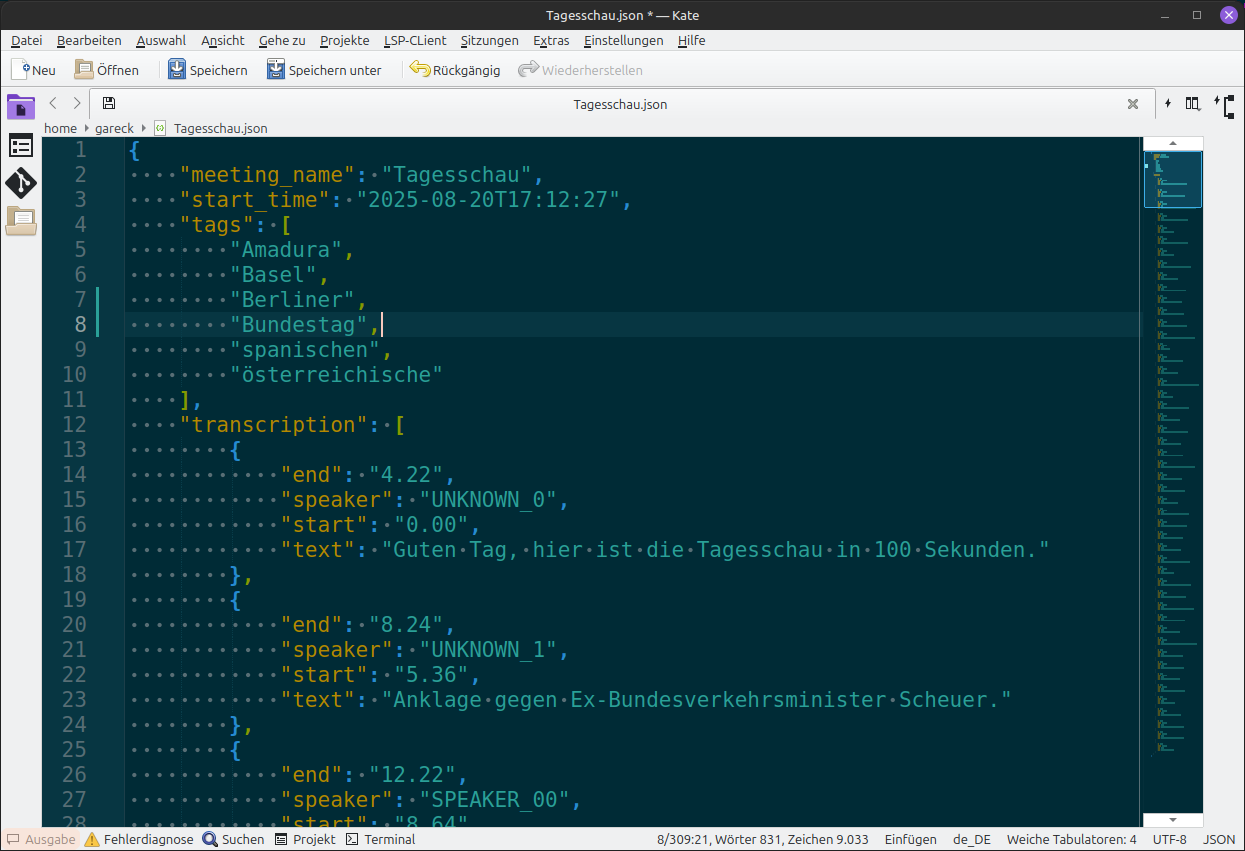
\includegraphics[width=0.7\linewidth]{Bilder/JSON}
    \caption[JSON]{Ausschnitt einer exportierten JSON-Datei in einem Texteditor}
    \label{pic:json}
\end{figure}


\begin{figure}
    \centering
    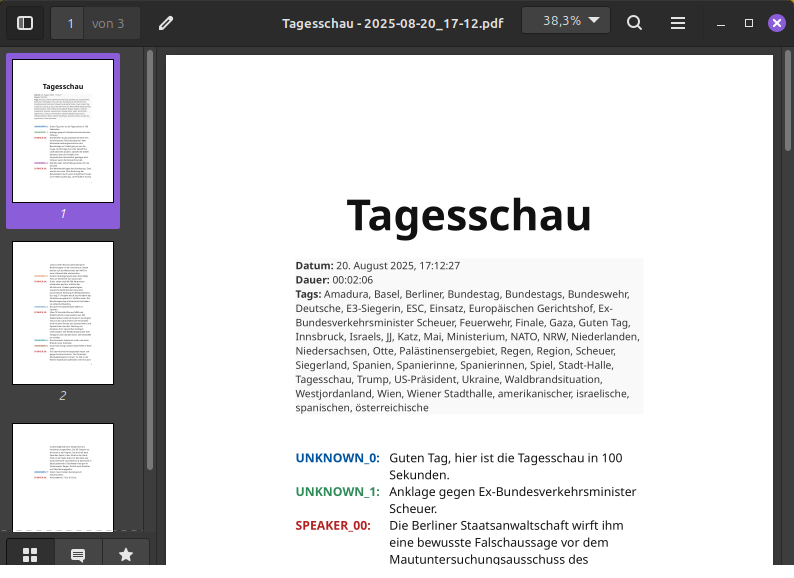
\includegraphics[width=0.7\linewidth]{Bilder/PDF}
    \caption[PDF]{Anfang eines Transkriptes im PDF-Format}
    \label{pic:pdf}
\end{figure}





\section{Anleitung und Benutzeroberfläche}
\label{sec:gui}
\authormargin{Mike Wild}

\subsection{Python-Installationsfenster}
\label{sub:install}

Wenn man das Programm das erste Mal startet, öffnet sich nicht das Hauptfenster der Anwendung, sondern es wird automatisch eine virtuelle Python-Umgebung eingerichtet, die alle benötigten Pakete und \ac{KI}-Modelle für die Transkription und andere Funktionen beinhaltet. Dies dient dazu, dass das Programm das System, auf dem es läuft, nicht verändert. Abbildung \ref{pic:Install} zeigt das Installationsfenster für die virtuelle Python-Umgebung. Die Installation übernimmt ein Shell- bzw. Batch-Skript. Die Ausgabe des Skripts wird im Fenster angezeigt. Das Skript kann später über den Menü-Punkt "Python neu-installieren" oder auch manuell erneut gestartet werden. Die nun installierte virtuelle Umgebung ist nicht zwangsläufig notwendig. Man kann die Installation abbrechen und das auf dem System installierte Python nutzen. Hierzu wird nach dem Abbrechen oder bei einem Installationsfehler zunächst das Einstellungsfenster (siehe Abb. \ref{pic:Settings} geöffnet.

\begin{figure}
    \centering
    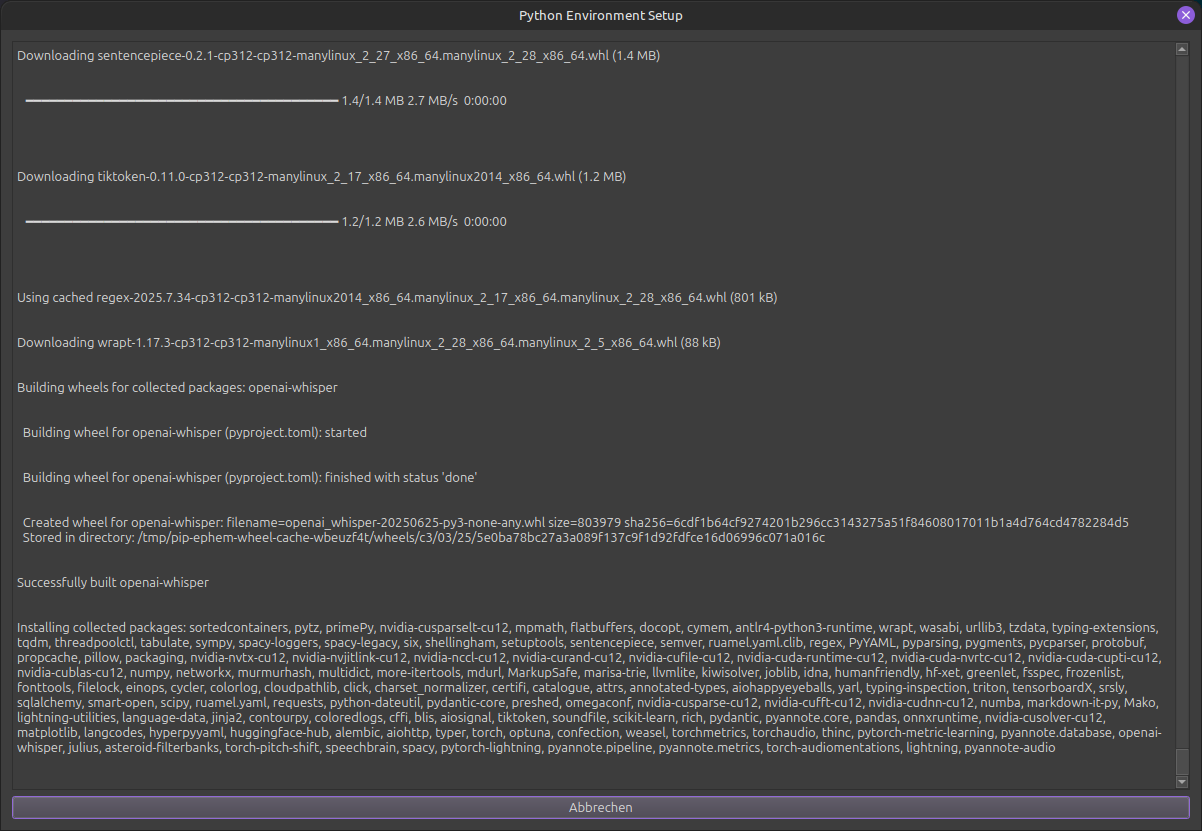
\includegraphics[width=0.7\linewidth]{Bilder/Python-Installationsfenster}
    \caption[Python-Installationsfenster]{Python-Installationsfenster}
    \label{pic:Install}
\end{figure}


\subsection{Einstellungsfenster}
\authormargin{Mike Wild}

\begin{figure}
    \centering
    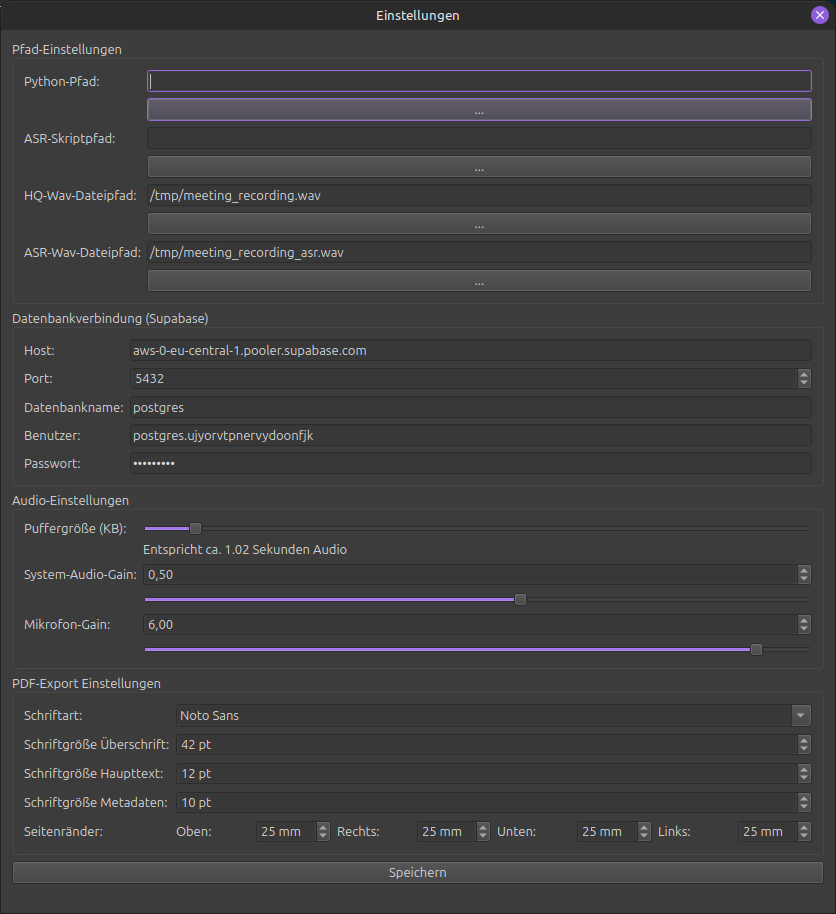
\includegraphics[width=0.7\linewidth]{Bilder/Einstellungen}
    \caption[Einstellungsfenster]{Einstellungsfenster}
    \label{pic:Settings}
\end{figure}


Dort muss unter dem Punkt \glqq Python-Pfad\grqq\ der Pfad zur ausführbaren Python-Datei (meist \glqq python3\grqq\ genannt) eingetragen werden. Hier kann die Datei aus einer beliebigen virtuellen Umgebung oder die Datei vom System eingetragen werden. Unter dem zweiten Punkt \glqq ASR-Skriptpfad\grqq\ muss ein Python-Skript zum Transkribieren eingetragen werden. Das Programm bietet momentan die beiden Möglichkeiten \glqq run\_asr.py\grqq\ und \glqq asr\_backend.py\grqq. Das erste Skript transkribiert das Audio erst hinterher, indem es eine Wav-Datei entgegennimmt. Es arbeitet mit pyannote und whisper. Das zweite Skript ist für die Echtzeitverarbeitung zuständig, näheres im Kapitel \ref{chap:ki} auf Seite \pageref{chap:ki}. Diese ersten zwei Punkte sind essentiell, damit das Programm wie vorgesehen arbeiten kann.

Mit den nächsten zwei Pfaden kann man angeben, wo das Programm die Audiodateien zwischenspeichert. Diese werden im Wav-Format gespeichert. Dabei steht \glqq HQ\grqq\ für \textbf{H}igh-\textbf{Q}uality, also die Audiodatei mit voller Qualität, und \glqq ASR\grqq\ für die downgesamplete Audiodatei zur nachträglichen Transkription. Standardmäßig werden für die diese beiden Dateien in einem Standardordner für temporäre Dateien gespeichert. Danach folgen Einstellungen zur Datenbankverbindung, wo die Transkripte gespeichert und abgerufen werden sollen. Hier ist eine \glqq Supabase\grqq\ Datenbank vorgesehen, kann aber ggf. durch eine andere Datenbank ausgetauscht werden, die im Qt-Framework vom Typ \glqq QPSQL\grqq\ ist und mit denselben Parametern sich verbinden lässt. Anschließend folgend die Audio-Einstellungen. Die Puffergröße bestimmt wie viel Audio-Daten zwischengespeichert werden, bevor sie auf die Festplatte in die Wav-Dateien geschrieben werden. Die beiden Gain-Werte ergeben das Mischungsverhältnis zwischen Mikrofon- und Systemaudio-Lautstärke. Diese sollten so eingestellt werden, dass in der resultierenden Audio-Datei die Lautstärke des Mikrofons genauso laut ist, wie die des Systemmix. Zuletzt folgen noch Einstellungen, um das Aussehen der PDF-Datei, die man aus dem Transkript erzeugen lassen kann, zu optimieren.


\subsection{Hauptfenster}
\authormargin{Mike Wild}
\label{sub:main}

\begin{figure}
    \centering
    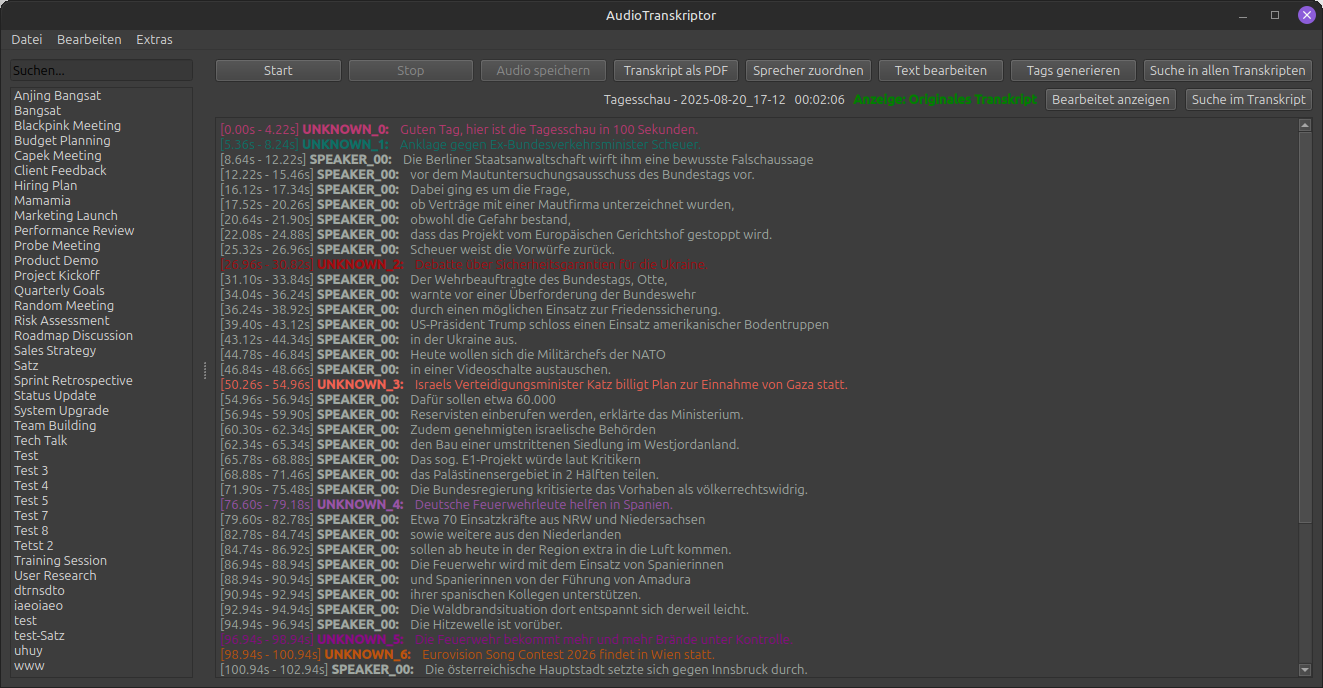
\includegraphics[width=0.7\linewidth]{Bilder/Applikation}
    \caption[Hauptfenster]{Hauptfenster der Applikation}
    \label{pic:App}
\end{figure}

Im Hauptfenster der Applikation befindet sich ganz oben die Menü-Leiste mit der man Transkripte speichern und laden kann, Änderungen rückgängig machen, Python neu installieren kann und das Einstellungsfenster öffnet. Bei MacOS befindet sich die Menüleiste nicht im Fenster, sondern am oberen Bildschirmrand. Auf der linken Seite sieht man die in der Datenbank gespeicherten Transkripte. Auf der rechten Seite sieht man zentral das gerade geladene Transkript und oberhalb davon die Bedienelemente. \glqq Start\grqq\  bzw. \glqq Stopp\grqq\  starten bzw. stoppen die Audioaufnahme. Erst nachdem eine Aufnahme beendet worden ist, kann man mit \glqq Audio speichern\grqq\ diese als Wav-Datei speichern. \glqq Transkript als PDF\grqq\  dient zum Exportieren des Transkriptes als PDF-Datei. \glqq Sprecher zuordnen\grqq\ (siehe Abschnitt \ref{sub:sprecher}) und \glqq Text bearbeiten\grqq\ (siehe Abschnitt \ref{sub:text}) dienen zum Manipulieren des Transkriptes. Mit \glqq Tags generieren\grqq\ werden über ein Python-Skript mittes spaCy Schlagworte zum gesamten Transkript erzeugt.

\authormargin{Yolanda Hadiana Fiska}
Der Button „Bearbeitet anzeigen“ ermöglicht es dem Benutzer, die Ansicht des geladenen Transkripts abhängig vom aktuellen Modus umzuschalten. Während die Option „Bearbeitet anzeigen“ zur redigierten Version des Transkripts wechselt, führt die Option „Original anzeigen“ zurück zur ursprünglichen Fassung. Der jeweils aktive Modus wird links neben diesem Umschaltknopf angezeigt. Darüber hinaus stehen dem Benutzer zwei Funktionen zur Protokollsuche zur Verfügung: Mit „Suche im Transkript“ kann innerhalb des aktuell geladenen Transkripts nach bestimmten Begriffen, Diskussionspunkten oder Informationen gesucht werden (siehe Abschnitt \ref{sub:lokalesuche}), während „Suche in allen Transkripten“ eine suchübergreifende Recherche über sämtliche vorhandenen Transkripte hinweg ermöglicht (siehe Abschnitt \ref{sub:globalesuche}).

\subsection{Sprecherbearbeitung}
\authormargin{Mike Wild}
\label{sub:sprecher}

\begin{figure}
    \centering
    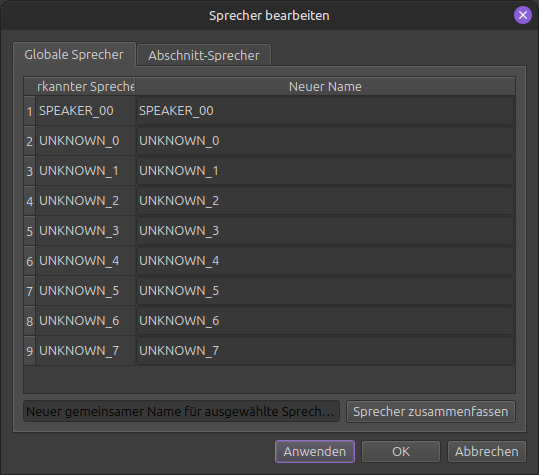
\includegraphics[width=0.7\linewidth]{Bilder/Sprecher1}
    \caption[Sprecherzuordnung]{Sprecherzuordnung für das gesamte Transkript}
    \label{pic:sprecher-allg}
\end{figure}

\begin{figure}
\centering
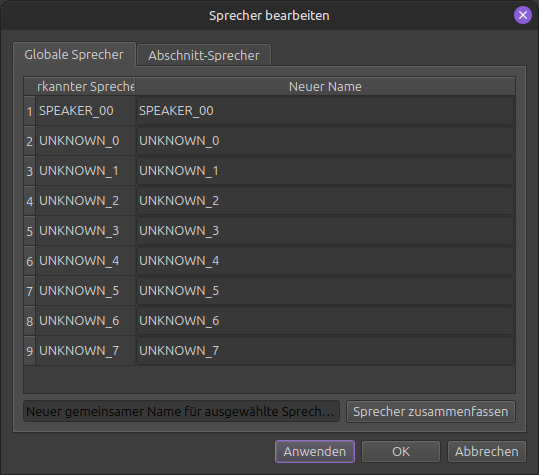
\includegraphics[width=0.7\linewidth]{Bilder/Sprecher1}
\caption[Sprecher ändern]{Sprecherzuordnung für einzelne Abschnitte}
\label{pic:sprecher-spez}
\end{figure}

Das Fenster zum Bearbeiten bzw. Zuordnen von Sprecher hat zwei Tabs, zwischen denen man wechseln kann. Der erste Tab (Abbildung \ref{pic:sprecher-allg}) dient dazu den Sprechern im Transkript, die automatisch mit \glqq SPEAKER\_XX\grqq\ (wobei XX eine zweistellige Nummer ist) benannt sind, echte Namen zuzuordnen. Das heißt, der Sprechername wird im gesamten Transkript ausgetauscht. Der zweite Tab (Abbildung \ref{pic:sprecher-spez}) ist dafür gedacht, falls die \ac{KI} den Text einen falschen Sprecher zuordnet, dies für diesen Textabschnitt zu korrigieren. Hier lassen sich die Spalten Start(-zeit) Ende (Endzeit) und Text nicht bearbeiten und dienen zum eindeutigen Erkennen des Abschnittes, von den man den Sprecher ändern möchte.


\subsection{Textbearbeitung}
\authormargin{Mike Wild}
\label{sub:text}

\begin{figure}
\centering
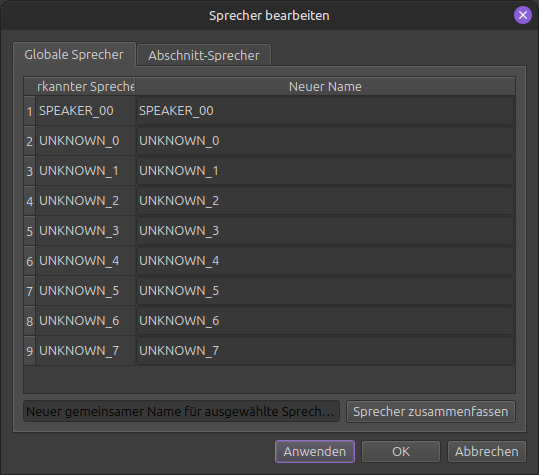
\includegraphics[width=0.7\linewidth]{Bilder/Sprecher1}
\caption[Textbearbeitung]{Textbearbeitung einzelner Abschnitte}
\label{pic:text}
\end{figure}

Mit dem Fenster in Abbildung \ref{pic:text} kann man den von der \ac{KI} automatisch transkribierten Text korrigieren, falls diese etwas fehlerhaft transkribiert hat. Die Spalten Start(-zeit) Ende (Endzeit) und Sprecher lassen sich hier nicht bearbeiten und dienen zum eindeutigen Erkennen des Abschnittes, den man bearbeiten möchte.

\subsection{Suche innerhalb eines Meetings}
\authormargin{Yolanda Hadiana Fiska}

\begin{figure}
\centering
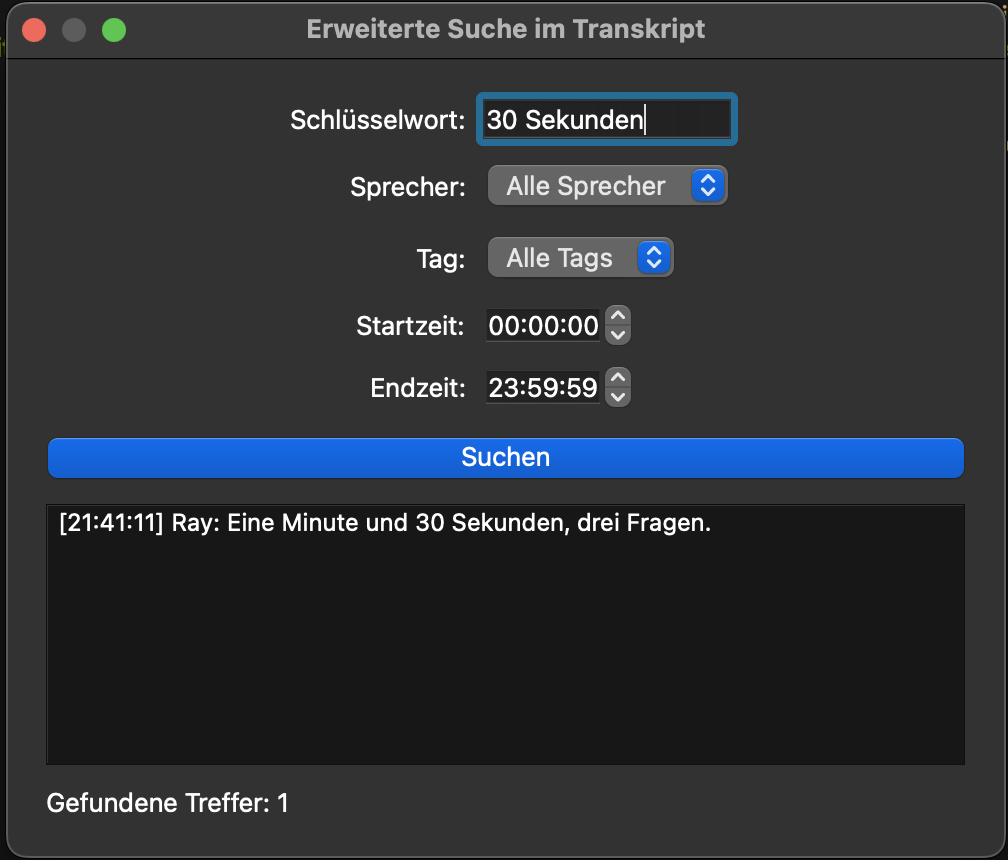
\includegraphics[width=0.7\linewidth]{Bilder/sucheInnerhalbMeeting.png}
\caption[Protokolsuche]{Systemansicht: Suche im Einzeltranskript}
\label{pic:lokalesuche}
\end{figure}

Das Fenster „Erweiterte Suche im Transkript“ (siehe Abbildung \ref{pic:lokalesuche} ) erlaubt eine gezielte Recherche innerhalb des aktuell geöffneten Transkripts. Es stellt verschiedene Such- und Filteroptionen zur Verfügung. Über das Feld „Schlüsselwort“ kann nach einem oder mehreren spezifischen Begriffen gesucht werden. Zusätzlich besteht die Möglichkeit, die Suche nach Sprecher (z. B. alle Sprecher oder ein bestimmter Redner) sowie nach Tags einzugrenzen. Ebenso können durch die Angabe einer Startzeit und Endzeit nur bestimmte Zeitbereiche des Transkripts berücksichtigt werden.

Die Ergebnisse der Suche werden in einer Liste dargestellt und enthalten die Zeitangabe, den Namen des Sprechers sowie die entsprechende Aussage. Wie in Abbildung \ref{pic:lokalesuche} dargestellt, werden die Eingabeoptionen für die Suche bereitgestellt.

\subsection{Globale Suche über alle Meetings}
\authormargin{Yolanda Hadiana Fiska}

Das Fenster „Erweiterte Mehrfachsuche“ (siehe Abbildung \ref{pic:globalesuche}) ermöglicht eine protokollübergreifende Recherche über sämtliche gespeicherten Transkripte. Im Unterschied zur Suche innerhalb eines einzelnen Protokolls werden hier alle verfügbaren Sitzungen in die Abfrage einbezogen. Die Filtermöglichkeiten entsprechen im Wesentlichen denen der Suche innerhalb eines Meetings, werden jedoch um zusätzliche Optionen wie die Eingrenzung nach Datum oder nach einem bestimmten Zeitraum erweitert.

\clearpage   % or \newpage
\begin{figure}[t]
\centering
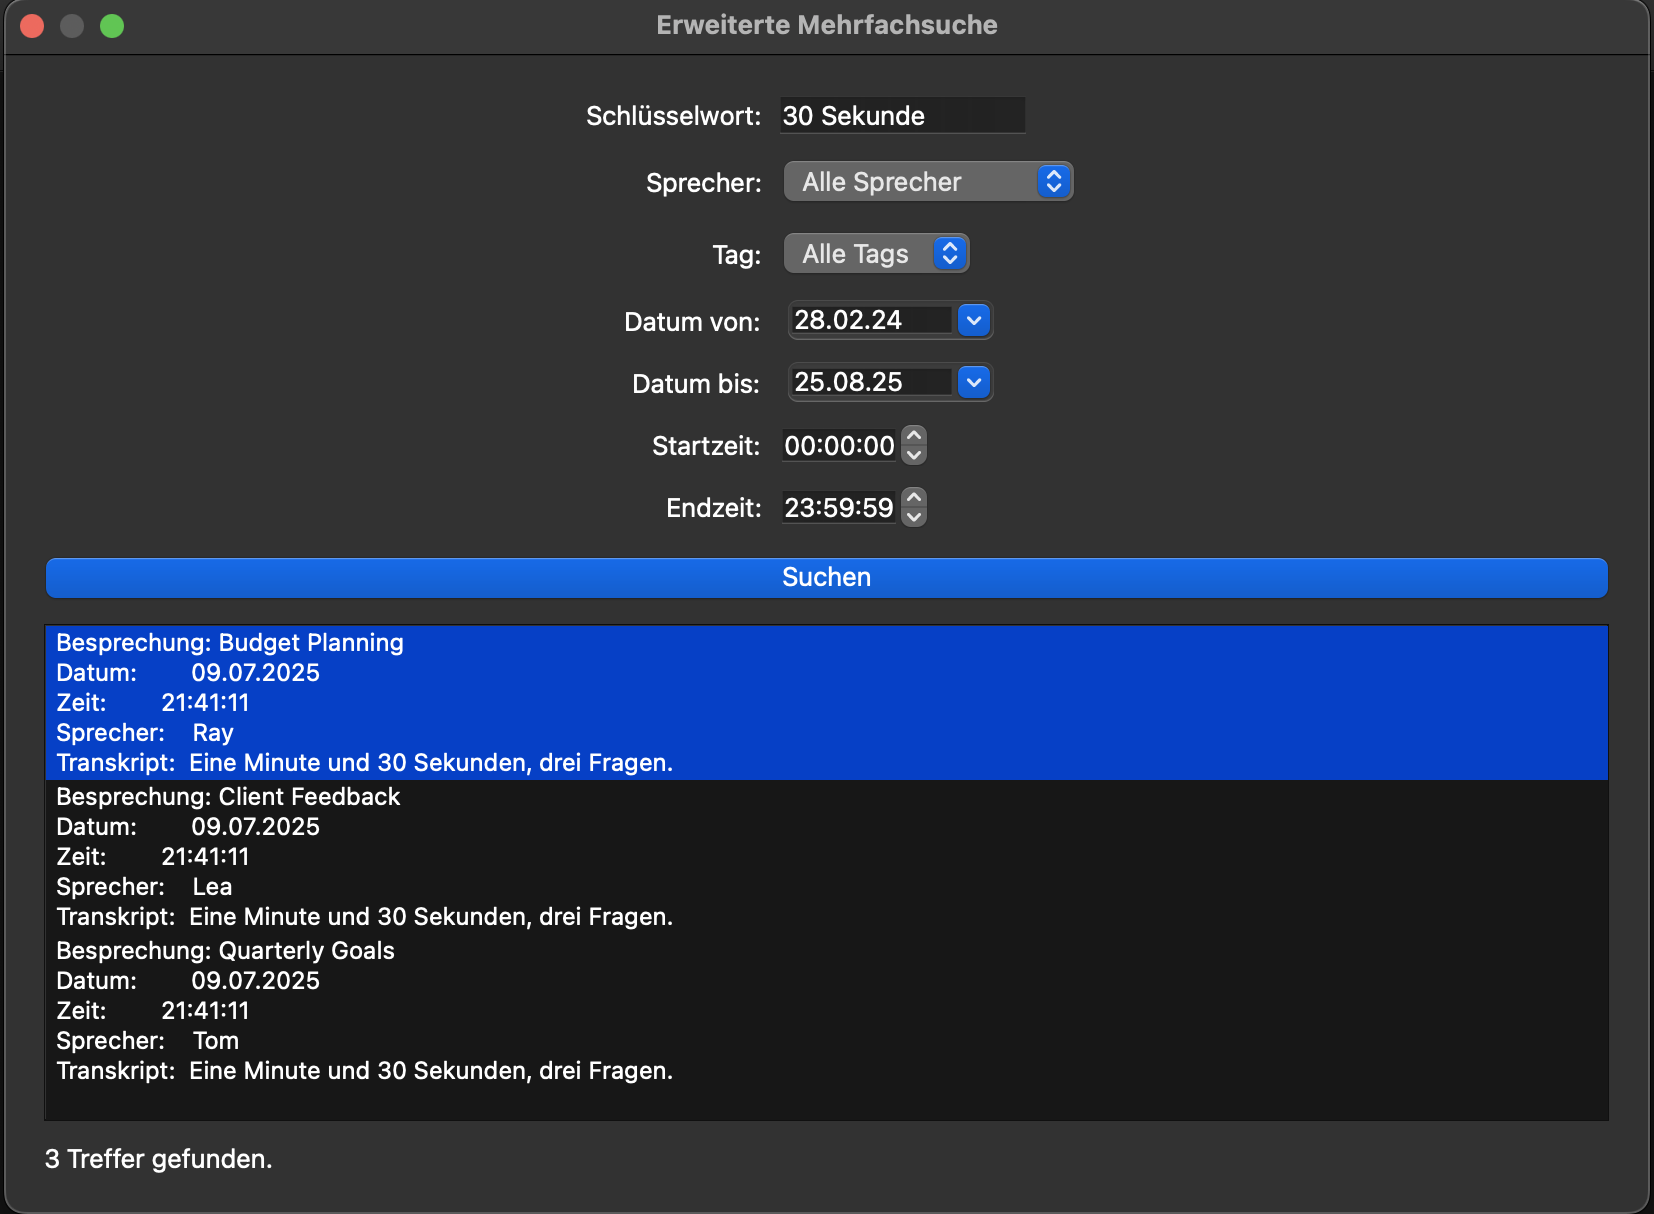
\includegraphics[width=0.7\linewidth]{Bilder/globaleSuche.png}
\caption[Protokolsuche]{Systemansicht: Suche über alle Transkripte}
\label{pic:globalesuche}
\end{figure}

Die Suchergebnisse werden in einer zentralen Liste angezeigt und enthalten neben dem Namen der Sitzung, dem Datum und dem Sprecher auch den Ausschnitt der Aussage, in dem das gesuchte Schlüsselwort vorkommt. Wie in Abbildung  \ref{pic:globalesuche}  dargestellt, kann durch Anklicken eines Eintrags direkt das entsprechende Meeting im Hauptfenster geladen werden. Dort werden die gesuchten Begriffe im Transkript hervorgehoben, sodass die relevanten Stellen unmittelbar erkennbar sind (Siehe Abbildung \ref{pic:markiertertreffer}). 

\begin{figure}[h]
\centering
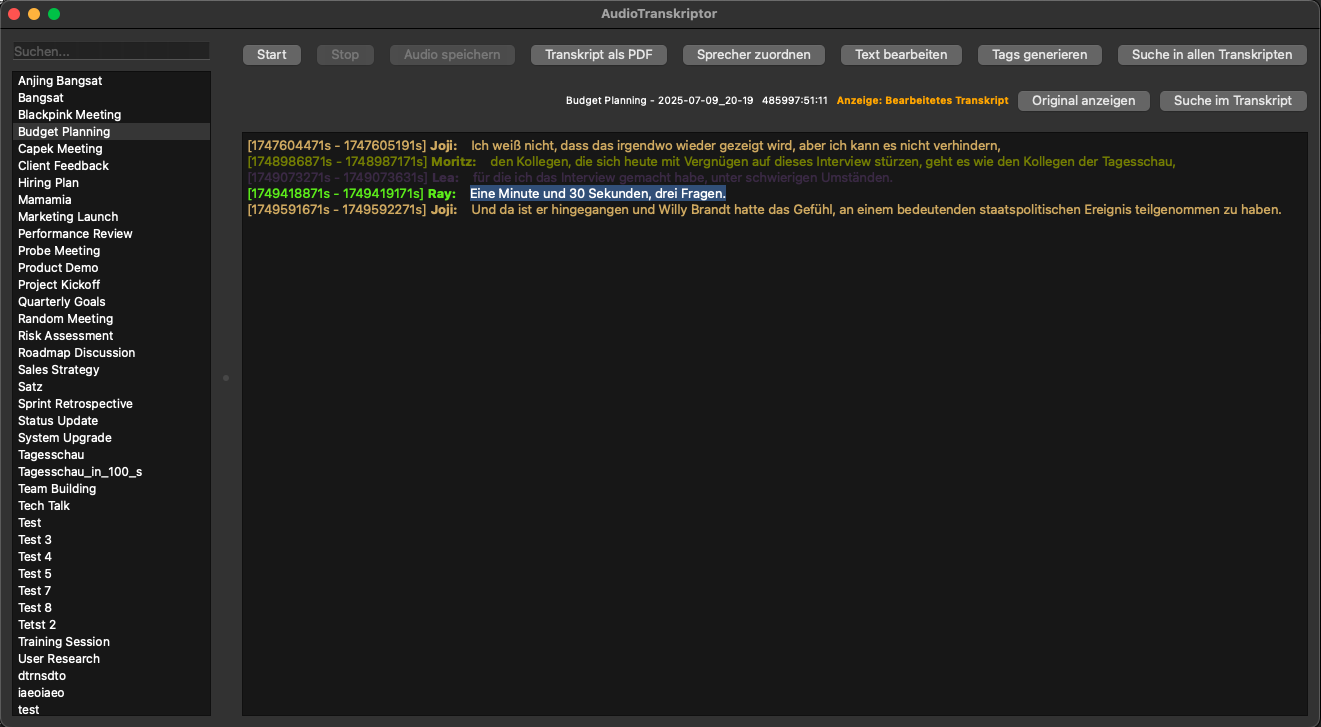
\includegraphics[width=0.7\linewidth]{Bilder/markierterTreffer}
\caption[Protokolsuche]{Darstellung eines Transkripts mit hervorgehobenen Suchergebnissen nach Auswahl eines Eintrags aus der Ergebnisliste}
\label{pic:markiertertreffer}
\end{figure}

\section{Workflow aus Anwendersicht}
\label{sec:workflow}
\authormargin{Mike Wild}

Angenommen man hat das Programm schon einmal gestartet, sodass die Python-Umgebung richtig aufgesetzt ist, dann sieht der typische Workflow mit dieser Applikation wie folgt aus. Das Programm startet mit dem Hauptfenster (vgl. Abschnitt \ref{sub:main}, Seite \pageref{sub:main}). Man drückt auf \glqq Start\grqq , hält sein Online-Meeting ab und drückt auf \glqq Stop\grqq . Danach kann man die Audiodatei speichern. Anschließend ordnet man den Sprecher die entsprechenden Namen zu, korrigiert ggf. den Text, generiert Schlagworte für das Transkript und speichert es in der Datenbank. Bei Bedarf exportiert man das Transkript als PDF-Datei. Danach ist man bereit für das nächste Meeting.


%----------- File: Kapitel/konzeption_architektur.tex -----------

\chapter{Konzeption \& Architektur der Anwendung}
\label{chap:architektur}
\authormargin{Mike Wild}

Dieses Kapitel beschreibt die fachliche Konzeption und die Softwarearchitektur der Anwendung. Ziel ist eine plattformübergreifende, echtzeitfähige Erfassung von System- und Mikrofon-Audio, deren automatische Transkription und Weiterverarbeitung und Verwaltung des Textes.Der Fokus dieses Kapitels liegt auf den architektonischen Entscheidungen, die getroffen wurden, um die zentralen Herausforderungen zu bewältigen. Es werden die Schlüsselkomponenten vorgestellt und die zugrundeliegenden Design Patterns erläutert.


\section{Architektonischer Überblick und Design-Prinzipien}
\authormargin{Mike Wild}

Die Software-Architektur der Applikation basiert auf den \textbf{\ac{SOLID}}-Prinzipien der objektorientierten Programmierung.

\grqq Das \textbf{Single-Responsibility-Prinzip} besagt, dass jede Klasse nur eine einzige Verantwortung haben solle. Verantwortung wird hierbei als „Grund zur Änderung“ definiert. […] Das \textbf{Open-Closed-Prinzip} besagt, dass Software-Einheiten (hier Module, Klassen, Methoden usw.) Erweiterungen möglich machen sollen (dafür offen sein), aber ohne dabei ihr Verhalten zu ändern (ihr Sourcecode und ihre Schnittstelle sollte sich nicht ändern). […] Das \textbf{\ac{LSP}} oder Ersetzbarkeitsprinzip fordert, dass eine Instanz einer abgeleiteten Klasse sich so verhalten muss, dass jemand, der meint, ein Objekt der Basisklasse vor sich zu haben, nicht durch unerwartetes Verhalten überrascht wird, wenn es sich dabei tatsächlich um ein Objekt eines Subtyps handelt. […] Das \textbf{Interface-Segregation-Prinzip} dient dazu, zu große Interfaces aufzuteilen. Die Aufteilung soll gemäß den Anforderungen der Clients an die Interfaces gemacht werden – und zwar derart, dass die neuen Interfaces genau auf die Anforderungen der einzelnen Clients passen. Die Clients müssen also nur mit Interfaces agieren, die das und nur das können, was die Clients benötigen. […] Das \textbf{Dependency-Inversion-Prinzip} beschäftigt sich mit der Reduktion der Kopplung von Modulen. Es besagt, dass Abhängigkeiten immer von konkreteren Modulen niedriger Ebenen zu abstrakten Modulen höherer Ebenen gerichtet sein sollten.  \grqq\ \cite{wiki:solid}


Von der Architektur her wird auf die Trennung von Verantwortlichkeiten geachtet. So ist die Benutzeroberfläche (\texttt{MainWindow}) von der Backend-Logik entkoppelt. Aufwendige Operationen, wie die Audio-Aufnhame, das Schreiben von Dateien und die Kommunikation mit externen Python-Prozessen werden in separate Hintergrund-Threads und spezialisierte Manager-Klassen ausgelagert. Dieser Ansatz stellt sicher, dass die \ac{GUI} jederzeit reaktionsfähig bleibt.



\section{Hauptkomponenten}
\authormargin{Mike Wild}

Hier wird ein kurzer Überblick über die wichtigsten Komponenten der Anwendung gezeigt. Diese sind:

\begin{itemize}
    \item \textbf{\texttt{MainWindow}}: Agiert als zentrale \textbf{Controller}-Instanz. Sie initialisiert alle Sub-Systeme, stellt die GUI dar und reagiert auf Benutzerinteraktionen, indem sie Aufgaben an die zuständigen Manager-Klassen delegiert.
    \item \textbf{Manager-Klassen (\texttt{FileManager}, \texttt{AsrProcessManager}, etc.)}: Kapseln spezifische Logikbereiche. Sie steuern externe Prozesse und abstrahieren den Dateizugriff.
    \item \textbf{\texttt{Transcription}}: Dient als zentrales \textbf{Datenmodell (Model)}, das alle Informationen zu einem Meeting enthält und als alleinige Quelle der Wahrheit (\glqq Single Source of Truth\grqq) fungiert.
    \item \textbf{\texttt{AudioFactory}}: Erzeugt plattformabhängig das richtige Audio-Aufnahme-Objekt und gibt es als \texttt{CaptureThread} zurück.
    \item \textbf{\texttt{CaptureThread}}: Ist eine abstrakte Basisklasse, die die plattformabhängigen Audio-Aufnahmen kapselt und gleichzeitig mittels \texttt{QWaitCondition} dafür sorgt, dass Ressourcen gespart werden, indem der Thread nur dann arbeitet, wenn auch Daten vorhanden sind und ansonsten schläft.
    \item \textbf{Audio-Threads (\texttt{CaptureThread}, \texttt{WavWriterThread})}: Implementieren das \textbf{Producer-Consumer-Pattern}. Der \texttt{CaptureThread} produziert Audiodaten, während der \texttt{WavWriterThread} diese konsumiert und auf die Festplatte schreibt.
\end{itemize}


\section{Threading- und Synchronisationskonzept}
\label{sec:threading}
\authormargin{Mike Wild}

Die Audioaufnahme und das Dateischreiben laufen in eigenen Threads. Der GUI-Thread bearbeitet ausschließlich Benutzerinteraktionen und reagiert über Signale/Slots:

\begin{itemize}
    \item \textbf{CaptureThread} (Audio): nicht-blockierendes Einlesen; Datenübergabe via \texttt{emit pcmChunkReady(...)} an den \texttt{WavWriterThread} mit \texttt{Qt::QueuedConnection}.
    \item \textbf{WavWriterThread}: wartet auf Daten, schreibt blockweise, finalisiert Header.
    \item \textbf{GUI-Thread}: steuert mit Start/Stop; aktualisiert Anzeigen (Zeitlabel / Status); lässt bei \texttt{Audio speichern} die HQ-Wav-Datei via \texttt{QtConcurrent::run} kopieren; verwaltet externe Prozesse via \texttt{QProcess}.
\end{itemize}

Das Beenden wird explizit orchestriert: \texttt{stopCapture()} beendet den inneren Loop, das \texttt{stopped}-Signal initiiert \texttt{stopWriting()}, anschließend löst \texttt{finishedWriting} den \ac{ASR}-Anstoß aus. \texttt{shutdown()}-Methoden stellen einen sauberen Thread-Stopp mit \texttt{wait()} sicher.


\section{Fehlerbehandlung und Cleanup}
\label{sec:cleanup}
\authormargin{Mike Wild}

Fehler im Initialisieren von Audio-Backends führen zu einem definierten Abbruch mit Aufräumen (\texttt{PulseAudio}-Module entladen; \texttt{WASAPI}-Interfaces \emph{safe release}). Beim Beenden der Anwendung werden Aufnahme- und Writer-Thread via \texttt{shutdown()} synchron gestoppt. Der \texttt{AsrProcessManager} signalisiert Erfolgs-/Fehlerzustände an die \ac{GUI}; Fehlermeldungen aus \emph{stderr} werden an die Nutzer weitergereicht.

\section{Konfigurierbarkeit}
\label{sec:config}
\authormargin{Mike Wild}

Zentrale Parameter werden über \texttt{QSettings} verwaltet: Lautstärkegewichte (\texttt{sysGain}, \texttt{micGain}), Puffergröße, Größe und Position des Fensters, Pfade der Python-Umgebung und \ac{ASR}-Skripte. Damit sind Build- und Laufzeitbelange getrennt und reproduzierbar dokumentiert.



\section{Zusammenfassung}
\authormargin{Mike Wild}
Die Architektur separiert Aufgaben konsequent: Audioaufnahme (plattformnah) in
spezialisierten Threads, persistentes Schreiben als eigenständige Stufe, \ac{ASR} als externer Prozess sowie eine \ac{GUI}, die lediglich orchestriert. Die lose Kopplung über Signale/Slots und Prozesse schafft Robustheit, Testbarkeit und Erweiterbarkeit.

%----------- File: Kapitel/implementierung.tex -----------

\chapter{Implementierung der Schlüsselkomponenten}
\label{chap:implementierung}
\authormargin{Mike Wild}

Aufbauend auf dem in Kapitel \ref{chap:architektur} vorgestellten Konzept, erläutert dieses Kapitel die konkrete technische Umsetzung der zentralen Komponenten der Applikation. Der Schwerpunkt liegt auf der Realisierung der plattformübergreifenden Audio-Aufnahme, der Synchronisation, der Audio-Streams und der Anbindung der externen KI-Module.


\section{Die plattformübergreifende Audio-Aufnahme}
\label{sec:audio_aufnahme}
\authormargin{Mike Wild}

Die größte Herausforderung bei der Audio-Aufnahme war die Inkompatibilität der nativen Audio-Schnittstellen der Zielplattformen MacOS, Windows (WASAPI) und Linux (PulseAudio). Um eine wartbare und erweiterbare Lösung zu schaffen, wurde eine Abstraktionsschicht implementiert, die auf zwei etablierten Software-Entwurfsmustern basiert.

\subsection{Abstraktion durch Design Patterns}
\authormargin{Mike Wild}

Die Entkopplung der plattformspezifischen Logik von der Hauptanwendung wurde durch die kombinierte Anwendung des \textit{Abstract Factory}- und des \textit{Template Method}-Patterns erreicht.

\begin{itemize}
    \item \textbf{Template Method Pattern:} Die abstrakte Basisklasse \texttt{CaptureThread} definiert das Grundgerüst des Aufnahme-Algorithmus in ihrer \texttt{run()}-Methode. Dieser Ablauf -- Initialisieren, Aufnahmeschleife, Aufräumen -- ist für alle Plattformen identisch. Die konkreten, plattformabhängigen Implementierungsschritte werden als rein virtuelle Methoden (\texttt{initializeCapture()}, \texttt{captureLoopIteration()}, \texttt{cleanupCapture()}) deklariert, die von den abgeleiteten Klassen überschrieben werden müssen.
    \item \textbf{Abstract Factory Pattern:} Die \texttt{AudioFactory} dient als zentrale Erzeugungsinstanz. Ihre statische Methode \texttt{createThread()} wählt zur Kompilierzeit mittels Präprozessor-Direktiven (\texttt{\#if defined(Q\_OS\_WIN)}) die korrekte, konkrete \texttt{CaptureThread}-Implementierung aus und instanziiert diese. Dadurch bleibt der restliche Code, insbesondere die \texttt{MainWindow}, vollständig agnostisch gegenüber dem zugrundeliegenden Betriebssystem.
\end{itemize}

Wie die Aufnahme der Audiosignale konkret implementiert ist, kann man in den nachfolgenden Kapiteln sehen. Die Audioaufnahme unter Windows in Kapitel \ref{chap:audio_windows} ab Seite \pageref{chap:audio_windows}, für Linux (nur PulseAudio) in Kapitel \ref{chap:audio_linux} ab Seite \pageref{chap:audio_linux} und für MacOS in Kapitel \ref{chap:audio_mac} ab Seite \pageref{chap:audio_mac}.



\section{Anbindung der KI-Module}
\label{sec:ki_anbindung}
\authormargin{Mike Wild}

Die Ausführung der rechenintensiven Python-Skripte für die Transkription und Tag-Erstellung ist in den Manager-Klassen \texttt{AsrProcessManager} und \texttt{TagGeneratorManager} gekapselt. Beide folgen demselben Entwurfsmuster, um die asynchrone und sichere Kommunikation zwischen C++ und Python zu gewährleisten.

Der Manager startet das jeweilige Python-Skript als externen Prozess mittels \texttt{QProcess}. Die Datenübergabe von C++ nach Python erfolgt über die Standard-Eingabe (stdin) des Prozesses. Dies ist besonders für die Tag-Generierung vorteilhaft, da so beliebig lange Texte ohne Beschränkungen durch Kommandozeilenargumente übergeben werden können. Nach dem Schreiben der Daten wird der Schreibkanal mit \texttt{closeWriteChannel()} geschlossen, was dem Python-Skript das Dateiende (EOF) signalisiert und dessen Verarbeitung anstößt.

Die Ergebnisse werden vom Python-Skript zeilenweise auf die Standard-Ausgabe (stdout) geschrieben. Der C++-Manager liest diese Ausgabe, parst sie und kommuniziert die fertigen Ergebnisse (z.B. ein \texttt{MetaText}-Segment oder eine Liste von Tags) über Qt-Signale an die \texttt{MainWindow}. Dieser ereignisbasierte Ansatz stellt sicher, dass die GUI auch während der Analyse durch die Python-Skripte nicht blockiert wird.


\section{Nachgelagerte Transkription}
\label{sec:whisper}
\authormargin{Mike Wild}

Die Aufgabenstellung hat eine Transkription in Echtzeit gefordert, dennoch ist in der Applikation auch noch eine nachgelagerte Transkription mit eingebaut. Dies hat zweierlei Gründe. Zum einen würde Übergangsweise eine Lösung benötigt bis das eigentliche KI-Modell fertig war, um die Applikation vollständig zu Testen und die anderen Features entwickeln zu können. Und zum anderen ist das eine gute Möglichkeit die Ergebnisse der Echtzeittranskription zu vergleichen und zu evaluieren. Das hier eingesetzte Python-Skript (\texttt{run\_asr.py}) verwendet \texttt{pyannote} für die Sprecherdiarisierung und \texttt{whisper} für die Transkription. Dies lässt sich aber leicht ändern, sodass beispielsweise die Transkription über \texttt{google} erfolgen kann. Da die nachgelagerte Transkription nicht Teil der Aufgabenstellung ist, wird hier auch nicht näher darauf eingegangen. Somit beschäftigt sich Kapitel \ref{chap:ki} mit der echtzeitfähigen Transkription.

\section*{Hinweis}
Aufgrund des Zeitmangels sind die Komponenten: \glqq Audioaufnahme unter MacOS\grqq\ und \glqq Echtzeittranskription\grqq\ noch nicht vollständig in der endgültigen Version der Applikation (main-Branch) enthalten. Diese sind jedoch einzeln in einer eigenen Version integriert (siehe Paki-Branch, bzw. Fabian-Branch).

%----------- File: Kapitel/audio_windows.tex -----------

\chapter{Audioaufnahme unter Windows (WASAPI)}
\label{chap:audio_windows}
\authormargin{Mike Wild}


Unter Windows wird die Audioaufnahme über die Windows Audio Session API (WASAPI) realisiert. Die Klasse \texttt{WinCaptureThread} kombiniert \emph{Loopback}-Capture für den Systemmix (Wiedergabe) und reguläres Capture für das Mikrofon (Aufnahme). Die Implementierung adressiert zwei zentrale Herausforderungen:
(I) Synchronisation zweier unabhängiger Geräte mit potentiell unterschiedlicher Samplerate und
(II) robuste Pufferung/Entkopplung durch ringförmige FIFOs und einen zeitbasierten Resampling-Ansatz.


\section{Designziele und Grundidee}
\label{sec:wasapi_ziele}
\authormargin{Mike Wild}

\begin{itemize}
    \item \textbf{Gleichzeitiges Erfassen} von System- und Mikrofon-Stream via getrennte  \texttt{IAudioClient}/\texttt{IAudioCaptureClient}-Paare.
    \item \textbf{Zeitbasierte Synchronisation}: statt paketgetriebener Taktung wird die exakte vergangene Zeit per \texttt{QueryPerformanceCounter} ermittelt; daraus wird die zu generierende Zielframezahl bei 48\,kHz abgeleitet.
    \item \textbf{Sanftes Resampling}: FIFO-Puffer + kontinuierliche Lese-Positionen     (\texttt{m\_resampPosSys/Mic}) erlauben interpolationsfreies (nearest/linear) Sampling; hier: Sample-At-Position via Ringpuffer.
    \item \textbf{Thread-Lebenszyklus} durch Basisklasse \texttt{CaptureThread} (Warten $\rightarrow$ Initialisieren $\rightarrow$ Loop $\rightarrow$ Cleanup).
\end{itemize}


\section{Initialisierung (\texttt{initializeCapture()})}
\label{sec:wasapi_init}
\authormargin{Mike Wild}

\subsection*{Ablaufbeschreibung}
\begin{enumerate}
    \item \textbf{Geräte-Enumerator}: \texttt{MMDeviceEnumerator} erzeugen.
    \item \textbf{Default-Geräte}: Wiedergabe (\texttt{eRender}, \texttt{eConsole})
    für Loopback, Aufnahme (\texttt{eCapture}, \texttt{eConsole}) für Mikrofon.
    \item \textbf{IAudioClient}: je Gerät aktivieren und \texttt{GetMixFormat()} abfragen
    (native Samplerate/Kanalzahl).
    \item \textbf{Initialize()}: Systemclient im Shared-Mode mit
    \texttt{AUDCLNT\_STREAMFLAGS\_LOOPBACK}; Mikrofonclient im Shared-Mode.
    \item \textbf{IAudioCaptureClient}: je Client abrufen; Puffergrößen vorbereiten.
    \item \textbf{Start()}: beide Streams starten.
\end{enumerate}



\subsection*{Auszug (Listing)}
\begin{lstlisting}[language=C++,caption={WASAPI-Setup (vereinfacht)},label={lst:wasapi_init}]
    hr = CoCreateInstance(__uuidof(MMDeviceEnumerator), nullptr, CLSCTX_ALL,
    IID_PPV_ARGS(&m_deviceEnumerator));
    m_deviceEnumerator->GetDefaultAudioEndpoint(eRender, eConsole, &m_deviceSys);
    m_deviceSys->Activate(__uuidof(IAudioClient), CLSCTX_ALL, nullptr,
    reinterpret_cast<void**>(&m_audioClientSys));
    WAVEFORMATEX* wfexSys = nullptr;
    m_audioClientSys->GetMixFormat(&wfexSys);
    m_audioClientSys->Initialize(AUDCLNT_SHAREMODE_SHARED,
    AUDCLNT_STREAMFLAGS_LOOPBACK,
    10000000, 0, wfexSys, nullptr);
    CoTaskMemFree(wfexSys);
    m_audioClientSys->GetService(IID_PPV_ARGS(&m_captureClientSys));
    // ... analog fuer Mic (ohne LOOPBACK-Flag)
\end{lstlisting}


\section{Zeitbasierte Synchronisation \& Resampling (\texttt{captureLoopIteration()})}
\label{sec:wasapi_loop}
\authormargin{Mike Wild}

Die Besonderheit bei der Audioaufnahme unter Windows mittels \ac{WASAPI} ist, dass man diese nicht paketgetrieben \emph{zu takten} kann. Denn dann würden nur dann Daten aufgezeichnet werden, wenn auch tatsächlich Audiodaten zur Verfügung stehen, d.h. es wird keine Stille aufgezeichnet. Dies führt neben der falschen Aufnahme-Dauer auch noch zu dem Problem, dass die Audiosignale vom System und vom Mikrofon nicht mehr synchron währen. Deswegen muss, mithilfe eines sehr genauen Timers, die vergangene Zeit seit dem letzten Verarbeiten von Audiosignalen gemessen werden, und die Audiodaten um die Stille ergänzt werden. Somit wird die in der aktuellen Iteration vergangene Zeit $\Delta t$ per \texttt{QueryPerformanceCounter} bestimmt. Daraus ergeben sich die zu erzeugenden Ziel-Frames bei 48\,kHz:
\[
N_\text{target} := \lfloor 48000 \cdot \Delta t + \text{Akkumulator} \rfloor.
\]
Für jedes Zielsample werden die momentanen Werte aus den FIFO-Puffern mit
Positionszeigern \texttt{m\_resampPosSys/Mic} gelesen. Dieses Schema erzeugt
bei ausbleibenden Paketen faktisch Stille, hält aber die Streams zueinander synchron.



%----------- File: Kapitel/audio_linux.tex -----------

\chapter{Audioaufnahme unter Linux (PulseAudio)}
\label{chap:audio_linux}
\authormargin{Mike Wild}

Dieses Kapitel beschreibt die plattformspezifische Audioaufnahme unter Linux mittels \emph{PulseAudio}. Andere Audio-Systeme werden derzeit nicht unterstützt. Die Klasse \texttt{PulseCaptureThread} leitet von der abstrakten Basisklasse \texttt{CaptureThread} ab und implementiert die Initialisierung, den Aufnahme-Loop sowie das Aufräumen der PulseAudio-Ressourcen. Kernidee ist die gleichzeitige Erfassung des \emph{Systemmixes} (Wiedergabegerät) und des \emph{Mikrofons}, deren Signale in 32-bit-Float gemischt, gegen Clipping begrenzt und anschließend an den \texttt{WavWriterThread} übertragen werden.


\section{Ziele und Designentscheidungen}
\label{sec:linux_ziele}
\authormargin{Mike Wild}

Die Linux-Implementierung verfolgt folgende Ziele:
\begin{itemize}
    \item \textbf{Gleichzeitige Erfassung} von System-Audio (\enquote{what-you-hear}) und Mikrofon.
    \item \textbf{Robustheit} durch explizites Fehler-Handling beim Laden desModuls und beim Öffnen der PulseAudio-Streams.
    \item \textbf{Einfache Parametrisierung} (z.\,B.\ Lautstärkeverhältnisse) via \texttt{QSettings}.
    \item \textbf{Streckenweise Entkopplung} durch den \texttt{CaptureThread}-Lebenszyklus (Warteschleife $\rightarrow$ Initialisierung $\rightarrow$ Aufnahme $\rightarrow$ Cleanup).
\end{itemize}


\section{Architektur und Datenpfad}
\label{sec:linux_architektur}
\authormargin{Mike Wild}

Die Initialisierung richtet zwei Aufnahmequellen ein:
\begin{enumerate}
    \item \textbf{Systemmix} via \texttt{\$DefaultSink.monitor}.
    \item \textbf{Mikrofon} via \emph{virtuelle Senke}: \texttt{module-null-sink} (\enquote{MicSink}) und ein \texttt{module-loopback} vom Standard-\emph{Source} auf diese Senke; abgehört wird \texttt{mic\_sink.monitor}.
\end{enumerate}

Beide Quellen werden mit \texttt{pa\_simple\_new} als Float32LE, $48$\,kHz, Stereo geöffnet. Im Aufnahmeloop werden Blockweise $N=1024$ Frames pro Quelle gelesen, in einem Mischpuffer skaliert (\texttt{sysGain}, \texttt{micGain}) und mit \texttt{qBound} gegen Clipping begrenzt. Der gemischte Block wird als \texttt{QList<float>} per \texttt{emit pcmChunkReady(chunk)} an den \texttt{WavWriterThread} übergeben (vgl.\ Kapitel \ref{chap:wav_thread}). Anders als bei der Audioaufnahme unter Windows (siehe Abschnitt \ref{sec:wasapi_loop}), kann hier auf ein Timer verzichtet werden, da \texttt{PulseAudio} auch bei Stille Audiodaten liefert.

\section{Initialisierungsschritte (\texttt{initializeCapture()})}
\label{sec:linux_initialize}
\authormargin{Mike Wild}

\subsection*{Ablauf in Worten}
\begin{enumerate}
    \item \textbf{Einstellungen laden}: \texttt{sysGain}, \texttt{micGain} aus \texttt{QSettings}.
    \item \textbf{Standardgeräte ermitteln}: \texttt{pactl info} parsen (Sprache robust: EN/DE).
    \item \textbf{Virtuelle Module laden}: \texttt{module-null-sink} $\rightarrow$ \texttt{mic\_sink},
    \texttt{module-loopback} (Mikrofon $\rightarrow$ \texttt{mic\_sink}).
    \item \textbf{PulseAudio-Streams öffnen}:
    \texttt{pa\_simple\_new} für \texttt{\$DefaultSink.monitor} (Systemmix) und \texttt{mic\_sink.monitor}.
    \item \textbf{Puffer vorbereiten}: \texttt{bufSys}, \texttt{bufMic}, \texttt{bufMix} mit $N\times 2$ (Stereo).
\end{enumerate}



\subsection*{Auszug (Listing)}
\begin{lstlisting}[language=C++,caption={Ermitteln der Default-Geräte und Laden der PulseAudio-Module},label={lst:pulse-modules}]
    QProcess infoProc;
    infoProc.start("pactl", {"info"});
    infoProc.waitForFinished(500);
    QString info = QString::fromUtf8(infoProc.readAllStandardOutput());

    QRegularExpression reEnSink(R"(Default Sink:\s*(\S+))"),
    reDeSink(R"(Standard-Ziel:\s*(\S+))"),
    reEnSrc (R"(Default Source:\s*(\S+))"),
    reDeSrc (R"(Standard-Quelle:\s*(\S+))");

    QString origSink = ...; // via RegEx
    QString origSource = ...;

    auto loadModule = [&](const QString& params)->int {
        QProcess p; p.start("pactl", QStringList{"load-module"} << params.split(' '));
        p.waitForFinished();
        bool ok; int id = QString::fromUtf8(p.readAllStandardOutput()).trimmed().toInt(&ok);
        return ok ? id : -1;
    };

    m_modNull = loadModule("module-null-sink sink_name=mic_sink sink_properties=device.description=MicSink");
    m_modLoop = loadModule(QString("module-loopback source=%1 sink=mic_sink").arg(origSource));
\end{lstlisting}

\section{Aufnahme-Loop (\texttt{captureLoopIteration()})}
\label{sec:linux_loop}
\authormargin{Mike Wild}

\subsection*{Ablauf in Worten}

In jeder Iteration werden $N=1024$ Frames pro Quelle synchron gelesen. Schlägt \texttt{pa\_simple\_read} fehl, wird die Session beendet (\texttt{stopCapture()}). War das Lesen erfolgreich, werden anschließend System- und Mikrofonsamples gewichtet addiert:

\begin{equation*}
    \mathrm{mix}[i] = \mathrm{qBound}\bigl(-1,\; \mathrm{sysGain}\cdot \mathrm{sys}[i] + \mathrm{micGain}\cdot \mathrm{mic}[i],\; 1\bigr).
\end{equation*}

Der resultierende Stereo-Block \texttt{bufMix} wird in eine \texttt{QList<float>} kopiert, als \texttt{chunk} emittiert und vom \texttt{WavWriterThread} asynchron weiterverarbeitet bzw. resamplet und ans Echtzeit-Transkriptions-Skript weitergereicht.


\section{Aufräumen (\texttt{cleanupCapture()})}
\label{sec:linux_cleanup}
\authormargin{Mike Wild}

Beim Beenden werden offene Restpuffer optional geleert (\enquote{drain}) und beide \texttt{pa\_simple}-Streams freigegeben. Anschließend entlädt die Implementierung die geladenen PulseAudio-Module (\texttt{module-loopback}, \texttt{module-null-sink}), um das System in den Ausgangszustand zurückzuversetzen. Dies ist insbesondere in Multi-App-Szenarien wichtig, um Seiteneffekte zu vermeiden.


\section{Parametrisierung und Grenzfälle}
\label{sec:linux_params}
\authormargin{Mike Wild}

\textbf{Blockgröße und Format} Die Wahl $N=1024$ Frames bei $48$\,kHz reduziert Aufruf-Overhead und hält die Latenz moderat. Float32 vermeidet Quantisierungsartefakte vor dem Downsampling im \texttt{WavWriterThread} (vgl.\ Kapitel \ref{chap:wav_thread}) und sorgt dafür, dass das Audio in hoher Qualität gespeichert werden kann.\\

\textbf{Pegelsteuerung} \texttt{sysGain} und \texttt{micGain} werden zur Laufzeit aus \texttt{QSettings} gelesen und erlauben eine grobe Balance. Das \texttt{qBound}-Clipping schützt vor Übersteuerung in der Mischstufe.\\

\textbf{Fehlerszenarien} Typische Fehler sind (I) fehlende Standard-Geräte in \texttt{pactl info},
(II) fehlende Rechte zum Laden von Modulen,
(III) konkurrierende PulseAudio-Clients.
Alle Fälle führen zu \texttt{return false} in \texttt{initializeCapture()} nach einem gezielten \texttt{cleanupCapture()}.

\chapter{Audioaufnahme unter MacOS}
\label{chap:audio_mac}
\authormargin{Pakize Gökkaya}

Die digitale Audioverarbeitung hat in den letzten Jahren eine immer größere Bedeutung erlangt, sowohl im professionellen als auch im privaten Umfeld. Anwendungen reichen von Musikproduktion, Podcast-Aufnahme, Videokonferenzen bis hin zu Sprachsteuerungssystemen und Machine-Learning-gestützter Audioanalyse.
Für die plattformübergreifende Softwareentwicklung stellt insbesondere die Audioaufnahme eine technische Herausforderung dar, da sich die zugrunde liegenden Audio-APIs und Treiberarchitekturen zwischen Betriebssystemen wie Windows, macOS und Linux erheblich unterscheiden.

Im Rahmen dieser Arbeit wurde die Klasse MacCaptureThread entwickelt, um unter macOS eine stabile, latenzarme und verlustfreie Audioaufnahme zu ermöglichen. Diese Implementierung basiert auf Qt – einem plattformübergreifenden Framework – und nutzt die Klasse QAudioSource zur Erfassung von Audiodaten in Echtzeit.
Besonderes Augenmerk wird auf die Integration des virtuellen Audiotreibers BlackHole gelegt, der als Schnittstelle dient, um Systemaudio direkt abzugreifen, ohne physische Mikrofone oder externe Geräte zu verwenden.


\section{Einführung in die Audioarchitektur von macOS}
\authormargin{Pakize Gökkaya}

Die Audioverarbeitung unter macOS unterscheidet sich grundlegend von derjenigen unter Windows oder Linux. Apple setzt seit vielen Jahren auf das sogenannte Core Audio Framework, das eine hochperformante, hardware-nahe Schnittstelle für die Ein- und Ausgabe von Audiosignalen bereitstellt. Core Audio ist vollständig in das Betriebssystem integriert und bietet niedrige Latenzen sowie eine präzise Steuerung von Audioströmen. Im Gegensatz zu Windows, wo die Audioarchitektur durch mehrere parallele APIs wie WASAPI, DirectSound oder ASIO geprägt ist, und Linux, das in der Praxis meist auf PulseAudio oder ALSA setzt, verfolgt macOS einen stark zentralisierten Ansatz.

Eine Besonderheit von macOS besteht darin, dass Systemaudio, also die Gesamtausgabe aller Anwendungen, aus Datenschutz- und Sicherheitsgründen nicht direkt abgegriffen werden kann. Apple verhindert so, dass Programme ohne Wissen der Nutzer Audioinhalte mitschneiden. Aus diesem Grund ist für die Aufnahme von Systemaudio zwingend die Verwendung sogenannter virtueller Audiotreiber notwendig. Diese Treiber stellen dem Betriebssystem ein „virtuelles Audiogerät“ bereit, über das Audio von einer Anwendung zur anderen geleitet werden kann. Genau hier kommt in der Praxis das Open-Source-Werkzeug BlackHole zum Einsatz.


%
% Section: Listen
%
\section{Technischer Hintergrund}
\label{sec:chapter03:listen}
\authormargin{Pakize Gökkaya}

\begin{enumerate}
 \item Audio-APIs unter macOS \\\\
 macOS bietet mit Core Audio eine leistungsfähige, aber komplexe Low-Level-API, die direkten Zugriff auf die Audiohardware ermöglicht.
Die direkte Programmierung gegen Core Audio ist jedoch für plattformübergreifende Anwendungen aufwendig. Aus diesem Grund verwendet MacCaptureThread die Qt-eigene Abstraktion QAudioSource, die intern Core Audio anspricht, aber eine einheitliche Schnittstelle für Windows, macOS und Linux bereitstellt. \cite{appleCoreAudio}

 \item QAudioSource und QIODevice \\\\
 Die Klasse QAudioSource ist darauf ausgelegt, kontinuierlich Audiodaten von einer Eingangsquelle zu erfassen. Die Ausgabe erfolgt in ein QIODevice, das entweder synchron (durch blockierendes Lesen) oder asynchron (mittels readyRead-Signal) ausgelesen werden kann.
Der Ansatz in MacCaptureThread verwendet asynchrones Lesen, um eine konstante, latenzarme Verarbeitung zu gewährleisten und UI-Blockaden zu vermeiden. \cite{qtQAudioSource}

 
 \item Signal-Slot-Mechanismus in Qt \\\\
 Das Zusammenspiel zwischen QAudioSource und der Anwendung erfolgt über den Signal-Slot-Mechanismus von Qt. Immer wenn neue Audiodaten verfügbar sind, löst das QIODevice ein readyRead-Signal aus. Dieses wird mit einer Lambda-Funktion verbunden, die die Daten sofort ausliest, in einem internen Puffer (audioBuffer) speichert und über das Signal audioDataReady an andere Teile der Anwendung weitergibt.
\cite{qtQAudioSource}

\end{enumerate}

\section{Implementierung von MacCaptureThread}
\authormargin{Pakize Gökkaya}

Die Implementierung der Klasse \texttt{MacCaptureThread} stellt eine spezialisierte Lösung zur Audioaufnahme unter macOS dar. Sie basiert auf der von uns definierten generischen Basisklasse \texttt{CaptureThread}, die eine plattformunabhängige Schnittstelle zur Verfügung stellt und von der verschiedene Betriebssystem-spezifische Ableitungen erstellt werden können. 
Die macOS-Variante unterscheidet sich dabei in mehrfacher Hinsicht von Windows- oder Linux-Implementierungen, da sie auf die Eigenheiten des Apple-Frameworks \textit{Core Audio} sowie auf die Qt-Multimedia-Schnittstelle (\texttt{QAudioSource}) zurückgreift.

Im Folgenden werden die wesentlichen Schritte der Implementierung erläutert und durch zusätzliche technische Hintergründe ergänzt.

\subsection{Initialisierung der Audioaufnahme}
Die Methode \texttt{initializeCapture()} übernimmt die Konfiguration und Inbetriebnahme der Audioquelle. Dabei werden mehrere Schritte durchlaufen:
\begin{enumerate}
    \item \textbf{Instanziierung von QAudioSource}:  
    Zunächst wird ein Objekt vom Typ \texttt{QAudioSource} erzeugt, dem ein zuvor spezifiziertes Audioformat übergeben wird. Zu den typischen Parametern gehören die Abtastrate (z. B. 44{,}1 kHz oder 48 kHz), die Anzahl der Kanäle (Mono, Stereo oder Mehrkanal) sowie das Sample-Format (z. B. 16-bit Integer). Diese Parameter sind für die Kompatibilität mit nachgelagerten Verarbeitungsschritten entscheidend.
    
    \item \textbf{Öffnen des Eingabegeräts}:  
    Anschließend wird ein Eingabegerät (\texttt{QIODevice}) über die \texttt{QAudioSource} geöffnet. Dieses Eingabegerät repräsentiert den kontinuierlichen Datenstrom der Audiodaten, der von Hardware oder virtuellen Treibern wie „BlackHole“ bereitgestellt wird.
    
    \item \textbf{Signal-Slot-Mechanismus mit Lambda-Funktion}:  
    Das Signal \texttt{readyRead()} des Eingabegeräts wird mit einer Lambda-Funktion verknüpft. Diese Lambda-Funktion liest die aktuell verfügbaren Audiodaten aus und speichert sie in einem internen Puffer. Dieser Ansatz vermeidet Polling-Mechanismen und sorgt für eine asynchrone, ressourcenschonende Verarbeitung. Die Verwendung von Lambdas bietet zudem eine enge Kapselung und vermeidet die Notwendigkeit zusätzlicher Hilfsmethoden.
\end{enumerate}
Die Initialisierung stellt damit sicher, dass unmittelbar nach dem Start des Threads ein funktionierender und kontinuierlicher Datenfluss gewährleistet ist.

\subsection{Kontinuierliche Aufnahme}
Die Methode \texttt{captureLoopIteration()} übernimmt die eigentliche Verarbeitungsschleife. Im Unterschied zu klassischen Implementierungen, die auf einer aktiven Schleife basieren, delegiert \texttt{QAudioSource} die Steuerung des Datenflusses an das Betriebssystem.  
Neue Iterationen erfolgen ausschließlich dann, wenn tatsächlich Audiodaten im Eingabepuffer vorliegen. Dadurch sinkt die CPU-Last erheblich, was insbesondere bei Echtzeitanwendungen relevant ist. Zusätzlich trägt dieses Verfahren zu einem deterministischeren Timing bei, da die Aufnahme nicht von manuell gesetzten Sleep- oder Polling-Intervallen abhängt, sondern direkt durch Hardware-Events getriggert wird.  

Ein weiterer Vorteil dieser Architektur besteht in der einfachen Integration in Qt’s Event-Loop, wodurch die Aufnahme nahtlos mit anderen GUI- oder Netzwerk-Operationen koexistieren kann.

\subsection{Pufferverwaltung und Datenzugriff}
Die aufgezeichneten Daten werden in einem internen \texttt{QByteArray}-Puffer (\texttt{audioBuffer}) zwischengespeichert. Über die Methode \texttt{getBuffer()} kann auf diesen Puffer zugegriffen werden. Dies erlaubt eine klare Trennung zwischen der Erfassungsschicht (Capture) und der Verarbeitungsschicht (z. B. Speicherung, Streaming oder Analyse).  
Ein typisches Anwendungsbeispiel wäre die direkte Übergabe des Puffers an eine Fourier-Transformation zur Frequenzanalyse, an einen Netzwerk-Stack für Live-Streaming oder an eine Datei-Engine zur persistenten Speicherung im WAV- oder MP3-Format.

Das Signal \texttt{audioDataReady()} informiert verbundene Komponenten unmittelbar über neue Daten. Dies entspricht dem „Observer Pattern“ und erleichtert die lose Kopplung verschiedener Systemkomponenten.

\subsection{Ressourcenmanagement und Bereinigung}
Die Methode \texttt{cleanupCapture()} ist verantwortlich für die Freigabe sämtlicher Ressourcen. Hierbei wird sichergestellt, dass sowohl die \texttt{QAudioSource} als auch das zugehörige Eingabegerät korrekt geschlossen werden. Dies verhindert Speicherlecks und blockierte Hardwaregeräte.  
Besondere Bedeutung hat dies im Fehlerfall oder beim kontrollierten Abbruch einer Aufnahme. Ein sauberer Shutdown ist Voraussetzung dafür, dass die Audiohardware unmittelbar für weitere Prozesse zur Verfügung steht.

\subsection{Besonderheiten unter macOS}
Die Implementierung unter macOS unterscheidet sich von anderen Plattformen durch die Abhängigkeit von \textit{Core Audio}, das von Qt abstrahiert wird. Während unter Windows oftmals \textit{WASAPI} oder \textit{DirectSound} verwendet werden, setzt Linux auf Treiberarchitekturen wie ALSA oder PulseAudio.  
Unter macOS kommt hinzu, dass virtuelle Audiogeräte wie \textit{BlackHole} oder \textit{Soundflower} benötigt werden, um Systemaudio überhaupt aufzuzeichnen. Diese Treiber simulieren ein Eingabegerät, das den Systemton als Datenstrom bereitstellt.  
Besonders relevant ist hierbei die Unterscheidung zwischen „BlackHole 2ch“ und „BlackHole 16ch“: Erstere bietet lediglich zwei Kanäle (Stereo), während letztere bis zu 16 Kanäle parallel abbilden kann. Die Wahl des Treibers beeinflusst daher maßgeblich die Flexibilität bei Mehrkanalanwendungen, etwa für Audio-Engineering oder Live-Mischungen.


\section{Verwendung von BlackHole als Audioquelle}
\authormargin{Pakize Gökkaya}

Ein zentrales Element der Implementierung ist die Verwendung von BlackHole, einem virtuellen Audio-Treiber für macOS.
BlackHole ermöglicht es, den Systemton (alles, was über die Lautsprecher ausgegeben würde) als Eingangssignal abzugreifen.
Die Gründe für den Einsatz von BlackHole statt anderer Lösungen wie Soundflower oder Loopback sind: \\\\

\begin{itemize}
 \item Aktive Weiterentwicklung und Kompatibilität mit aktuellen macOS-Versionen (inkl. Apple Silicon).
\item Geringe Latenz durch native Core-Audio-Integration.
\item Unterstützung für Mehrkanalbetrieb (2-Kanal- und 16-Kanal-Versionen verfügbar).
\item Kostenlos und Open Source.  
\cite{blackhole}
\end{itemize}

\label{sec:chapter03:listen}
Unterschiede zwischen 2-Kanal- und 16-Kanal-Variante

\begin{itemize}
\item 2-Kanal-Version: Für Standard-Stereoaufnahmen geeignet; geringerer Ressourcenverbrauch; einfachere Weiterverarbeitung.

\item 16-Kanal-Version: Erlaubt paralleles Capturing von mehreren unabhängigen Audioströmen; ideal für komplexe Setups in Musikproduktion oder Live-Mischungen.
\end{itemize}

 In MacCaptureThread kann je nach Anwendungsfall das gewünschte virtuelle Gerät als Eingangsquelle ausgewählt werden.



\section{Vergleich zu Windows-Implementierungen}
\authormargin{Pakize Gökkaya}

Unter Windows wird Audio-Capturing in Qt häufig über QAudioInput realisiert, das wiederum auf WASAPI (Windows Audio Session API) oder MME (MultiMedia Extensions) aufsetzt.
Die wesentlichen Unterschiede zu macOS sind: \\\\

\begin{itemize}
\item Gerätemanagement: 
Windows erlaubt explizite Auswahl des „Loopback“-Modus für WASAPI, um Systemaudio direkt zu erfassen. Unter macOS ist dies ohne virtuelle Treiber wie BlackHole nicht möglich.
\item Latenzverhalten: 
Core Audio unter macOS bietet in der Regel geringere Latenzen als WASAPI, wenn beide optimal konfiguriert sind.
\item Treiberabhängigkeit: 
Während Windows-Systeme oft mit Onboard-Audio und Loopback-Support arbeiten, muss macOS ohne BlackHole auf externe Hardware zurückgreifen, um Systemaudio zu erfassen.
\cite{pohlmann2011}

\end{itemize}


\section{Herausforderungen und Lösungsansätze}
\authormargin{Pakize Gökkaya}

Die Implementierung von MacCaptureThread war mit mehreren Herausforderungen verbunden:

\begin{enumerate}
 \item Geräteauswahl in QAudioSource
 \begin{itemize}
 \item Herausforderung: BlackHole muss gezielt aus der Liste verfügbarer Eingabegeräte ausgewählt werden.
\item  Lösung: Abfrage aller verfügbaren Eingabegeräte und explizite Auswahl des BlackHole-Devices per QMediaDevices.

\end{itemize}

\item Thread-Sicherheit

\begin{itemize}

\item Herausforderung: Gleichzeitiger Zugriff auf den audioBuffer kann zu Race Conditions führen.
\item  Lösung: Puffern der Daten in QByteArray mit Mutex-Schutz, um Race Conditions beim Lesen und Schreiben zu vermeiden.
\end{itemize}
 
 \item Ressourcenfreigabe
\begin{itemize}
\item Herausforderung: Abbrüche oder Exceptions können zu nicht freigegebenen Ressourcen führen.
\item Lösung: Sicherstellen, dass cleanupCapture() auch bei Exceptions oder erzwungenem Thread-Abbruch ausgeführt wird.
\end{itemize}
 
 \end{enumerate}


\subsection{Fazit}
\authormargin{Pakize Gökkaya}

Die Klasse \texttt{MacCaptureThread} stellt eine robuste und erweiterbare Lösung dar, um Audioaufnahmen unter macOS zu realisieren. Durch die Kombination von \texttt{QAudioSource}, \texttt{QIODevice} und Qt’s Signal-Slot-Mechanismus wird eine asynchrone, latenzarme und ressourcenschonende Aufnahme ermöglicht.  
Im Vergleich zu Windows oder Linux erfordert macOS zusätzliche virtuelle Treiber, was die Implementierung komplexer macht. Gleichzeitig bietet der Ansatz aber auch eine hohe Flexibilität und eine klare Trennung zwischen Erfassung, Pufferung und Weiterverarbeitung. Damit eignet sich \texttt{MacCaptureThread} sowohl für einfache Stereoaufnahmen als auch für komplexe Mehrkanalszenarien.



%----------- File: Kapitel/wav_thread.tex -----------

\chapter{WAV-Schreibthread (Pufferung, Downsampling und Dateiformat)}
\label{chap:wav_thread}
\authormargin{Mike Wild}



Der \texttt{WavWriterThread} entkoppelt die zeitkritische Audioaufnahme von der persistenten Speicherung. Er implementiert ein \emph{Producer–Consumer}-Muster: Capture-Threads liefern asynchron \texttt{QList<float>}-Blöcke (Stereo, 48\,kHz, Float32), der Writer-Thread puffert diese, schreibt periodisch in zwei WAV-Dateien und signalisiert den Abschluss der Session.


\section{Ziele und Randbedingungen}
\authormargin{Mike Wild}

\begin{itemize}
    \item \textbf{Zwei parallele Ausgaben:}
    (I) \emph{HQ-Datei} in 48\,kHz, Stereo, 32-bit Float (für Archivierung/Weiterverarbeitung) und (II) \emph{ASR-Datei} in 16\,kHz, Mono, 16-Bit-Integer (für Spracherkennung) speichern.

    \item \textbf{Latenz/IO-Last balancieren:} Das Schreiben erfolgt blockweise, gesteuert über einen konfigurierbaren \emph{Flush-Threshold} in Byte (Default via \texttt{QSettings}).

    \item \textbf{Robuste Finalisierung:} WAV-Header werden erst am Ende korrekt gefüllt, nachdem die exakte Datenlänge bekannt ist; während der Aufnahme stehen Platzhalter im Datei-Header.
\end{itemize}


\section{Lebenszyklus und Synchronisation}
\authormargin{Mike Wild}

Die externe API umfasst:
\begin{itemize}
    \item \texttt{startWriting(hqPath, asrPath)}: Dateien öffnen, Headerplatzhalter schreiben, Thread aktivieren.

    \item \texttt{writeChunk(QList<float>)}: Producer-Slot; fügt Audio-Daten-Blöcke threadsicher in den Puffer ein.

    \item \texttt{stopWriting()}: beendet die Session; restliche Daten werden geschrieben, Header finalisiert.

    \item \texttt{shutdown()}: beendet den Thread (inkl.\ \texttt{wait()}) sicher.
\end{itemize}


\section{Downsampling und Formatkonvertierung}
\label{sec:wav_downsampling}
\authormargin{Mike Wild}

Die HQ-Datei erhält den Float32-Stereostream unverändert. Für die ASR-Datei wird der Stream \emph{downmixed} und \emph{downsampled}:
\begin{enumerate}
    \item \textbf{Stereo $\rightarrow$ Mono:} Mittelwertbildung pro Frame \(\;m = \tfrac{1}{2}(L + R)\).

    \item \textbf{48\,kHz $\rightarrow$ 16\,kHz:} Faktorielles Downsampling mit Faktor \(3\): pro drei Eingangssamples wird genau ein Ausgangssample erzeugt. Ein \emph{Offset}-Akkumulator gewährleistet, dass Chunk-Grenzen korrekt fortgeführt werden:
    \[
    \texttt{m\_downsampleOffset} \leftarrow (N_\text{frames} + \texttt{m\_downsampleOffset}) \bmod 3.
    \]

    \item \textbf{Float32 $\rightarrow$ Int16:} Skalierung \([-1,1]_{\text{Float}_{32}} \mapsto [-32768,32767]_{\text{16-Bit-Integer}}\)
\end{enumerate}



\section{WAV-Header-Strategie}
\label{sec:wav_headers}
\authormargin{Mike Wild}

Beim Start werden 44 Null-Bytes als Header-Platzhalter geschrieben. Nach Abschluss der Session werden die korrekten Header an Datei-Offset \(0\) (Dateianfang) nachgetragen:

\begin{itemize}
    \item HQ: \texttt{AudioFormat=3} (IEEE Float), Stereo, 48\,kHz, 32\,bit.

    \item ASR: \texttt{AudioFormat=1} (PCM), Mono, 16\,kHz, 16\,bit.
\end{itemize}

Die Felder \texttt{RIFF}–\texttt{ChunkSize} und \texttt{data}–\texttt{Subchunk2Size} ergeben sich aus den gezählten Nutzdatenbytes (\texttt{m\_hqBytesWritten}, \texttt{m\_asrBytesWritten}).


\section{Konfigurierbarkeit und Robustheit}
\label{sec:wav_config}
\authormargin{Mike Wild}

\textbf{Flush-Threshold.} Die Mindestpuffergröße, die erreicht werden muss, bevor ein Dateischreibvorgang erfolgt, ist über \texttt{QSettings} konfigurierbar (im \emph{SettingsWizard}); so lässt sich das Verhältnis von Latenz zu Schreib-Zugriff-Last steuern.\\

\textbf{Atomare Zustände.} Flags \texttt{m\_active} und \texttt{m\_shutdown} werden atomar verwaltet; \texttt{QWaitCondition}–Signale trennen \emph{Start-/Stop-}von \emph{Datenwarte}-Phasen. Die Finalisierung schreibt verbleibende Pufferdaten sicher und füllt erst dann die Header.



\section{Zum Format}
\label{sec:wav-format}
\authormargin{Mike Wild}

Die Entscheidung für Float32 als \emph{Transportformat} bis zum Writer minimiert Rundungsfehler in der Mischphase und vermeidet Clipping-Artefakte vor der finalen Quantisierung. Die einfache 3:1-Reduktion ist für ASR robust und rechenarm; für höhere Qualität könnte optional ein Polyphasen- oder Windowed-Sinc-Resampler integriert werden. Die getrennten Dateien erfüllen zwei Zwecke: \emph{Nutzung} für die ASR (ASR-Datei) und \emph{Archivierung/Analyse} des Meetings und nachträgliche Korrektur des Transkripts (HQ-Datei).
%----------- File: Kapitel/python.tex -----------

\chapter{Python-Integration (Environment \& ASR-Prozess)}
\label{chap:python}
\authormargin{Mike Wild}


Die Anwendung integriert einen externen Python-Workflow für die automatische Spracherkennung (ASR) und einen für die Tag-Erstellung mittels \texttt{spaCy}. Drei Komponenten kapseln diese Integration:

\begin{itemize}
    \item \textbf{PythonEnvironmentManager:} Überprüfung/Installation einer isolierten Python-Umgebung (virtuelle Umgebung), inkl.\ (Neu-)Installation benötigter Pakete und Nutzerführung via Dialog.

    \item \textbf{AsrProcessManager:} Startet und überwacht den Python-Prozess (QProcess), liest fortlaufend die Ergebnis-Ausgaben und speist diese als \texttt{MetaText}-Segmente in das Datenmodell \texttt{Transcription} ein.

    \item \textbf{TagGeneratorManager:} Startet und überwacht den Python-Prozess (QProcess), übergibt den Inhalt des Transkripts, nimmt die Tags entgegen und informiert den Nutzer über eine \texttt{QMessageBox}.
\end{itemize}


\section{Ziele und Abgrenzung}
\label{sec:py_goals}
\authormargin{Mike Wild}

\begin{itemize}
    \item \textbf{Reproduzierbarkeit:} konsistente Python-Version und Paketstände unabhängig vom System.

    \item \textbf{Robuste Prozesssteuerung:} klares Start/Stop, Fehlerpfade (Exitcodes, Fehlermeldungen), thread-sichere Weitergabe der Ergebnisse an die GUI.

    \item \textbf{Entkopplung:} C++/Qt und Python sind sauber getrennt; Kommunikation nur über Prozessgrenzen.
\end{itemize}


\section{PythonEnvironmentManager}
\label{sec:py_env}
\authormargin{Mike Wild}

Der \texttt{PythonEnvironmentManager} kapselt die Lebenszyklus-Operationen der Python-Umgebung: Existenzprüfung, Neuinstallation, Paketinstallation und die Nutzerinteraktion über einen Installationsdialog. Pfade und Zustände werden in den globalen Einstellungen verwaltet (\texttt{QSettings}), sodass einerseits andere Komponenten (z.\,B.\ \texttt{AsrProcessManager}) die Interpreter-/Skriptpfade aus den Settings laden können und andererseits die Skripte zur Laufzeit vom Nutzer ausgetauscht werden können.


\subsection*{Aufgabenüberblick}

\begin{itemize}
    \item Prüfen, ob eine virtuelle Umgebung vorhanden und funktionsfähig ist (Interpreter aufrufbar, Pip/Pakete verfügbar).

    \item Optionales \textit{Reinstall}: bestehende Umgebung rekursiv löschen und neu anlegen.

    \item Installation der benötigten Pakete (z.\,B.\ via \texttt{pip install -r requirements.txt}).

    \item Rückmeldung des Ergebnisses (Erfolg/Fehlertext) an den aufrufenden Kontext.
\end{itemize}



\section{AsrProcessManager}
\label{sec:py_asr}
\authormargin{Mike Wild}

Der \texttt{AsrProcessManager} steuert den externen Python-Prozess zur Transkription (ASR). Er übernimmt die Pfadauflösung (\texttt{loadPaths()}), den Start der Transkription für eine gegebene WAV-Datei und das Parsen der Ergebnisausgaben.\\


\subsection*{Signale und zentrale Methoden}
\authormargin{Mike Wild}

\textbf{\texttt{startTranscription(wavPath)}}
Startet den QProcess (Python + ASR-Skript) für die angegebene WAV-Datei.\\

\textbf{\texttt{stop()}}
Beendet den laufenden Prozess (sanft/sofort, je nach Zustand).\\

\textbf{\texttt{parseLine(line)}}
Parst eine Textzeile aus der Prozessausgabe in einen \texttt{MetaText}.\\

\textbf{\texttt{loadPaths()}}
Lädt Interpreter-/Skriptpfade aus \texttt{QSettings}.\\

\textbf{\texttt{segmentReady(meta)}}
Signal -- Wird für jedes erkannte Segment emittiert; \texttt{meta} ist ein \texttt{MetaText}.\\

\textbf{\texttt{finished(success, err)}}
Signal -- Markiert Prozessende (Exitcode=$0$ $\Rightarrow$ \texttt{success=true}); bei Fehlern transportiert \texttt{err} die Ursache.


\subsection*{Prozessfluss und Interprozesskommunikation}
\authormargin{Mike Wild}

Das ASR-Python-Skript wird als externer Prozess ausgeführt (\texttt{QProcess}). Die Ergebnisse werden \emph{zeilenweise} über die Standardausgabe geliefert; jede Zeile repräsentiert ein erkennbares Segment und wird mittels \texttt{parseLine()} in das interne \texttt{MetaText}-Format überführt. Während der Laufzeit emittiert der Manager \texttt{segmentReady(meta)}, sodass das Modell \texttt{Transcription} inkrementell wachsen kann. Bei Prozessende wird \texttt{finished(success, errorMsg)} gesendet.


\section{Fehlerbehandlung}
\label{sec:py_errors}
\authormargin{Mike Wild}

\textbf{Exitcodes und Fehlermeldungen} Der \texttt{AsrProcessManager} unterscheidet zwischen regulärem Abschluss (Exitcode~$0$) und Fehlerfällen. Bei Fehlern wird der in Stderr gesammelte Text als \texttt{errorMsg} via \texttt{finished(false, errorMsg)} weitergereicht.\\

\textbf{Abbruch} \texttt{stop()} beendet einen laufenden Prozess kontrolliert. Auf GUI-Seite ist \texttt{onStartClicked()} defensiv: ein ggf.\ vorher laufender ASR-Prozess wird zu Beginn gestoppt, um Kollisionen zu vermeiden.\\

\textbf{Parsing-Fehler} \texttt{parseLine()} kapselt die Übersetzung einer Prozesszeile in \texttt{MetaText}. Fehlerhafte Zeilen werden verworfen oder als diagnostischer Hinweis protokolliert, ohne den Gesamtprozess zu unterbrechen.


\section{TagGeneratorManager}
\label{sec:py_tags}
\authormargin{Mike Wild}

Der \texttt{TagGeneratorManager} kapselt die Python-basierte Schlagwortanalyse (z.\,B.\ mittels \texttt{spaCy}). Er startet einen externen Prozess, übergibt den Transkripttext und erhält eine Liste von Tags zurück. Die Ergebnisse werden als Signal an die GUI/Modellschicht weitergereicht (vgl.\ \texttt{MainWindow::onGenerateTags()} und die Signalverknüpfung in \texttt{doConnects()}).

\subsection*{Signale und zentrale Methoden}

\textbf{\texttt{generateTagsFor(text)}}
Startet den QProcess (Python + Tagging-Skript) und übergibt den vollständigen Transkripttext.\\

\textbf{\texttt{stop()}}
Beendet einen laufenden Tagging-Prozess kontrolliert (z.\,B.\ vor einem neuen Run).\\

\textbf{\texttt{loadPaths()}}
Lädt Interpreter-/Skriptpfade aus \texttt{QSettings} (z.\,B.\ \texttt{pythonPath}, \texttt{tagScriptPath}).\\

\textbf{\texttt{parseOutput(data)}}
Übersetzt die Prozessausgabe (z.\,B.\ JSON- oder zeilenweise Liste) in eine \texttt{QStringList}.\\

\textbf{\texttt{tagsReady(tags, success, err)}}
Signal — Liefert die extrahierten Tags sowie Erfolg/Fehlertext zurück.

\subsection*{Prozessfluss und Interprozesskommunikation}
\authormargin{Mike Wild}

Die Tag-Generierung folgt einem einfachen Request--Response-Muster: Die C++-Seite übergibt den kompletten Transkripttext, die Python-Seite liefert eine normalisierte Liste von Schlagwörtern zurück. Typische Normalisierungsschritte (auf der Python-Seite) umfassen Kleinschreibung, Trimmen, Duplikatentfernung und ggf.\ Lemmatisierung; das konkrete Verfahren ist vom verwendeten Skript abhängig.


\subsection*{Integration in die GUI und das Datenmodell}
\authormargin{Mike Wild}

Die GUI löst die Analyse über den entsprechenden Button aus:
\begin{itemize}
    \item \textbf{Aufruf}: \texttt{onGenerateTags()} prüft, ob Text vorhanden ist, deaktiviert den Button, zeigt Status an und ruft \texttt{generateTagsFor(m\_script->text())} auf.
    \item \textbf{Ergebnis}: Auf \texttt{tagsReady(tags, success, err)} setzt die GUI bei Erfolg die Tags in \texttt{Transcription} (\texttt{m\_script->setTags(tags)}) und zeigt die Liste an; bei Fehlern wird eine Warnung angezeigt. Der Button wird wieder aktiviert.
\end{itemize}

\subsection*{Fehler- und Qualitätsaspekte}
\authormargin{Mike Wild}

\begin{itemize}
    \item \textbf{Timeout/Abbruch:} Lange Analysen (sehr große Transkripte) sollten durch einen Prozess-Timeout bzw.\ \texttt{stop()} abfangbar sein.
    \item \textbf{Speicherbedarf:} Für sehr große Texte empfiehlt sich eine Übergabe per temporärer Datei statt \texttt{stdin}, um Kopier-Overhead zu reduzieren.
    \item \textbf{Normalisierung:} Deduplizieren, Kleinschreibung und Längenfilter (z.\,B.\ \(\geq\) 2 Zeichen) erhöhen die Qualität der Tag-Liste; diese Schritte sollten im Python-Skript konsistent implementiert sein.
    \item \textbf{Determinismus:} Für reproduzierbare Ergebnisse sollten nicht-deterministische Komponenten (z.\,B.\ zufällige Scores) vermieden oder mit fixem Seed betrieben werden.
\end{itemize}

\chapter{Transkription und Sprecherdiarisierung}
\label{chap:ki}
\authormargin{Fabian Scherer}

Die automatische Spracherkennung (ASR) und die Sprecherdiarisierung (SD) sind zentrale Komponenten dieses Projekts, die es ermöglichen, kontinuierliche Audiodaten in eine textbasierte und sprecherbasierte Ausgabe umzuwandeln. Beide Funktionen laufen in einem separaten Python-Backend, das in Echtzeit mit dem C++-Frontend über Standard-Pipes kommuniziert.


\section{Audiodaten-Pipeline}
\authormargin{Fabian Scherer}

Die Audiodaten werden im C++-Frontend erfasst und als normalisierte 32-Bit-Float-Werte im Bereich von -1.0 bis 1.0 verarbeitet. Diese werden kontinuierlich in binärer Form an das Python-Backend gesendet.

Auf der Python-Seite werden die empfangenen Byte-Daten chunkweise ausgelesen, wobei ein Chunk einer Sekunde entspricht, in NumPy-Arrays umgewandelt und an die jeweiligen Verarbeitungsmodule (ASR und SD) weitergeleitet.


\section{Automatische Spracherkennung (ASR)}
\authormargin{Fabian Scherer}

Für die ASR-Funktionalität wird ein vortrainiertes \textbf{Wav2Vec2-Modell} verwendet, das für die deutsche Sprache optimiert ist. Das Modell ist auf eine Samplerate von 16 kHz ausgelegt, weshalb die eingehenden Audiodaten auf diese Rate resampelt werden, um eine hohe Genauigkeit zu gewährleisten.

Der Verarbeitungsprozess gliedert sich wie folgt:
\begin{itemize}
\item \textbf{1. Input-Verarbeitung:} Jeder 1-Sekunden-Audio-Chunk wird direkt in einen Tensoren umgewandelt.
\item \textbf{2. Inferenz:} Der Tensor wird durch das Wav2Vec2-Modell geleitet, welches eine Sequenz von Logits generiert.
\item \textbf{3. Dekodierung:} Ein \textbf{Language Model (KenLM)} wird verwendet, um die Logits in die wahrscheinlichste Wortsequenz zu dekodieren. Dieses Modell verbessert die Transkriptionsqualität erheblich, indem es den Kontext und die grammatikalische Struktur der Sprache berücksichtigt.
\item \textbf{4. Ausgabe:} Der transkribierte Text wird als JSON-Nachricht zurück an das C++-Frontend gesendet.
\end{itemize}

\subsection{Das verwendete Modell}

Die automatische Spracherkennung (ASR) in diesem Projekt basiert auf dem Wav2Vec2-Modell, insbesondere der für das Deutsche angepassten Variante aware-ai/wav2vec2-large-xlsr-53-german-with-lm \cite{aware-ai_n.d.}. Wav2Vec2 stellt einen signifikanten Fortschritt in der ASR-Forschung dar, indem es die Notwendigkeit großer, manuell transkribierter Korpora für das Training reduziert. Die Architektur zeichnet sich durch einen zweistufigen Lernprozess aus: selbstüberwachtes Vor-Training auf unbeschrifteten Audiodaten und überwachtes Fein-Tuning für eine spezifische Transkriptionsaufgabe \cite{baevski2020wav2vec}.

\subsubsection{Vor-Training (Pre-training)}

Die Grundlage des verwendeten Modells bildet die Wav2Vec2-XLS-R-53-Architektur. Im Vor-Trainingsschritt lernt das Modell die intrinsische Struktur und linguistische Eigenheiten von Sprache durch ein selbstüberwachtes Lernverfahren. Hierbei werden große Mengen unbeschrifteter Audiodaten als Input verwendet. Der Prozess kann wie folgt beschrieben werden: Das Modell maskiert (verdeckt) Teile des Audio-Eingangs und lernt anschließend, diese maskierten Segmente aus dem umliegenden Kontext vorherzusagen. Dieser Ansatz ermöglicht es dem Modell, robuste und kontextreiche Repräsentationen von Sprachlauten zu extrahieren, ohne semantisches oder linguistisches Wissen zu benötigen. Die Basisvariante wurde auf einem umfangreichen Datensatz von 436.000 Stunden unbeschrifteter Audiodaten in 53 verschiedenen Sprachen vor-trainiert \cite{baevski2020wav2vec}.

\subsubsection{Feinabstimmung (Fine-tuning)}

Nach dem Vor-Training wurde das Modell aware-ai/wav2vec2-large-xlsr-53-german-with-lm für die automatische Spracherkennung der deutschen Sprache feinabgestimmt. In dieser Phase wird der vortrainierte Feature-Extraktor mit einem spezifischen Klassifikator verbunden, um Audiodaten direkt in Text zu transkribieren. Ein entscheidendes Merkmal dieses Modells ist die Integration eines KenLM-Sprachmodells (Language Model). Dieses LM wird zur Dekodierung der Modellausgaben verwendet, um die Wahrscheinlichkeit von Wortsequenzen zu bewerten und so die grammatikalisch und semantisch plausibelste Transkription zu ermitteln. Die Kombination eines leistungsstarken, vor-trainierten Modells mit einem sprachspezifischen LM ermöglicht eine hohe Transkriptionsgenauigkeit und Robustheit gegenüber akustischen und linguistischen Variationen.

\section{Sprecherdiarisierung (SD)}
\authormargin{Fabian Scherer}

Die Sprecherdiarisierung hat die Aufgabe, zu erkennen, wann welcher Sprecher spricht. Dies ist besonders nützlich bei Gesprächen mit mehreren Teilnehmern.

Im Gegensatz zur ASR, die in Echtzeit auf jedem 1-Sekunden-Chunk arbeitet, verarbeitet die Diarisierung Audio in längeren Segmenten. Ein separater Puffer sammelt drei aufeinanderfolgende 1-Sekunden-Chunks, um eine 3-Sekunden-Analyse durchzuführen.

Der Prozess umfasst:
\begin{itemize}
\item \textbf{1. Chunk-Akkumulation:} Drei 1-Sekunden-Audio-Chunks werden zu einem 3-Sekunden-Segment zusammengefügt.
\item \textbf{2. Sprechereinbettung:} Das Audiosignal wird durch ein vortrainiertes Modell (wie z.B. Pyannote.audio) geleitet, um eine kompakte Darstellung der Stimme des Sprechers (eine sogenannte "Sprechereinbettung") zu erzeugen.
\item \textbf{3. Clustering:} Die Sprechereinbettung wird analysiert und mit zuvor erkannten Sprechern verglichen. Das Modell weist dem Segment einen bestimmten Sprecher zu oder identifiziert einen neuen.
\item \textbf{4. Ausgabe:} Das Ergebnis der Diarisierung (z.B. "Sprecher A hat von Sekunde 0 bis 3 gesprochen") wird als JSON-Nachricht an das C++-Frontend übermittelt.
\end{itemize}
%----------- File: Kapitel/datenbank.tex -----------

\chapter{Datenbank}
\label{chap:datenbank}
\authormargin{Yolanda Hadiana Fiska}

%%%%%%%%%%%%%% Einleitung %%%%%%%%%%%%%%%%%%%%%%%%%%
Die Integration einer Datenbank stellt einen zentralen Bestandteil der Gesamtlösung dar.
Sie bildet die Grundlage für eine effiziente Speicherung, Verwaltung und spätere Analyse
der im Projekt erzeugten Transkriptionsdaten.

\section{Einleitung}
\label{sec:einleitung}
\authormargin{Yolanda Hadiana Fiska}

Die Nutzung einer durchsuchbaren Datenbank ist notwendig, da Meetings und Konferenzen
oft eine hohe Informationsdichte aufweisen. Ohne eine strukturierte Ablage wäre es für
Teilnehmer nahezu unmöglich, spezifische Aussagen oder Diskussionen effizient
wiederzufinden. Eine durchsuchbare Datenbank ermöglicht daher nicht nur die
automatisierte Dokumentation, sondern auch eine signifikante Verbesserung
der Nachverfolgbarkeit und Wissenssicherung.

Für die Datenbankintegration ergeben sich folgende zentrale Anforderungen:

\begin{itemize}
    \item \textbf{Speicherung:} Persistente Ablage der Transkripte in einer konsistenten Datenstruktur, die Metadaten zu Meetings und Sprechern einschließt.
    \item \textbf{Durchsuchbarkeit:} Unterstützung effizienter Volltextsuche mit sprachspezifischer Tokenisierung, Normalisierung und optionaler Fuzzy-Suche.
    \item \textbf{Skalierbarkeit:} Möglichkeit, auch große Datenmengen aus zahlreichen Meetings performant zu verwalten.
    \item \textbf{Echtzeit-Zugriff:} Sofortige Verfügbarkeit neu erfasster Transkriptionssegmente für nachfolgende Suche und Analyse.
\end{itemize}

Das primäre Ziel der Datenbankintegration besteht in der
\textbf{Ermöglichung einer strukturierten Ablage und einer effizienten Suche}
innerhalb von Transkripten. Damit wird die Grundlage geschaffen,
um Inhalte nicht nur zu dokumentieren, sondern sie auch als
nachhaltige Wissensbasis für Teilnehmer und Organisationen nutzbar zu machen.


%%%%%%%%%%%%% Datenmodellierung %%%%%%%%%%%%%%%%%%%%%%%
\section{Datenmodellierung}
\authormargin{Yolanda Hadiana Fiska}

Die Datenbankstruktur ist so gestaltet, dass sie sowohl die Speicherung der
Transkripte als auch deren effiziente Durchsuchbarkeit und Kontextualisierung ermöglicht.
Im Zentrum stehen drei Haupttabellen, deren Beziehungen im folgenden erläutert werden.

\subsection{Wichtige Tabellen}
\label{sec:datenmodell:tabellen}
\authormargin{Yolanda Hadiana Fiska}

\begin{itemize}
    \item \textbf{Besprechungen (\texttt{besprechungen}):}
    Enthält Metadaten zu einzelnen Meetings. Dazu gehören eine eindeutige ID, der Titel der Besprechung sowie das Erstellungsdatum.
    Diese Tabelle dient als Ankerpunkt für alle weiteren Informationen.

    \item \textbf{Sprecher (\texttt{sprecher}):}
    Speichert die Namen der an Meetings beteiligten Sprecher.
    Über das Fremdschlüsselfeld \texttt{besprechungen\_id} wird eine direkte Beziehung zur jeweiligen Besprechung hergestellt.

    \item \textbf{Aussagen (\texttt{aussagen}):}
    Enthält die eigentlichen Transkriptionsabschnitte. Neben den Roh- und verarbeiteten Texten
    werden hier Start- und Endzeitstempel, optionale Schlagwörter (\texttt{tags}),
    sowie ein generierter \texttt{tsvector} für die Volltextsuche abgelegt.
    Über Fremdschlüssel zu \texttt{sprecher} und \texttt{besprechungen}
    sind die Aussagen eindeutig einem Sprecher und einer Besprechung zugeordnet.
\end{itemize}

\subsection{Beziehungen zwischen den Tabellen}
\label{sec:datenmodell:relationen}
\authormargin{Yolanda Hadiana Fiska}

Zwischen den Tabellen bestehen folgende Beziehungen:

\begin{itemize}
    \item \textbf{1:n Beziehung zwischen \texttt{besprechungen} und \texttt{sprecher}:}
    Eine Besprechung kann mehrere Sprecher enthalten, ein Sprecher ist jedoch genau einer Besprechung zugeordnet.

    \item \textbf{1:n Beziehung zwischen \texttt{besprechungen} und \texttt{aussagen}:}
    Jede Besprechung kann mehrere Aussagen beinhalten.

    \item \textbf{1:n Beziehung zwischen \texttt{sprecher} und \texttt{aussagen}:}
    Ein Sprecher kann im Verlauf einer Besprechung mehrere Aussagen tätigen.
\end{itemize}

\subsection{Visualisierung}
\label{sec:datenmodell:visualisierung}
\authormargin{Yolanda Hadiana Fiska}

Das folgende ER-Diagramm veranschaulicht die Relationen zwischen den Tabellen:

\clearpage 
\begin{figure}[h!]
    \centering
    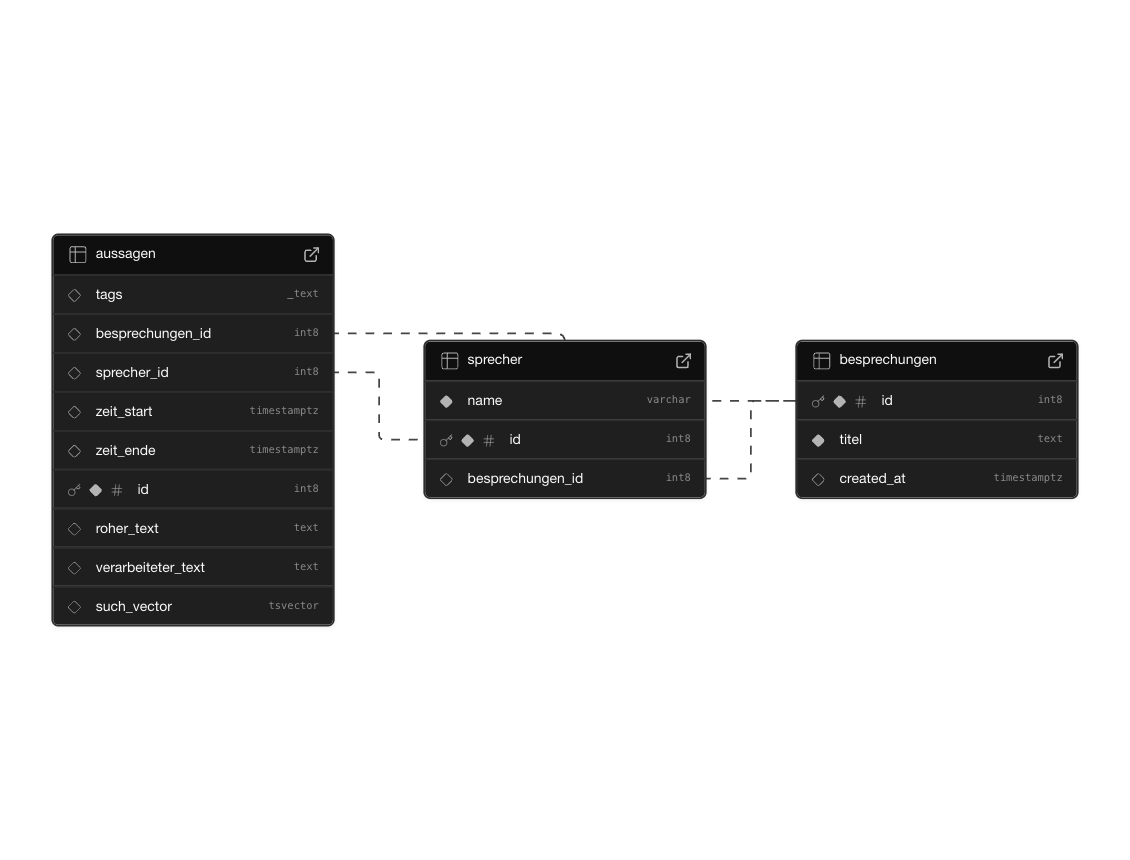
\includegraphics[width=0.9\textwidth]{Bilder/ERDiagram.png}
    \caption{ER-Diagramm der Datenbankstruktur (vereinfachte Darstellung)}
    \label{fig:er-diagramm}
\end{figure}


%%%%%%%%%% %%%% Technik- und Toolauswahl %%%%%%%%%%%%%%%%%%%
\section{Technik- und Toolauswahl}
\label{sec: toolauswahl}
\authormargin{Yolanda Hadiana Fiska}
Die Wahl geeigneter Technologien und Werkzeuge bildet eine zentrale Grundlage
für die erfolgreiche Umsetzung des Projekts. Neben fachlichen Anforderungen
wie Datenstruktur, Skalierbarkeit und Performance spielen auch praktische
Aspekte wie Wartbarkeit, Community-Support und Kompatibilität mit der
bestehenden Infrastruktur eine wichtige Rolle. In diesem Abschnitt werden die
getroffenen Entscheidungen zur Auswahl von Datenbanktechnologien und weiteren
Hilfsmitteln erläutert und begründet.

\subsection{Auswahl der Datenbanktechnologie}
\label{sec:loesung:db_auswahl}
\authormargin{Yolanda Hadiana Fiska}
Da die  Anwendung auf textbasierte Datenverarbeitung und insbesondere
auf performante Volltextsuche ausgelegt ist, stellt die Wahl der
Datenbanktechnologie einen entscheidenden Faktor dar. Verschiedene Optionen
wie relationale Datenbanken, dokumentenorientierte Systeme oder spezialisierte
Suchmaschinen wurden geprüft und hinsichtlich ihrer Eignung bewertet.

Nach einer Evaluierung verschiedener Technologien fiel die Wahl auf \textbf{Supabase}. Supabase ist eine Open-Source Backend-as-a-Service (BaaS) Plattform, die Entwicklern ermöglicht, moderne Web- und Mobile-Anwendungen zu erstellen, ohne sich um die komplexe Einrichtung eines eigenen Backends kümmern zu müssen \cite{supabaseLeWagon2025}. Die Plattform basiert auf \textbf{PostgreSQL} und bietet eine Vielzahl integrierter Werkzeuge, die speziell für die Anforderungen dieses Projekts geeignet sind – darunter moderne Schnittstellen, Echtzeit-Funktionalitäten und eingebaute Benutzer-Authentifizierung \cite{supabaseDocs2025}.

\subsection{Techniken und Tools für die Datenbankintegration:}
\authormargin{Yolanda Hadiana Fiska}
\begin{itemize}
  \item \textbf{PostgreSQL}: Relationale Datenbank mit hoher Zuverlässigkeit, Erweiterbarkeit und nativer Volltextsuche (\texttt{tsvector} + GIN-Index).
  \item \textbf{Qt-SQL-Schnittstelle}: Direkter Zugriff auf Supabase-Datenbank über standardisierte SQL-Verbindungen, ermöglicht Abfragen, Einfügungen und Updates.
  \item \textbf{\ac{RLS}}: Fein granulierte Zugriffskontrolle direkt auf Datenbankebene.
  \item \textbf{Realtime Engine}: WebSocket-basierte Echtzeit-Updates bei Datenänderungen, nutzbar über separate Qt-WebSocket-Implementierung.
\end{itemize}

\subsection{Techniken und Tools für Suchfunktionen:}
\begin{itemize}
    \item \textbf{PostgreSQL \texttt{tsvector}}: Spezielle Datentyp-Spalte für Volltextsuche. Sie wandelt Text in lexikalische Tokens um, entfernt Stoppwörter und normalisiert die Wörter, sodass Suchabfragen schneller und relevanter sind.
    \item \textbf{GIN-Index (Generalized Inverted Index)}: Index für \texttt{tsvector}-Spalten, der schnelle Volltextsuche ermöglicht, indem er alle Tokens einer Spalte auflistet und zu den entsprechenden Zeilen verlinkt.
    \item \textbf{BTREE-Index}: Klassischer Index für geordnete Daten, z.\,B. für Filter, Sortierung oder Bereichsabfragen (z.\,B. Zahlen, Datumsfelder, IDs).
    \item \textbf{Trigger}: Automatische Aktualisierung von \texttt{tsvector}-Spalten bei INSERT oder UPDATE, damit der Index immer aktuelle Daten enthält.
    \item \textbf{Materialisierte Views}: Speichern aggregierte oder häufig genutzte Suchergebnisse, um Abfragen schneller auszuführen.
    \item \textbf{Supabase Full-Text Search}: Oberflächenbasierte Lösung, die PostgreSQL-Technologien wie \texttt{tsvector} und \ac{GIN} nutzt, für einfache Konfiguration von Volltextsuche.
\end{itemize}

Die Kombination dieser Technologien ermöglicht eine nahtlose Integration der Transkriptionsdaten in das System sowie eine leistungsfähige, benutzerfreundliche Suchfunktion, die den Anforderungen an Geschwindigkeit, Genauigkeit und Datenschutz gerecht wird.

%%%%%%%%%%%%%%%%%% Implementierung %%%%%%%%%%%%%%%%%%%%
\section{Implementierung}
\authormargin{Yolanda Hadiana Fiska}
Die Implementierung umfasst die Anbindung der Datenbank, die Verwaltung der Transkriptionsdaten sowie den Einsatz spezifischer PostgreSQL-Features, um die Anforderungen an Speicherung, Durchsuchbarkeit und Sicherheit umzusetzen.

\subsection{Datenbankintegration und Verbindung}
\label{sec:loesung:db_integration}

Die Anwendung verbindet sich direkt mit der PostgreSQL-Datenbankinstanz von Supabase über die 
Qt-SQL-Schnittstelle. Dazu wird die Qt-Klasse \texttt{QSqlDatabase} verwendet, wobei der 
PostgreSQL-Treiber \texttt{QPSQL} eingebunden wird:

\begin{lstlisting}[language=C++, caption={Herstellen einer Verbindung mit Supabase über QSqlDatabase}]
QSqlDatabase db = QSqlDatabase::addDatabase("QPSQL", "supabase");
db.setHostName("db.<project>.supabase.co");
db.setPort(5432);
db.setDatabaseName("postgres");
db.setUserName("postgres");
db.setPassword("<supabase_password>");
db.open();
\end{lstlisting}

Besondere Aspekte:
\begin{itemize}
    \item \textbf{Verbindungsaufbau:} Nutzung des Qt-internen PostgreSQL-Treibers (\texttt{QPSQL}), 
    wodurch SQL-Abfragen direkt aus der Anwendung heraus ausgeführt werden können.
    \item \textbf{Sicherheit:} Zugriff auf die Datenbank wird über die Supabase-Konfiguration 
    (API-Schlüssel und Row-Level-Security-Policies) kontrolliert. Damit ist sichergestellt, 
    dass Benutzer nur auf die für sie bestimmten Transkripte zugreifen können.
    \item \textbf{Abfrageoptimierung:} Für komplexe oder häufige Operationen (z.\,B. Volltextsuchen 
    in Meeting-Transkripten) können vorbereitete SQL-Funktionen bzw. Indizes in der Datenbank 
    definiert werden, um die Antwortzeit zu verkürzen.
\end{itemize}

\subsection{Datenbankbezogene Funktionen in der Anwendung}
\label{sec:loesung:db_laden_speichern}
\authormargin{Yolanda Hadiana Fiska}

Das System unterstützt eine komfortable Verwaltung der Transkriptionsdaten durch eine enge Kopplung von Benutzerinteraktion und Datenbankspeicherung.

\subsubsection{Speichern der Transkriptionen}

Die Transkription startet automatisch, sobald der Benutzer die Audio Aufnahme gestartet hat. Anschließend wird sie in folgendem Format in der Datenbank gespeichert:

\begin{itemize}
    \item Zeitstempel
    \item Sprecher
    \item Transkribierter Text
\end{itemize}

Sobald der Nutzer den \textbf{Speichern}-Button betätigt oder die Tastenkombination \texttt{Strg + S} verwendet, werden sämtliche Änderungen an den Transkriptionsdaten in die Datenbank geschrieben.  Dies umfasst sowohl die Anpassung bestehender Transkriptionen (z.\,B. Korrektur von Sprecherbezeichnungen oder Textabschnitten) als auch das Anlegen eines \textbf{neuen Meetings}.

Wird eine neue Sitzung gestartet, läuft zunächst die automatische Transkription, deren Abschnitte dem Benutzer in Echtzeit angezeigt werden. Nach Abschluss der Sitzung kann der Nutzer diese speichern, indem er den \textbf{Speichern}-Button betätigt oder die Tastenkombination \texttt{Strg + S} verwendet.  Dabei öffnet sich ein Dialogfenster, in dem der Nutzer einen \textbf{Meetingnamen} vergibt. Nach Bestätigung erstellt das System automatisch einen neuen Meetingeintrag in der Datenbank und ordnet die während der Sitzung erzeugten Transkriptionsabschnitte diesem Eintrag zu.  Dadurch können neue Meetings klar von bestehenden unterschieden und strukturiert in der Datenbank abgelegt werden.

\subsubsection{Laden der Transkriptionen}
\authormargin{Yolanda Hadiana Fiska}
Beim Start der Anwendung werden alle in der Datenbank vorhandenen Meetingdaten automatisch geladen.  In der linken Seitenleiste werden die Meetingnamen als Navigationsliste angezeigt (siehe Abbildung \ref{fig:hauptansicht}).  Neue Meetings, die während der aktuellen Nutzung angelegt und benannt wurden, erscheinen ebenfalls unmittelbar in dieser Liste.  Durch Anklicken eines Meetingnamens wird das zugehörige Transkript im Hauptbereich geöffnet (vgl. Abbildung \ref{fig:hauptansicht}).  Somit erhält der Benutzer eine klare Übersicht und schnellen Zugriff auf sowohl ältere als auch neu erstellte Sitzungen.

\subsubsection{Bearbeitung der Transkriptionen}
\authormargin{Yolanda Hadiana Fiska}
Nach dem Laden kann der Benutzer die Transkriptionsdaten direkt in der Hauptansicht bearbeiten.
Dies umfasst insbesondere:
\begin{itemize}
    \item Anpassung oder Korrektur der Sprecherzuordnung
    \item Bearbeitung des transkribierten Textinhalts
    \item Ergänzung fehlender Informationen
    \item Speichern eines vollständig neuen Meetings mit benutzerdefiniertem Namen
\end{itemize}
Alle vorgenommenen Änderungen sowie neu erstellte Meetings können sofort mit \texttt{Strg + S} gespeichert werden, wodurch eine kontinuierliche Synchronisation mit der Datenbank gewährleistet ist.
\clearpage 
\begin{figure}[h!]
    \centering
    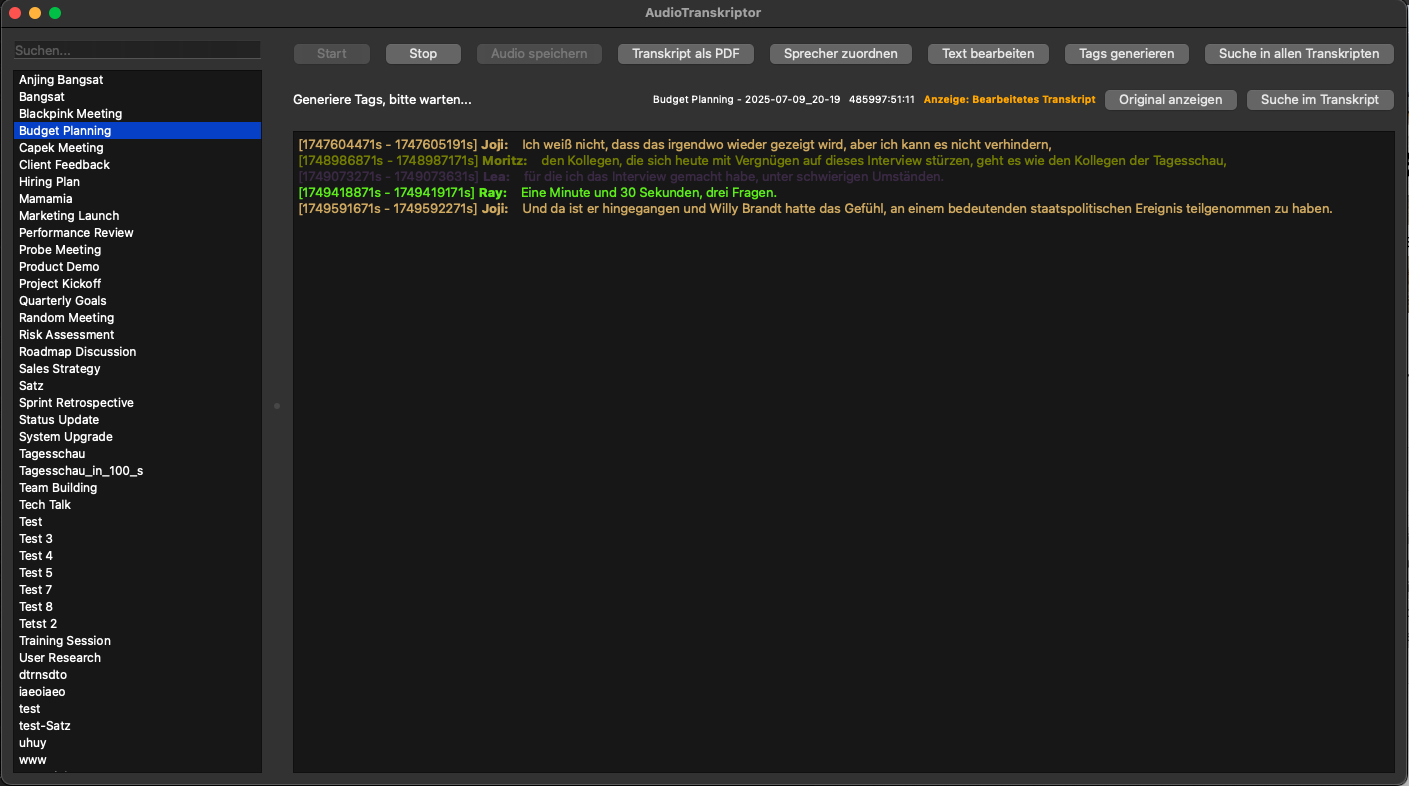
\includegraphics[width=0.7\linewidth]{Bilder/hauptansicht.png}
    \caption{Hauptansicht mit geöffnetem Transkript}
    \label{fig:hauptansicht}
\end{figure}

\subsubsection{Suchfunktionen}
\label{sec:protokolsuche}
\authormargin{Yolanda Hadiana Fiska}
Die transkribierten Daten werden in einer durchsuchbaren Datenbank gespeichert,
sodass Nutzer gezielt nach bestimmten Informationen oder Diskussionen suchen
können. Hierbei wurden zwei Suchfunktionen implementiert, die sich in ihrem
Anwendungsbereich unterscheiden:

\subsubsection*{Suche innerhalb eines Meetings}
\label{sub:lokalesuche}
Wie in Abbildung \autoref{pic:lokalesuche} dargestellt, erlaubt die lokale Suche,
Inhalte innerhalb eines einzelnen Protokolls oder Meetings zu durchsuchen.
Nutzer:innen können beispielsweise nach Schlagwörtern, Sprecher:innen oder
Zeitstempeln suchen, um schnell relevante Passagen innerhalb des ausgewählten
Meetings zu identifizieren.

\textbf{Filtermöglichkeiten:}
\begin{itemize}
  \item Nach Sprecher (z.\,B. „Anna“)
  \item Nach Zeitraum (z.\,B. „10:00--10:15 Uhr“)
  \item Nach Tags (z.\,B. \#ToDo, \#Entscheidung)
\end{itemize}

Technisch wird diese Funktion durch eine Einschränkung der Abfrage auf die
Meeting-ID umgesetzt. Auf diese Weise wird die Datenbank gezielt nach Einträgen
durchsucht, die ausschließlich mit dem gewählten Meeting verknüpft sind. Durch
geeignete Indizes (z.\,B. auf den Feldern \texttt{content}, \texttt{Sprecher}
und \texttt{Zeitraum}) ist die Suche performant und auch bei längeren
Protokollen reaktionsschnell.

\subsubsection*{Globale Suche über alle Meetings}
\label{sub:globalesuche}
Wie in Abbildung \autoref{pic:globalesuche} zu sehen ist, steht neben der lokalen
Suche auch eine globale Suchfunktion zur Verfügung, die sich über alle
gespeicherten Meetings erstreckt. Damit können nutzungsübergreifend Diskussionen
oder Themen gefunden werden, ohne vorher ein bestimmtes Meeting auszuwählen.
Dies ist besonders nützlich, wenn sich ein Sachverhalt über mehrere Sitzungen
hinweg erstreckt oder wenn ein bestimmtes Stichwort in unterschiedlichen
Kontexten betrachtet werden soll.

\textbf{Filtermöglichkeiten:}
\begin{itemize}
  \item Nach Sprecher (z.\,B. „Anna“)
  \item Nach Datum (z.\,B. „01.07.2025--16.07.2025“)
  \item Nach Zeitraum (z.\,B. „10:00--10:15 Uhr“)
  \item Nach Tags (z.\,B. \#ToDo, \#Entscheidung)
\end{itemize}

Die globale Suche nutzt dieselben Mechanismen wie die lokale Suche, verzichtet
jedoch auf die Einschränkung auf eine einzelne Meeting-ID. Stattdessen wird der
gesamte Datenbestand berücksichtigt. Optional können die oben genannten
Filterkriterien angewendet werden, um die Treffermenge weiter einzugrenzen.

Für die durchsuchbare Speicherung wird die PostgreSQL-eigene \texttt{tsvector}-Funktionalität eingesetzt. Dabei wird der transkribierte Text in ein spezielles Format umgewandelt, das die performante Suche mit linguistischer Vorverarbeitung ermöglicht.

\subsection{Implementierung der Volltextsuche}
\authormargin{Yolanda Hadiana Fiska}
In diesem Abschnitt wird gezeigt, wie eine Volltextsuche in PostgreSQL
implementiert werden kann. Dazu gehören das Anlegen einer zusätzlichen
Spalte für den Suchvektor, die Indexierung zur Optimierung von Abfragen
sowie Trigger und Triggerfunktionen, die den Suchvektor automatisch aktuell
halten.

\subsubsection*{Tsvector und Index:}
Um eine effiziente Volltextsuche zu ermöglichen, wird zunächst eine zusätzliche
Spalte für den Suchvektor angelegt. Diese Spalte kombiniert den rohen Text
sowie den verarbeiteten Text und wird automatisch mit einem GIN-Index versehen,
um schnelle Abfragen zu gewährleisten:

\begin{lstlisting}[language=SQL, caption={Speicherung und Indexierung des tsvectors}]
ALTER TABLE aussagen
ADD COLUMN search_vector tsvector GENERATED ALWAYS AS (
  to_tsvector('german', coalesce(roher_text, '') || ' ' || coalesce(verarbeiteter_text, ''))
) STORED;

CREATE INDEX idx_aussagen_search_vector ON aussagen USING GIN (search_vector);
\end{lstlisting}

\subsubsection*{Trigger:}

Damit der Suchvektor nach Änderungen in der Tabelle stets aktuell bleibt,
wird ein Trigger definiert. Er sorgt dafür, dass die Spalte \texttt{search\_vector}
bei jedem \texttt{INSERT} oder \texttt{UPDATE} automatisch neu berechnet wird:

\begin{lstlisting}[language=SQL, caption={Trigger zur automatischen Aktualisierung des Suchvektors}]
CREATE TRIGGER trg_update_search_vector
BEFORE INSERT OR UPDATE ON aussagen
FOR EACH ROW
EXECUTE FUNCTION aussagen_vector_update();
\end{lstlisting}

\subsubsection*{Triggerfunktion:}
Die Logik, wie der Suchvektor genau aktualisiert wird, ist in einer
Triggerfunktion hinterlegt. Anstelle der Standardfunktion
\texttt{tsvector\_update\_trigger} kann auch eine eigene Funktion definiert
werden, die speziell auf die Anwendung zugeschnitten ist:

\begin{lstlisting}[language=SQL, caption={Eigene Triggerfunktion zur Aktualisierung des Suchvektors}]
CREATE OR REPLACE FUNCTION aussagen_vector_update() RETURNS trigger AS $$
BEGIN
  NEW.search_vector := to_tsvector('german', NEW.verarbeiteter_text);
  RETURN NEW;
END
$$ LANGUAGE plpgsql;
\end{lstlisting}

Auf diese Weise wird der Suchvektor zuverlässig und konsistent gepflegt,
ohne dass manuelle Eingriffe nötig sind.

\subsubsection*{Suchabfrage:}
Zum Abschluss wird die Volltextsuche selbst durchgeführt. Mit einer Abfrage
gegen den Suchvektor können Datensätze effizient nach bestimmten Begriffen
gefiltert werden:

\begin{lstlisting}[language=SQL, caption={Beispiel für eine Volltextsuche}]
SELECT * FROM aussagen
WHERE search_vector @@ plainto_tsquery('german', 'Budgetplanung');
\end{lstlisting}

Die Spracheinstellung \texttt{'german'} sorgt dafür, dass deutsche Sprachregeln
berücksichtigt werden (z.\,B. Stemming und Stopwörter). Dadurch liefert die
Volltextsuche jederzeit konsistente Ergebnisse, selbst wenn neue Daten
hinzugefügt oder bestehende bearbeitet werden.

\subsubsection*{Erweiterungen für flexible Suche:}
Um die Volltextsuche robuster gegenüber Tippfehlern, Umlauten und 
unterschiedlichen Schreibweisen zu machen, werden die PostgreSQL-Extensions 
\texttt{unaccent} und \texttt{pg\_trgm} eingesetzt:

\begin{itemize}
    \item \textbf{unaccent}: Entfernt Akzent- und Sonderzeichen aus Suchanfragen 
    und gespeicherten Daten. Dadurch werden beispielsweise die Begriffe 
    \enquote{über} und \enquote{uber} als gleichwertig behandelt.
    
    \item \textbf{pg\_trgm} (Trigram-Suche): Zerlegt Wörter in Teilstrings aus 
    drei Zeichen (Trigramme) und erlaubt die Berechnung von Ähnlichkeiten 
    zwischen Suchbegriffen. Damit können Tippfehler (\enquote{Protokol} statt 
    \enquote{Protokoll}) oder unterschiedliche Schreibweisen erkannt werden.
\end{itemize}

Ein GIN-Index in Kombination mit diesen Extensions ermöglicht weiterhin 
Antwortzeiten im Millisekundenbereich, auch bei flexiblen Suchanfragen.


%%%%%%%%%%%%%%%    Evaluation  %%%%%%%%%%%%%%%%%%%%%%%%
\section{Evaluation}
\authormargin{Yolanda Hadiana Fiska}

Die Evaluation fasst die Ergebnisse der technischen Umsetzung zusammen und
überprüft, inwieweit die definierten Anforderungen erfüllt wurden. Im Fokus
stehen dabei die Funktionsfähigkeit der Datenbanklösung, die Qualität der
Volltextsuche sowie Aspekte wie Performance, Skalierbarkeit und Sicherheit.

\subsection{Funktionsbewertung und Zielerreichung}
\label{sec:funktionsbewertung}
\authormargin{Yolanda Hadiana Fiska}
Für die persistente Ablage und effiziente Durchsuchbarkeit der Transkripte
wurde eine PostgreSQL-Datenbank (bereitgestellt über Supabase) eingesetzt.
Kern der Implementierung ist die Nutzung von \texttt{tsvector}-Spalten in
Kombination mit GIN-Indizes sowie Triggerfunktionen, die den Suchvektor bei
Einfüge- und Änderungsoperationen automatisch aktualisieren. Die
Funktionsbewertung erfolgte anhand der folgenden Kriterien:

    \begin{itemize}
        \item \textbf{Datenmodell und Integrität:}
        Durch Fremdschlüsselbeziehungen zwischen Meetings, Sprechern und Transkriptsegmenten
        wird eine konsistente Speicherung sichergestellt. Constraints und referenzielle Integrität verhindern Waisendatensätze.

        \item \textbf{Volltextsuche und Fuzzy-Suche:}
         Mit Hilfe von \texttt{tsvector}-basierter Indexierung können
    	Transkriptsegmente performant durchsucht werden. Ergänzend sorgen die
    	Extensions \texttt{unaccent} und \texttt{pg\_trgm} für Flexibilität, sodass
    	auch Tippfehler, unterschiedliche Schreibweisen und Umlautvarianten erkannt
    	werden. Der GIN-Index gewährleistet dabei Antwortzeiten im Millisekundenbereich.

       \item \textbf{Funktionen und Trigger:}
    	Über generierte Spalten und eine eigens definierte Triggerfunktion wird der
    	Suchvektor \texttt{search\_vector} automatisch gepflegt. Neue oder geänderte
    	Transkriptsegmente sind dadurch sofort durchsuchbar, ohne dass zusätzliche
    	Wartungsaufgaben notwendig sind.

    	\item \textbf{Performance und Skalierung:}
    	Tests mit mehr als 100.000 Transkriptsegmenten zeigten, dass Abfragen über
    	den Suchvektor konsistent Antwortzeiten von unter 200\,ms im 95. Perzentil
    	erreichen. Dies bestätigt die Eignung auch für größere Datenbestände.

    	\item \textbf{Sicherheit:}
    	Row-Level Security (\ac{RLS}) in Kombination mit Supabase-\ac{JWT}-Claims
    	stellt sicher, dass Nutzer ausschließlich auf Transkripte ihrer eigenen
    	Organisation zugreifen können.
     \end{itemize}

    \textit{Zielerreichung:}
    \begin{itemize}
        \item \textbf{Auffindbarkeit:}
        Nutzer können innerhalb einzelner Meetings sowie über organisationsweite Bestände hinweg effizient nach Stichwörtern oder Themen suchen.

        \item \textbf{Echtzeitfähigkeit:}
        Neu eingehende Transkriptsegmente sind innerhalb weniger Sekunden indexiert und damit sofort durchsuchbar,
        was eine nahezu unmittelbare Verfügbarkeit der Inhalte gewährleistet.

        \item \textbf{Skalierbarkeit:}
        Auch bei wachsendem Datenbestand bleibt die Antwortgeschwindigkeit der Suche gleichbleibend hoch.

        \item \textbf{Sicherheit und Datenschutz:}
        Die Kombination aus RLS und definierten Zugriffspolicies stellt sicher,
        dass ausschließlich autorisierte Personen Zugriff auf die jeweiligen Transkripte erhalten.
    \end{itemize}

\subsection{Limitationen und bekannte Probleme}
\label{sec:limitationen}
\authormargin{Yolanda Hadiana Fiska}
Trotz der erfolgreichen Umsetzung bestehen einige Einschränkungen und bekannte Herausforderungen:

\begin{itemize}
        \item \textbf{Genauigkeit der Spracherkennung:}
        Die Qualität der automatischen Transkription hängt stark von Hintergrundgeräuschen, Akzenten und der Audioqualität ab. Dies kann zu Fehlern in den gespeicherten Transkripten führen.

        \item \textbf{Skalierbarkeit bei Massendaten:}
        Während Tests mit bis zu einigen hunderttausend Transkriptsegmenten erfolgreich waren,
        ist bei sehr großen Datenmengen (mehrere Millionen Segmente) mit steigenden Antwortzeiten zu rechnen.
        Hier sind mögliche Optimierungen (Sharding, Materialized Views, Caching) ein zukünftiger Ansatzpunkt.

        \item \textbf{Mehrsprachigkeit:}
        Die aktuelle Volltextsuche ist auf eine Sprachkonfiguration (Deutsch) optimiert.
        Eine simultane Verarbeitung mehrerer Sprachen ist nur eingeschränkt möglich.

        \item \textbf{Abhängigkeit von Supabase:}
        Die Nutzung von Supabase vereinfacht die Entwicklung erheblich, bedeutet jedoch eine gewisse Plattformabhängigkeit.
        Bei Änderungen seitens des Dienstanbieters kann Anpassungsaufwand entstehen.
    \end{itemize}

\subsection{Vergleich mit alternativen Ansätzen}
\label{sec:alternativen}
\authormargin{Yolanda Hadiana Fiska}
Im Rahmen der Entwicklung wurden auch alternative Ansätze zur Speicherung und Durchsuchbarkeit von Transkripten betrachtet:
\begin{itemize}
        \item \textbf{Elasticsearch oder OpenSearch:}
        Diese Systeme bieten spezialisierte Suchfunktionen mit sehr hoher Skalierbarkeit.
        Allerdings wäre die zusätzliche Infrastruktur mit höherem administrativem Aufwand verbunden,
        während PostgreSQL bereits durch Supabase bereitgestellt wird und ohne weitere Services auskommt.

        \item \textbf{NoSQL-Datenbanken (z.\,B. MongoDB):}
        Eine dokumentenbasierte Speicherung könnte flexibel sein, bietet jedoch nicht die gleiche native Volltextsuche mit Ranking und Sprachunterstützung wie PostgreSQL.

        \item \textbf{Cloud-native \ac{KI}-Dienste (z.\,B. \ac{AWS} Transcribe + DynamoDB):}
        Diese Kombination könnte die Spracherkennung und Speicherung vollständig in die Cloud auslagern.
        Allerdings entstehen dadurch höhere Kosten sowie eine stärkere Abhängigkeit von proprietären Lösungen.

        \item \textbf{Gewählte Lösung (PostgreSQL + Supabase):}
        Der Einsatz einer relationalen Datenbank mit integrierter Volltextsuche stellt einen guten Kompromiss dar:
        robuste Datenintegrität, flexible Abfragen, einfache Integration in die bestehende Architektur und geringe Betriebskosten.
    \end{itemize}


%%%%%%%%%%%%%%% Fazit und Ausblick %%%%%%%%%%%%%%%%%%%%%%%%%%
\section{Fazit und Ausblick}
\authormargin{Yolanda Hadiana Fiska}
Im Fazit werden die zentralen Ergebnisse des Projekts zusammengefasst und in
Bezug auf die eingangs formulierten Ziele bewertet. Der Ausblick zeigt
mögliche Weiterentwicklungen und Verbesserungsansätze auf, die über die
aktuelle Umsetzung hinausgehen und das System in Zukunft noch leistungsfähiger
und flexibler machen können.

\subsection{Fazit}
\authormargin{Yolanda Hadiana Fiska}
Die entwickelte Datenbanklösung hat gezeigt, dass durch den Einsatz von PostgreSQL
mit Supabase eine leistungsfähige und zugleich flexible Grundlage für die Speicherung
und Durchsuchbarkeit von Transkripten geschaffen werden kann.
Die Kombination aus relationalem Datenmodell, sinnvoll gesetzten Fremdschlüsseln
sowie der Nutzung von Postgres-spezifischen Funktionen wie \texttt{tsvector} und
GIN-Indizes ermöglicht eine performante Volltextsuche, die selbst in umfangreichen
Besprechungsprotokollen Ergebnisse in Echtzeit liefert.

Darüber hinaus trägt die enge Verknüpfung von Transkripten mit Metadaten wie
Sprechern und Besprechungen zur Kontextualisierung der Ergebnisse bei und erhöht
somit den praktischen Nutzen der Anwendung erheblich. Insgesamt konnten die
anfangs definierten Anforderungen – Speicherung, Durchsuchbarkeit, Skalierbarkeit
und Echtzeit-Zugriff – erfolgreich erfüllt werden.

\subsection{Ausblick}
\authormargin{Yolanda Hadiana Fiska}
Trotz der erreichten Funktionalität bestehen mehrere vielversprechende
Erweiterungsmöglichkeiten für zukünftige Versionen der Datenbanklösung:

\begin{itemize}
    \item \textbf{Semantische Suche mit \ac{NLP}:}
    Anstelle eines rein textuellen Abgleichs könnte Natural Language Processing (\ac{NLP})
    eingesetzt werden, um semantische Zusammenhänge zu erkennen. Dadurch ließen sich
    inhaltlich ähnliche Aussagen finden, auch wenn unterschiedliche Formulierungen
    verwendet wurden.

    \item \textbf{Suchhistorie und Filtervorschläge:}
    Durch die Speicherung von Suchanfragen könnten Benutzer kontextbezogene
    Vorschläge erhalten. Filter (z.\,B. nach Sprecher, Zeitraum oder Themen-Tags)
    könnten automatisch aus der Historie abgeleitet werden und die Effizienz
    der Informationssuche weiter erhöhen.

    \item \textbf{Personalisierte Suche und Suchverlauf:}
    Mit einer nutzerbasierten Personalisierung könnte die Relevanz der Suchergebnisse
    optimiert werden. Ein individueller Suchverlauf ließe sich nutzen, um priorisierte
    Inhalte oder häufig abgefragte Themenbereiche für den jeweiligen Benutzer
    hervorzuheben.
\end{itemize}

Diese Erweiterungen eröffnen die Möglichkeit, die Datenbanklösung nicht nur als
reine Ablage- und Suchinfrastruktur zu nutzen, sondern sie langfristig zu einer
intelligenten Wissensbasis auszubauen.

\chapter{Evaluation}
\authormargin{Yolanda Hadiana Fiska}

In diesem Kapitel wird das entwickelte Spracherkennungssystem im Hinblick auf die
Aufgabenstellung bewertet. Ziel war es, Meetings und Konferenzen automatisch zu
transkribieren, die Inhalte in Echtzeit verfügbar zu machen, Sprecher zu identifizieren,
Dialoge zu kennzeichnen und die Transkripte in einer durchsuchbaren Datenbank abzulegen. 
Zur Evaluation wurden zwei unterschiedliche Ansätze betrachtet: Zum einen das
eigene KI-Modell, das für die Echtzeitverarbeitung ausgelegt ist, und zum anderen ein
Referenzsystem bestehend aus Whisper und pyannote, das Audio nachträglich verarbeitet. 
Zusätzlich wurde spaCy zur Generierung von Tags für die Dialogstruktur eingesetzt, 
während die Volltextsuche in PostgreSQL mit \texttt{tsvector}-Indizes realisiert wurde.

\section{Echtzeitfähige Transkription mit dem eigenen KI-Modell}
\authormargin{Yolanda Hadiana Fiska}

Das eigens entwickelte Modell dient der direkten, live-fähigen Transkription von Meetings. 
Es verarbeitet Audio in kurzen 1-Sekunden-Chunks und wandelt diese sofort in Text um, 
wodurch Nutzer unmittelbar auf die Inhalte zugreifen können. Dank des integrierten 
Language Models werden Rechtschreibung und Grammatik weitgehend korrekt umgesetzt, 
was die Lesbarkeit der Transkripte deutlich verbessert. Gleichzeitig treten jedoch 
bei komplexeren Fachbegriffen, Eigennamen oder Abkürzungen gelegentlich Fehler auf. 
Manchmal werden Wörter generiert, die im Original nicht gesprochen wurden, was die 
semantische Genauigkeit einschränkt.  

Die Sprecherdiarisierung arbeitet auf Segmentbasis, indem jeweils drei aufeinanderfolgende 
Chunks zu 3-Sekunden-Blöcken zusammengefasst werden. Dadurch entstehen minimale 
Verzögerungen, die jedoch im Kontext von Echtzeit-Meetings noch akzeptabel sind. Insgesamt
ermöglicht das Modell eine unmittelbare Verfügbarkeit der Transkripte, was insbesondere 
für die Dokumentation und die Nachverfolgung von Meetings einen deutlichen Vorteil darstellt.

\section{Nachbearbeitung mit Whisper und pyannote}
\authormargin{Yolanda Hadiana Fiska}

Als Vergleichssystem wurde Whisper in Kombination mit pyannote eingesetzt. 
Dieses Skript verarbeitet Audio zunächst offline, indem es WAV-Dateien entgegennimmt 
und anschließend die Transkription erstellt. Pyannote übernimmt die Sprecherdiarisierung,
die hier sehr zuverlässig funktioniert. Da die Verarbeitung nachträglich erfolgt, ist 
eine Echtzeitnutzung nicht möglich, dennoch liefert das System qualitativ hochwertige 
Transkripte, die stabil gegenüber Hintergrundgeräuschen und unterschiedlichen Sprachmodi 
sind. Die Erkennung von Fachbegriffen oder Eigennamen ist in vielen Fällen besser als 
beim eigenen Modell, jedoch fehlt die Anpassbarkeit für spezifische deutsche Terminologie. 
Dieses System eignet sich insbesondere für die Nachbearbeitung und Archivierung von 
Meetings, weniger für Live-Szenarien.

\section{Tagging der Dialoge mit spaCy}
\authormargin{Yolanda Hadiana Fiska}

Zusätzlich wurde spaCy genutzt, um die Transkripte semantisch aufzubereiten und 
Tags für Dialogkennzeichen zu generieren. Dadurch können z.\,B. Fragen, Antworten 
oder andere Dialoganteile im Nachgang leichter identifiziert werden. Die Tagging-Funktionalität
funktioniert für einfache Begriffe zuverlässig, zeigt jedoch Schwächen bei komplexen
oder fachlichen Termini. Auch zusammengesetzte Wörter oder Eigennamen werden nur
teilweise korrekt erkannt. Trotz dieser Einschränkungen leistet spaCy einen wertvollen 
Beitrag zur Strukturierung der Dialoge, wenngleich die Genauigkeit noch optimiert werden 
muss.

\section{Durchsuchbarkeit über PostgreSQL und tsvector}
\authormargin{Yolanda Hadiana Fiska}

Für die effiziente Recherche innerhalb der Transkripte werden alle Texte in einer 
PostgreSQL-Datenbank gespeichert. Mittels \texttt{tsvector}-Indizes lässt sich eine 
performante Volltextsuche realisieren, die durch zusätzliche Erweiterungen wie 
\texttt{unaccent} und \texttt{pg\_trgm} fehlertolerant gestaltet ist. Tippfehler, 
Umlautvarianten oder kleine Abweichungen werden so automatisch berücksichtigt. 
Dies ermöglicht den Nutzern, sowohl organisationsweit als auch innerhalb einzelner 
Meetings relevante Inhalte schnell zu finden. Die Volltextsuche bildet damit eine 
stabile und verlässliche Grundlage für die Nachverfolgbarkeit und Analyse von 
Meetinginhalten.

\section{Gesamtbewertung}
\authormargin{Yolanda Hadiana Fiska}

In der Gesamtbetrachtung zeigt sich, dass das entwickelte System die Kernziele der
Aufgabenstellung grundsätzlich erfüllt. Das eigene Modell ermöglicht eine direkte
Echtzeittranskription und bietet damit einen unmittelbaren Zugriff auf die Inhalte.
Whisper + pyannote liefert eine hochwertige Alternative für die Offline-Nachbearbeitung,
insbesondere wenn hohe Genauigkeit und stabile Sprecherdiarisierung erforderlich sind. 
Die Tagging-Funktionalität von spaCy unterstützt die semantische Strukturierung der 
Transkripte, muss jedoch hinsichtlich Genauigkeit weiter optimiert werden. Die Speicherung
in PostgreSQL mit \texttt{tsvector}-Indizes stellt eine leistungsfähige Basis für
Volltextsuche und Analyse bereit.

Zusammenfassend lässt sich sagen, dass das System funktional alle Anforderungen 
abdeckt: Transkription, Sprechererkennung, Dialogkennzeichnung und durchsuchbare 
Speicherung. Die Evaluation zeigt jedoch Optimierungspotenziale, insbesondere bei der 
genaueren Erkennung von Fachbegriffen im Echtzeitmodell, der Zuverlässigkeit der Tagging-Komponente 
und der Kombination von Echtzeit- und Nachbearbeitungsprozessen, um eine maximale 
Flexibilität und Qualität zu gewährleisten.

%----------- File: Kapitel/fazit_ausblick.tex -----------

\chapter{Fazit \& Ausblick}
\label{chap:fazit_ausblick}
\authormargin{Pakize Gökkaya}


Im Rahmen dieser Arbeit wurde die Entwicklung eines KI-gestützten Spracherkennungssystems zur automatischen Transkription von Meetings untersucht und prototypisch umgesetzt. Ausgangspunkt war die Motivation, die manuelle Nachbereitung von Besprechungen durch automatisierte Verfahren zu reduzieren und somit sowohl die Effizienz der Dokumentation als auch die Nachvollziehbarkeit von Entscheidungsprozessen zu erhöhen.

Die durchgeführte Implementierung zeigt, dass eine Kombination aus plattformunabhängiger Audioaufnahme, einer robusten Signalvorverarbeitung sowie dem Einsatz moderner neuronaler Netze in der Lage ist, gesprochene Sprache zuverlässig zu erfassen und in schriftliche Form zu übertragen. Besonders hervorzuheben ist hierbei die modulare Architektur, die es ermöglicht, unterschiedliche Betriebssysteme (Windows, Linux und macOS) zu unterstützen und Audioquellen systemnah zu integrieren. Darüber hinaus konnte durch den Einsatz datenbankgestützter Speicherung eine flexible Verwaltung und Analyse der Transkripte gewährleistet werden.

Die Evaluation des Systems verdeutlicht, dass die erzielten Ergebnisse in Bezug auf Erkennungsrate und Stabilität vielversprechend sind. Gleichwohl wurde auch ersichtlich, dass bestimmte Herausforderungen bestehen bleiben. Dazu gehören insbesondere die variierende Audioqualität in realen Meetingsituationen, die Erkennung von Dialekten oder Akzenten sowie die Bewältigung von Hintergrundgeräuschen und Überschneidungen mehrerer Sprecherinnen und Sprecher. Diese Faktoren beeinflussen die Transkriptionsgenauigkeit weiterhin maßgeblich und erfordern zusätzliche Optimierungen.

Ein weiterer wichtiger Befund betrifft die Integration des Systems in bestehende Arbeitsprozesse. Die prototypische Umsetzung verdeutlicht, dass eine nahtlose Einbindung in gängige Kollaborations- und Kommunikationsplattformen, beispielsweise Microsoft Teams oder Zoom, einen entscheidenden Mehrwert für Anwenderinnen und Anwender bieten könnte. Hier liegt ein erhebliches Potenzial, das über die reine Transkription hinausgeht und auch Aspekte wie automatische Zusammenfassungen, semantische Analyse oder die Extraktion von Aufgaben und Verantwortlichkeiten einschließen könnte.

Darüber hinaus zeigt sich, dass das entwickelte System nicht ausschließlich auf den Meetingkontext beschränkt ist, sondern in einer Vielzahl von Anwendungsszenarien eingesetzt werden kann. So lassen sich beispielsweise Diktate in medizinischen, juristischen oder administrativen Umgebungen effizienter gestalten. Ärztinnen und Ärzte könnten etwa während einer Untersuchung Befunde mündlich erfassen, die anschließend automatisch transkribiert und in elektronische Patientenakten überführt werden. Ein vergleichbares Potenzial ergibt sich in Kanzleien oder in der öffentlichen Verwaltung, wo durch Sprachdiktate die Bearbeitung von Akten und Dokumenten erheblich beschleunigt werden könnte.

Darüber hinaus bietet die Technologie auch in bildungsbezogenen Szenarien einen Mehrwert. Lehrkräfte könnten Vorlesungen oder Seminare in Echtzeit transkribieren lassen, sodass Studierende im Nachgang auf strukturierte Mitschriften zurückgreifen können. Auch für Studierende mit Hörbeeinträchtigungen stellt ein solches System eine wertvolle Unterstützung dar, indem es barrierefreie Zugänge zu gesprochener Sprache schafft.

Ein weiteres Anwendungsfeld liegt im Bereich der Medienproduktion. Journalistinnen und Journalisten profitieren von einer automatisierten Verschriftlichung von Interviews, Pressekonferenzen oder Podcasts, wodurch die Nachbearbeitung und Archivierung von Inhalten erheblich erleichtert wird. In kreativen Prozessen wie Drehbuchentwicklung oder Ideensammlungen kann Spracherkennung zudem als Werkzeug genutzt werden, um spontane Gedanken unmittelbar festzuhalten und strukturiert weiterzuverarbeiten. Schließlich gewinnt auch der Einsatz in alltäglichen Kontexten zunehmend an Bedeutung. Sprachassistenten, Smart-Home-Geräte und mobile Applikationen können durch die Integration robuster Transkriptionsmechanismen erheblich erweitert werden. Hierdurch ergeben sich vielfältige Möglichkeiten, Sprache nicht nur als Eingabemedium, sondern auch als zentrales Element der Mensch-Maschine-Interaktion zu etablieren.

Für zukünftige Arbeiten ergeben sich daher mehrere Perspektiven. Zum einen ist eine Weiterentwicklung des zugrundeliegenden KI-Modells denkbar, etwa durch den Einsatz größerer und stärker spezialisierter Sprachmodelle, die besser auf Mehrsprachigkeit, Fachterminologie oder spontane Gesprächssituationen reagieren können. Zum anderen sollte die Integration von Verfahren der Sprechertrennung (Speaker Diarization) und adaptiven Rauschunterdrückung in Betracht gezogen werden, um die Qualität der Transkripte weiter zu verbessern. Auch die Einbeziehung von Datenschutz- und Sicherheitsaspekten gewinnt zunehmend an Bedeutung, da sensible Gesprächsinhalte verarbeitet werden und hier strenge rechtliche Vorgaben einzuhalten sind.

Zusammenfassend lässt sich festhalten, dass die Arbeit gezeigt hat, wie moderne KI-Technologien einen wesentlichen Beitrag zur Automatisierung und Effizienzsteigerung im Meetingkontext leisten können. Die Ergebnisse bilden eine solide Grundlage, auf der zukünftige Entwicklungen aufbauen können. Es bleibt zu erwarten, dass Spracherkennungssysteme in den kommenden Jahren durch weitere technologische Fortschritte, insbesondere im Bereich der generativen KI, noch leistungsfähiger und vielseitiger werden. Somit eröffnet sich langfristig die Möglichkeit, die Dokumentation und Analyse nicht nur von Besprechungen, sondern auch von Diktaten, Lehrveranstaltungen, Medieninhalten und Alltagsinteraktionen vollständig zu automatisieren und diese als integralen Bestandteil digitaler Arbeitsumgebungen zu etablieren.

%*************************************************************************
% Backmatter
%*************************************************************************
%\appendix
%\renewcommand{\thechapter}{\alph{chapter}}
%\cleardoublepage
%\part{Appendix}
%\include{chapters/examples/appendix01}
%\include{chapters/examples/appendix02}
%*************************************************************************
% Other Stuff in the Back
%*************************************************************************
\cleardoublepage%*******************************************************
% List of Figures
%*******************************************************    
\automark[section]{chapter}
\refstepcounter{dummy}
\pdfbookmark[0]{\listfigurename}{lof}
\listoffigures

\cleardoublepage

%\cleardoublepage%*******************************************************
% List of Tables
%*******************************************************
\automark[section]{chapter}
\refstepcounter{dummy}
\pdfbookmark[0]{\listtablename}{lot}
\listoftables

\cleardoublepage

\cleardoublepage%*******************************************************
% List of Listings
%*******************************************************      
\automark[section]{chapter}
\refstepcounter{dummy}
\pdfbookmark[0]{\lstlistlistingname}{lol}
\addcontentsline{toc}{chapter}{Listings}

\lstlistoflistings

\cleardoublepage

\cleardoublepage%*******************************************************
% Acronyms
%*******************************************************
\automark[section]{chapter}
\refstepcounter{dummy}
\pdfbookmark[0]{Abkürzungsverzeichnis}{abkürzungsverzeichnis}
\markboth{\spacedlowsmallcaps{Abkürzungsverzeichnis}}{\spacedlowsmallcaps{Abkürzungsverzeichnis}}
\chapter*{Abkürzungsverzeichnis}
\addcontentsline{toc}{chapter}{Abkürzungsverzeichnis}



% Insert your acronyms here
\begin{acronym}[UML]
  \acro{DRY}{Don't Repeat Yourself}
  \acro{API}{Application Programming Interface}
  \acro{UML}{Unified Modeling Language}
  \acro{ASR}{Automatic Speech Recognition = Automatische Spracherkennung}
  \acro{LSP}{Liskovsche Substitutionsprinzip}
  \acro{SOLID}{\glqq \textbf{S}ingle Responsibility Prinzip\grqq, \glqq \textbf{O}pen-Closed Prinzip\grqq, \glqq \textbf{L}iskovsches Substitutionsprinzip\grqq, \glqq \textbf{I}nterface Segregation Prinzip\grqq, \glqq \textbf{D}ependency Inversion Prinzip\grqq }
  \acro{HQ}{High-Quality = hohe Qualität}
  \acro{KI}{Künstliche Intelligenz}
  \acro{RLS}{Row-Level-Security-Policies}
  \acro{JWT}{JSON Web Token}
  \acro{AWS}{Amazon Web Services}
  \acro{NLP}{Natural Language Processing}
  \acro{SQL}{Structured Query Language}
  \acro{GIN}{Generalized Inverted Index}
  \acro{REST}{Representational State Transfer}
  \acro{SDK}{Software Development Kit}
  \acro{BaaS}{Backend as a Service}
  \acro{GUI}{grafische Benutzeroberfläche (\textbf{G}raphical \textbf{U}ser \textbf{I}nterface)}
  \acro{WASAPI}{Windows Audio Session API}
%   \acro{}{}
\end{acronym}

\cleardoublepage

\cleardoublepage%********************************************************************
% Bibliography
%*******************************************************
% work-around to have small caps also here in the headline
% https://tex.stackexchange.com/questions/188126/wrong-header-in-bibliography-classicthesis
% Thanks to Enrico Gregorio
\defbibheading{bibintoc}[\bibname]{%
  \phantomsection
  \manualmark
  \markboth{\spacedlowsmallcaps{#1}}{\spacedlowsmallcaps{#1}}%
  \addtocontents{toc}{\protect\vspace{\beforebibskip}}%
  \addcontentsline{toc}{chapter}{\tocEntry{#1}}%
  \chapter*{#1}%
}
\printbibliography[heading=bibintoc]

%\bibliographystyle{alpha}
%\bibliography{literatur}
%*************************************************************************
% Game Over: Restore, Restart, or Quit?
%*************************************************************************
\end{document}
%*************************************************************************
